\section{Gerät Aufbau}

\subsection{CAD-Baugruppe}

Das Gerät wurde im CAD modelliert. In der CAD-Baugruppe wurden neben den eigens vom Team konstruierten Teilen auch die Normteilen für die Hub- und die Fortbewegungsmotoren dargestellt. Elektronik Komponenten wie beispielsweise der Controller, Kamera oder Sensoren wurden mithilfe von Vorlagen\footnote{\url{https://grabcad.com/}} in die Zeichnung integriert. In der Abbildung \ref{fig:CADohneHaube1} ist die CAD-Baugruppe seitlich von vorne zusehen und in der Abbildung \ref{fig:CADohneHaube2} seitlich von hinten. Bei beiden Bildern ist das Gerät ohne Haube dargestellt, um den inneren Aufbau ersichtlich zu machen. Eine Abbildung des CAD-Modells der Haube ist im Kapitel \ref{subsec:Komponenten} am Ende zu finden.

\begin{figure}[H]
  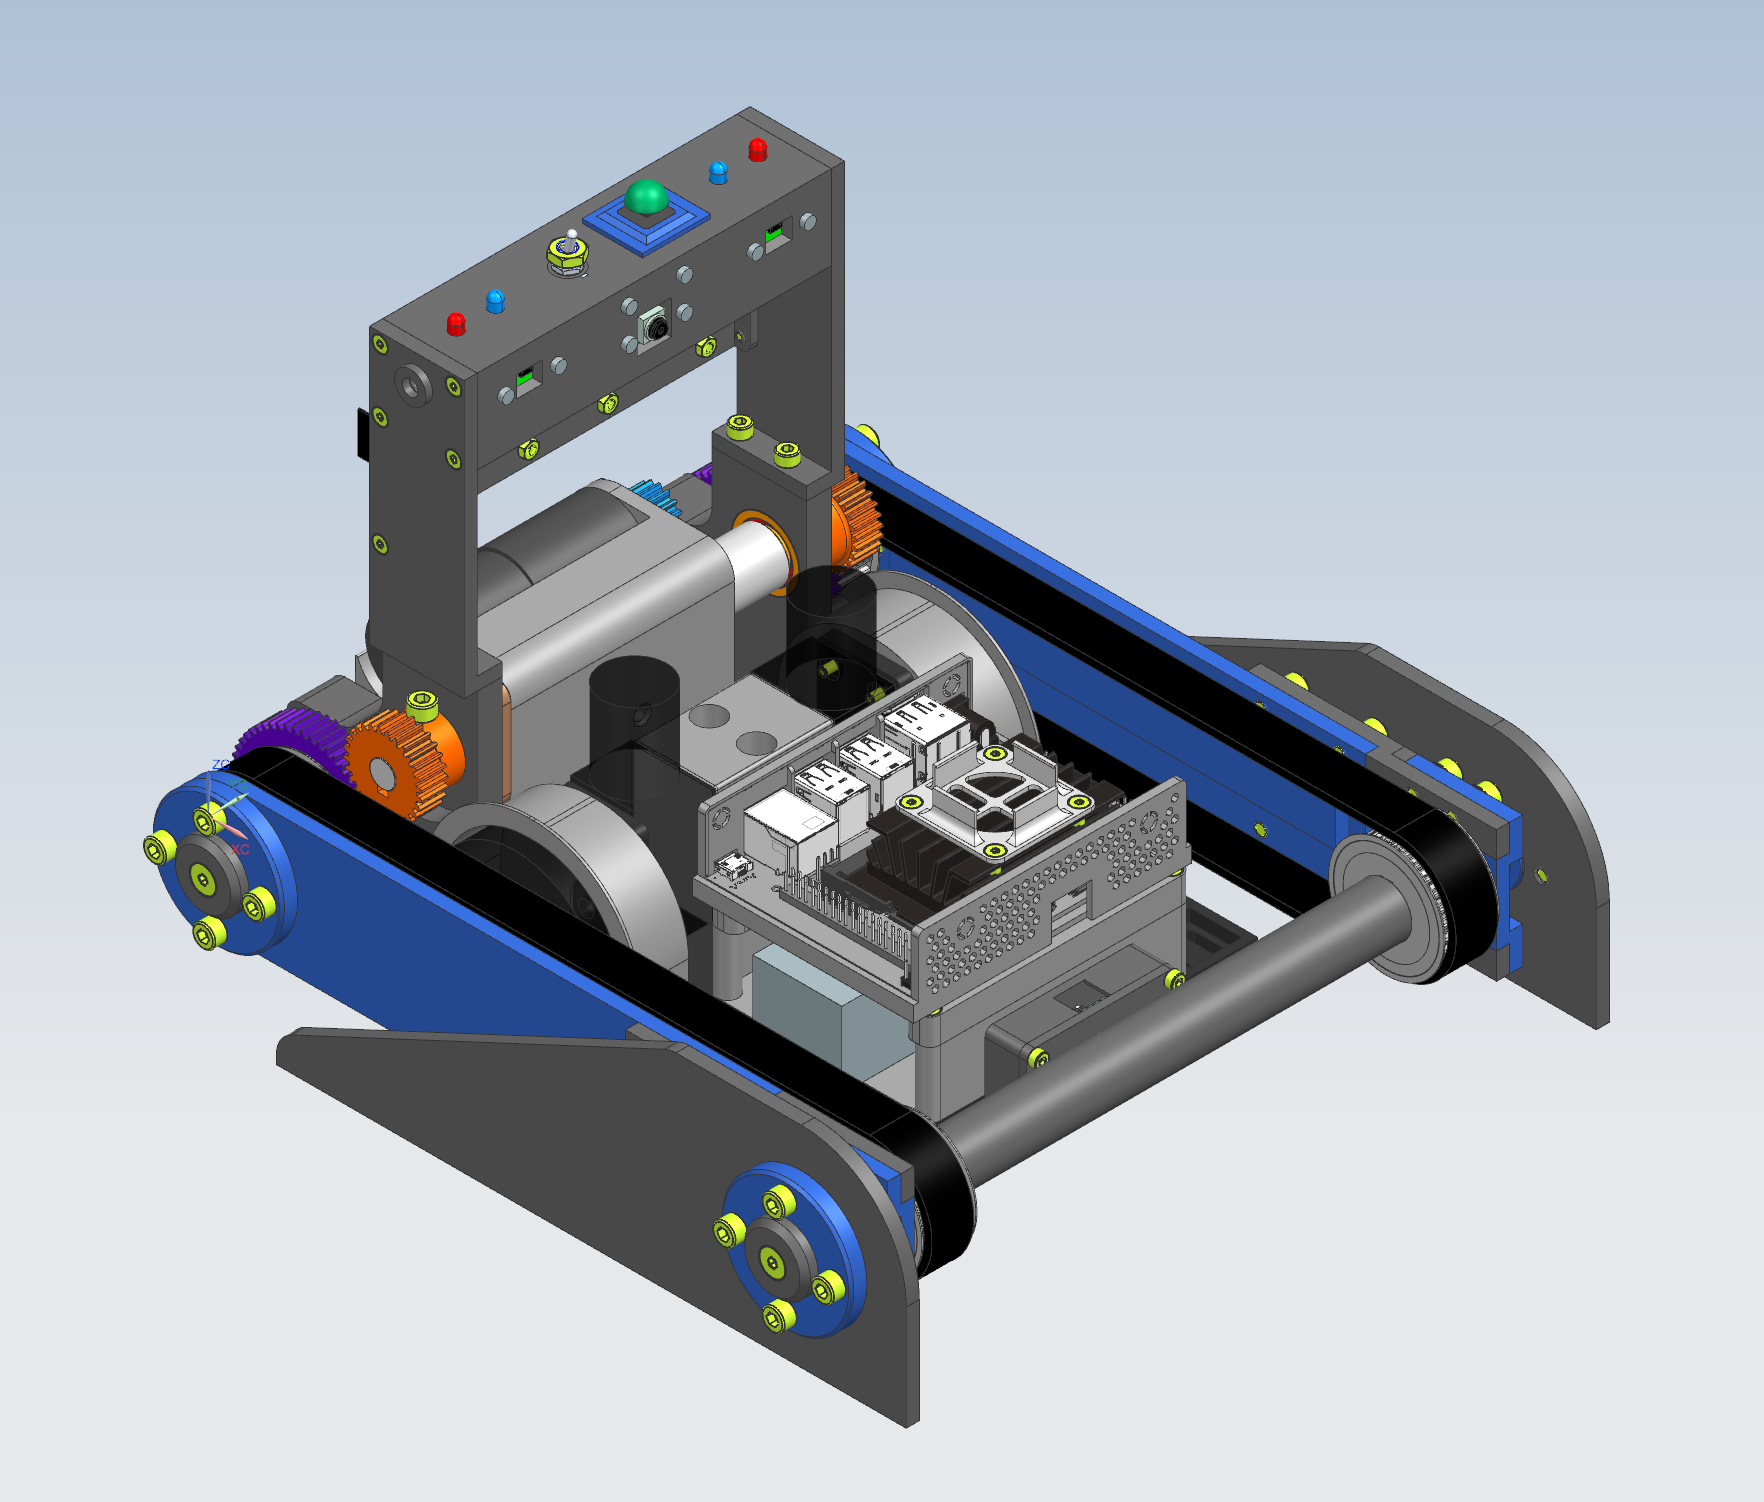
\includegraphics[width=0.9\textwidth]{img/Gerät Aufbau/CADohneHaube1.png}
  \centering
  \caption{CAD-Modell, Ansicht 1}
  \label{fig:CADohneHaube1}
\end{figure}

\begin{figure}[H]
  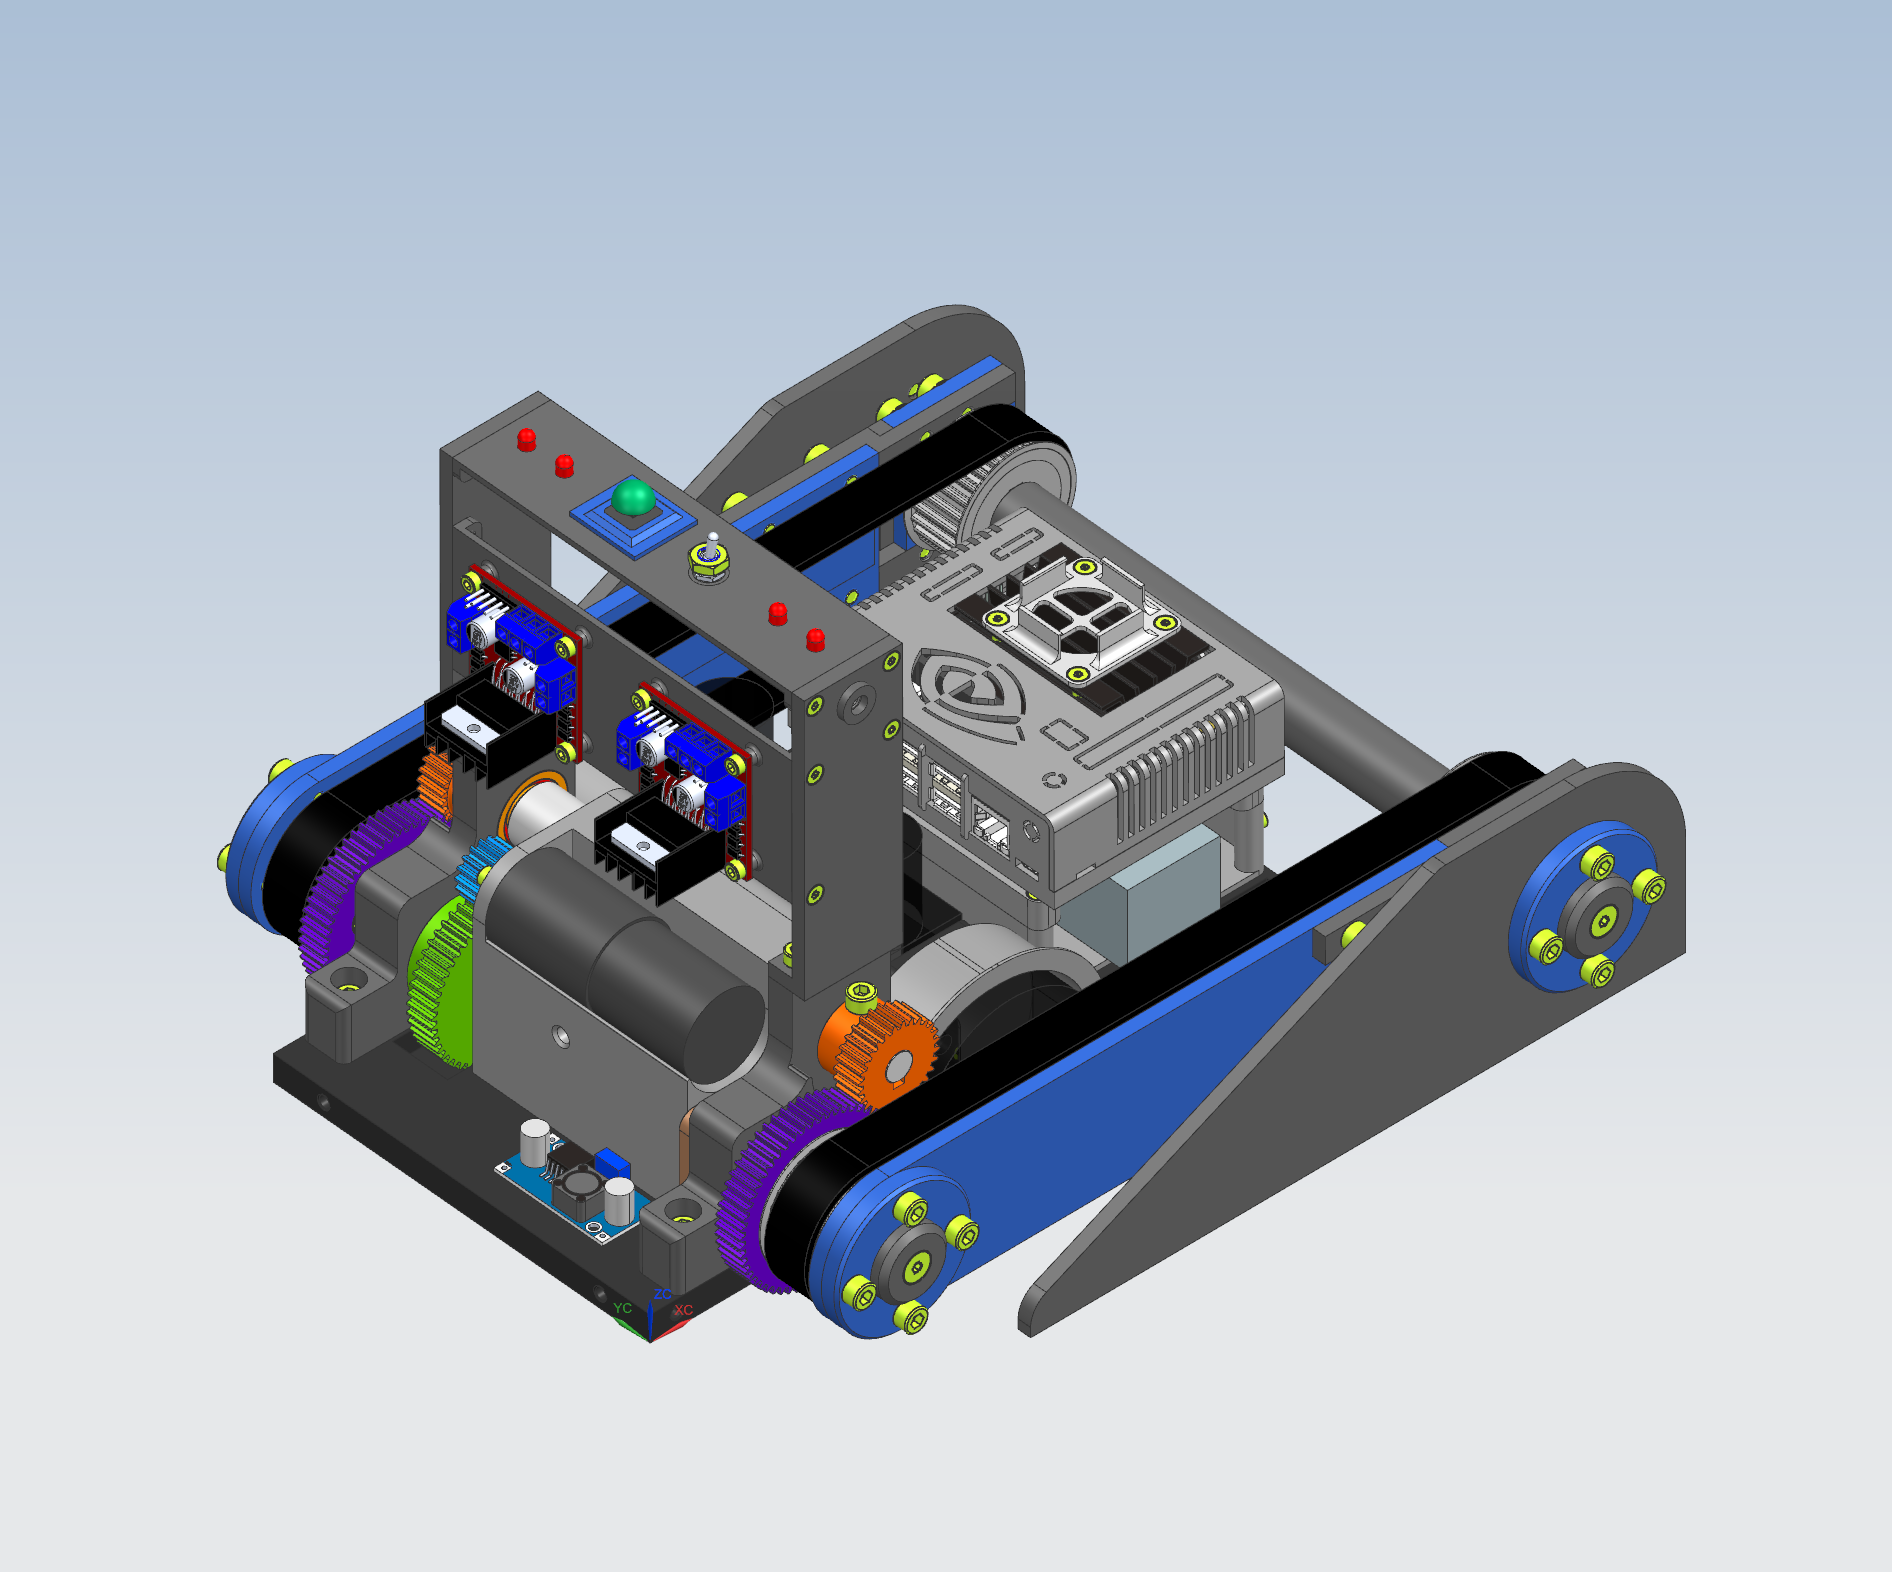
\includegraphics[width=0.9\textwidth]{img/Gerät Aufbau/CADohneHaube2.png}
  \centering
  \caption{CAD-Modell, Ansicht 2}
  \label{fig:CADohneHaube2}
\end{figure}

\newpage

\subsection{Aufgebautes Gerät}

Die Abbildung \ref{fig:GerätohneHaube} zeigt das aufgebaute Gerät ohne Haube und in der Abbildung \ref{fig:GerätmitHaube} ist das Gerät mit Haube zu sehen. 

\begin{figure}[H]
  \includegraphics[width=0.9\textwidth]{img/Gerät Aufbau/GerätohnneHaube.png}
  \centering
  \caption{Gerät ohne Haube}
  \label{fig:GerätohneHaube}
\end{figure}

\begin{figure}[H]
  \includegraphics[width=0.9\textwidth]{img/Gerät Aufbau/GerätmitHaube.png}
  \centering
  \caption{Gerät mit Haube}
  \label{fig:GerätmitHaube}
\end{figure}

\newpage

\subsection{Komponenten}
\label{subsec:Komponenten}

\textbf{Grundplatte:} Die Grundplatte besteht aus zwei 3D-gedruckten Platten, die zusammengeklebt sind. Die notwendigen Bohrungen für Schrauben konnten direkt mitgedruckt werden. Die Halterung für die Fortbewegungsmotoren wurde in die Grundplatte integriert.

\begin{figure}[H]
  \includegraphics[width=0.8\textwidth]{img/Gerät Aufbau/Grundplatte.png}
  \centering
  \caption{Grundplatte}
  \label{fig:Grundplatte}
\end{figure}

\textbf{Wellen:} Die Wellen des Geräts wurden von der mechanischen Werkstatt der Hochschule gefertigt. Sie sind aus Aluminium. Von den 10 Stunden die für die Fertigung in der mechanischen Werkstatt zur Verfügung stehen, wurden 6.5 Stunden für die drei Wellen gebraucht. Die Auslegerwelle wurde jedoch durch eine Kunststoff Welle ersetzt. Dieser Austausch ist im Kapitel \ref{sec:Funktionsweisemit Akku} dokumentiert.

\begin{figure}[H]
  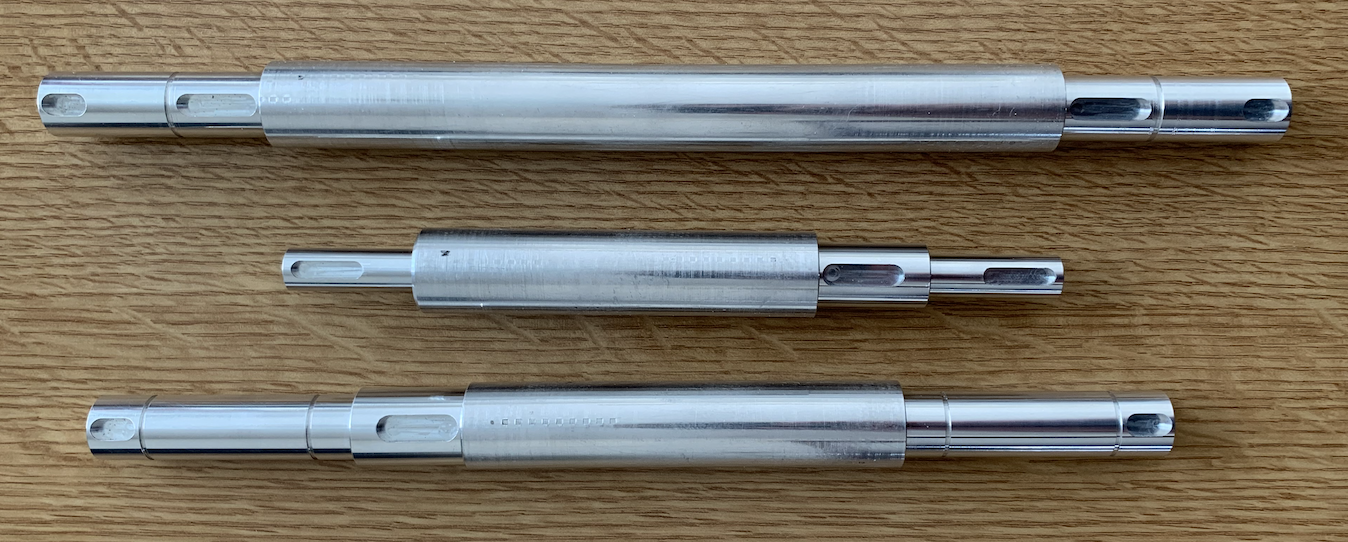
\includegraphics[width=0.8\textwidth]{img/Gerät Aufbau/Wellen.png}
  \centering
  \caption{unten: Welle 1, mitte: Welle 2, oben: Auslegerwelle}
  \label{fig:Wellen}
\end{figure}

\newpage

\textbf{Lagerung der Grundkörperwellen:} An die Grundplatte sind hinten an den Seiten zwei Lagerböcke geschraubt, die die zwei Wellen (Welle 1 und Welle 2), die durch den Grundkörper verlaufen, aufnehmen. Ein Lagerbock ist so gestaltet, dass die zwei Lager fest sind (Festlager) und der andere so, dass sich die Lager im Lagerbock verschieben können (Loslager). Somit sind die Wellen 1 und 2 statisch bestimmt gelagert. Der Festlagerbock ist in der Abbildung \ref{fig:Festlager} zu sehen. Der Loslagerbock ist identisch aufgebaut, nur können sich die Lager axial verschieben.

\begin{figure}[H]
  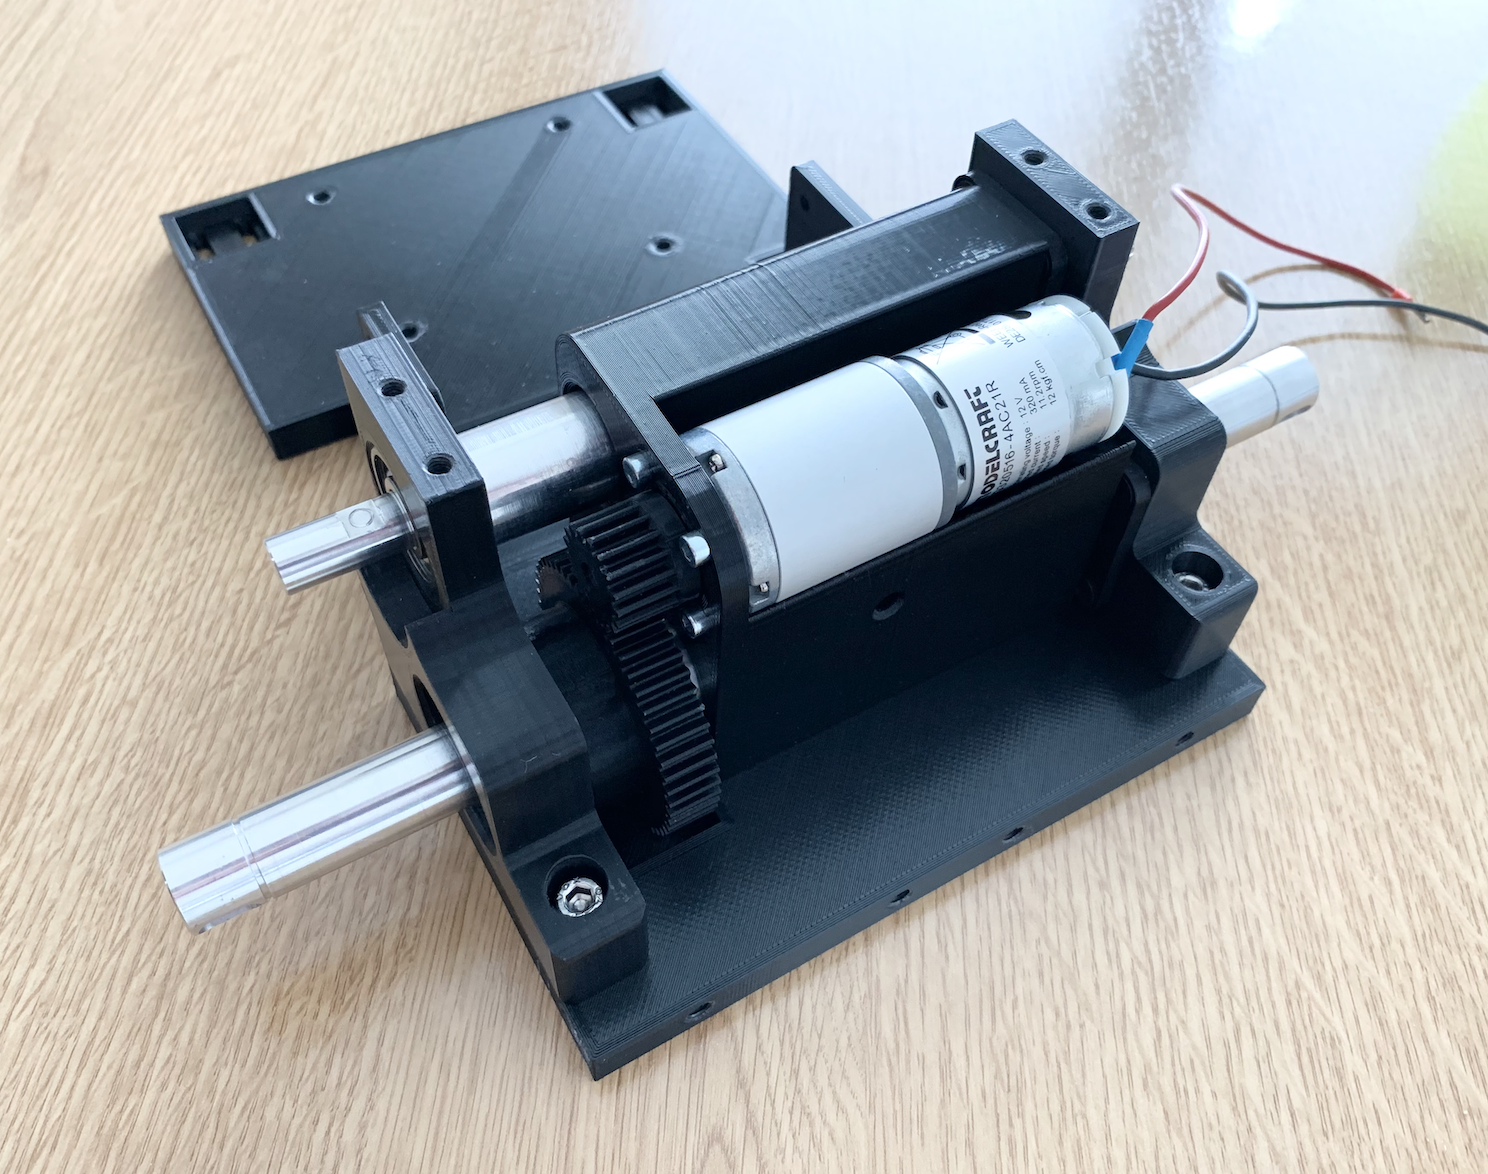
\includegraphics[width=0.7\textwidth]{img/Gerät Aufbau/Lagerböcke.png}
  \centering
  \caption{hinten rechts: Festlager, vorne links: Loslager}
  \label{fig:Lagerung}
\end{figure}

\begin{figure}[H]
  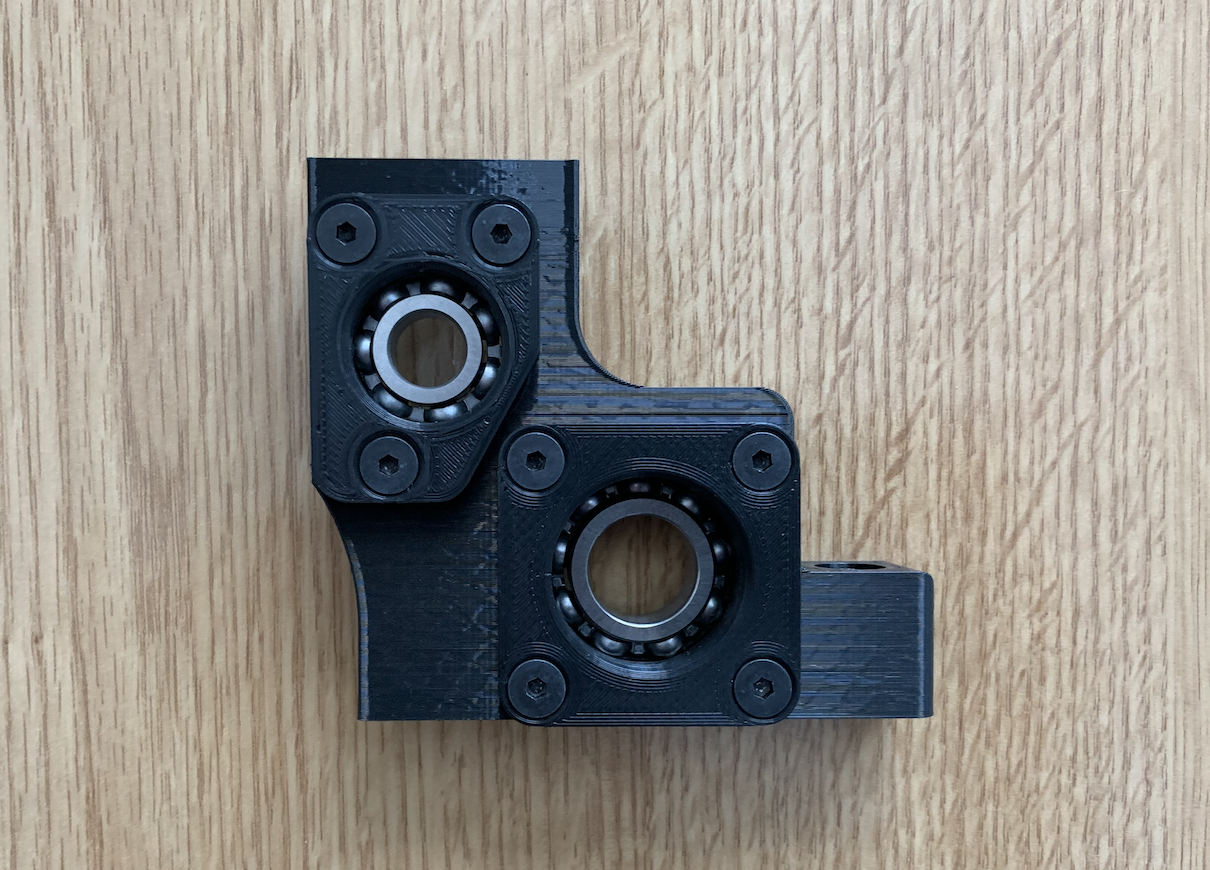
\includegraphics[width=0.6\textwidth]{img/Gerät Aufbau/Festlager.png}
  \centering
  \caption{Lagerbock als Festlager}
  \label{fig:Festlager}
\end{figure}

\newpage

\textbf{Halterung des Hubmotors:} Die Halterung des Hubmotors (siehe Abbildung \ref{fig:Lagerung} ist 3D-gedruckt. Bei der Halterung ist der Motor mit M3-Schrauben befestigt. Zusätzlich liegt der Motor mantelseitig in der Halterungen auf, um den Motor möglichst stabil halten zu können. Die Halterung ist von unten an die Grundplatte geschraubt.

\textbf{Zahnräder:} Alle Zahnräder, die im Gerät verbaut sind, sind 3D-gedruckt. Tests haben gezeigt, dass die Zahnräder die Belastung aushalten. Dies hat die Vorteile , dass zum einen Gewicht und zum anderen Kosten gespart werden können. Das seitliche Gewinde, das die Zahnräder aufweisen, um mit einer Schraube die axiale Verschiebung zu verhindern, ist mit einer eingesetzten Mutter realisiert (siehe Abbildung \ref{fig:Zahnräder}). Dies wird gemacht, damit die Innengewinde eine genügend grosse Festigkeit aufweisen. Die Spezifikationen der Zahnräder sind im Anhang  %\ref{subsec:SpezifikationenZahnrad} 
zu finden.

\begin{figure}[H]
  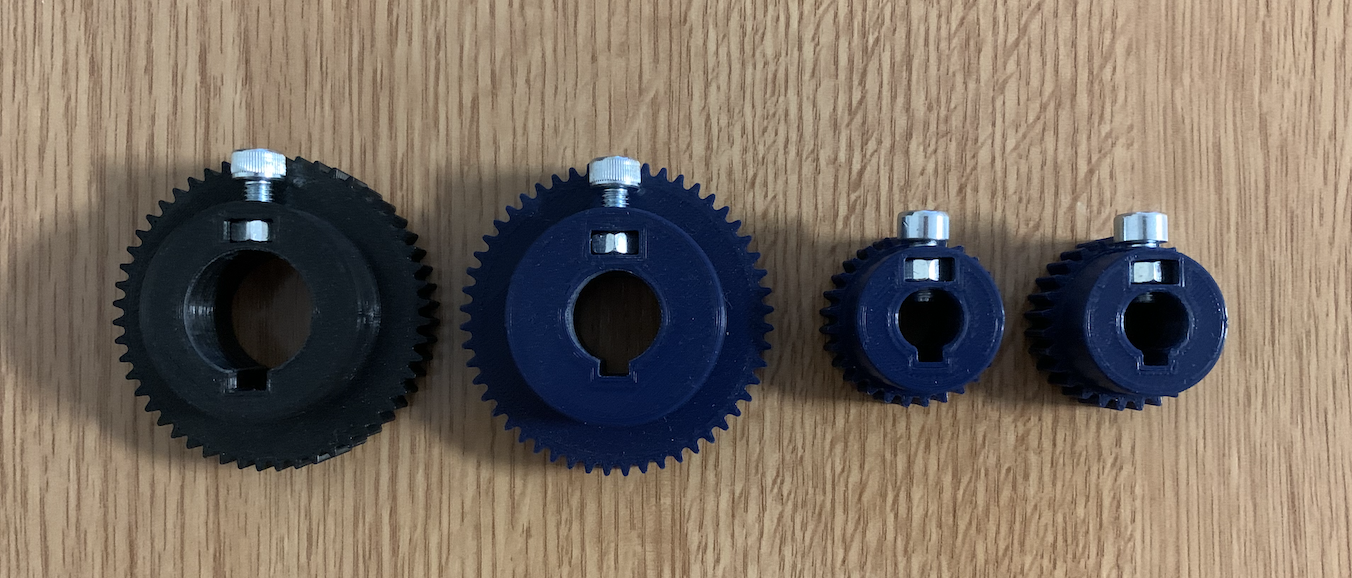
\includegraphics[width=0.9\textwidth]{img/Gerät Aufbau/Zahnräder.png}
  \centering
  \caption{Zahnräder}
  \label{fig:Zahnräder}
\end{figure}

\textbf{Fortbewegung:} Für die Fortbewegung wurden zwei Modellbauräder eingekauft. Die Räder haben einen Durchmesser von 65 mm und sind 32 mm breit. Die Räder sind über ein Verbindungsstück aus Messing mit den Antriebswellen der Fortbewegungsmotoren verbunden. Das Messingstück hat einen Aussensechskant und die Räder einen Innensechskannt. Mit einer Schraube werden die Räder an den Verbindungsstücken gehalten und die Sechskantformverbindung stellt die Mitnahme bei der Drehung sicher. Die Verbindungsstücke sind auf die Motorwellen gesteck und eine seitliche Schraube, die auf die Freifläche der Motorwelle drückt ist für die Mitnahme bei der Drehung zuständig. In der Abbildung \ref{fig:Komponenten der Fortbewegung} sind die Komponenten der Fortbewegung zu sehen und in der Abbildung \ref{fig:Räder an Fortbewegungsmotoren} sind die Räder an die Motoren geschraubt.

\begin{figure}[H]
  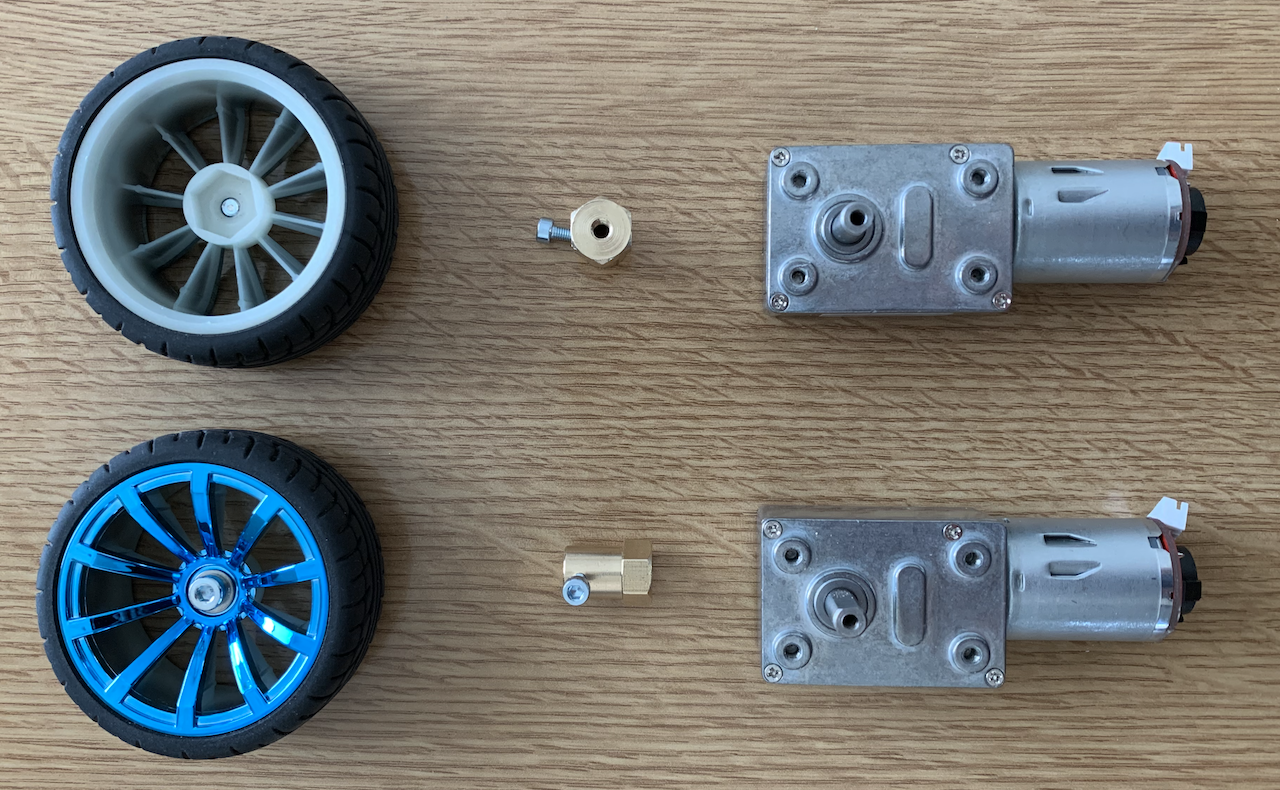
\includegraphics[width=0.8\textwidth]{img/Gerät Aufbau/Räder zerlegt.png}
  \centering
  \caption{Komponenten der Fortbewegung}
  \label{fig:Komponenten der Fortbewegung}
\end{figure}

\begin{figure}[H]
  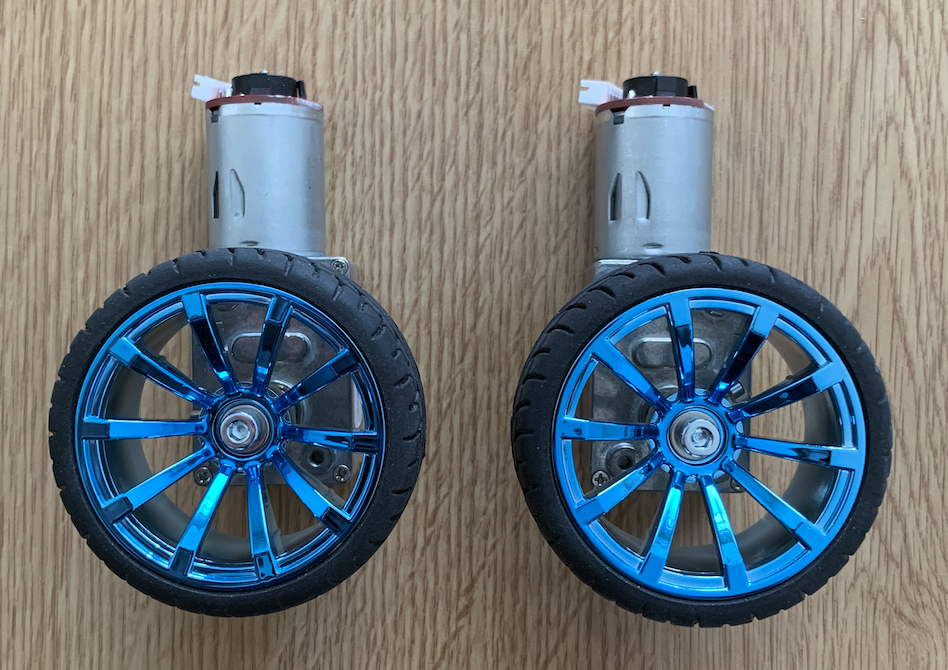
\includegraphics[width=0.8\textwidth]{img/Gerät Aufbau/Räder mit Motor.png}
  \centering
  \caption{Räder an Fortbewegungsmotoren}
  \label{fig:Räder an Fortbewegungsmotoren}
\end{figure}

\newpage

\textbf{Ausleger:} Die seitlichen zwei Ausleger bestehen jeweils aus einer Verbindungsleiste und einem Standfuss. Sie sind über die Auslegerwelle miteinander verbunden.

\begin{figure}[H]
  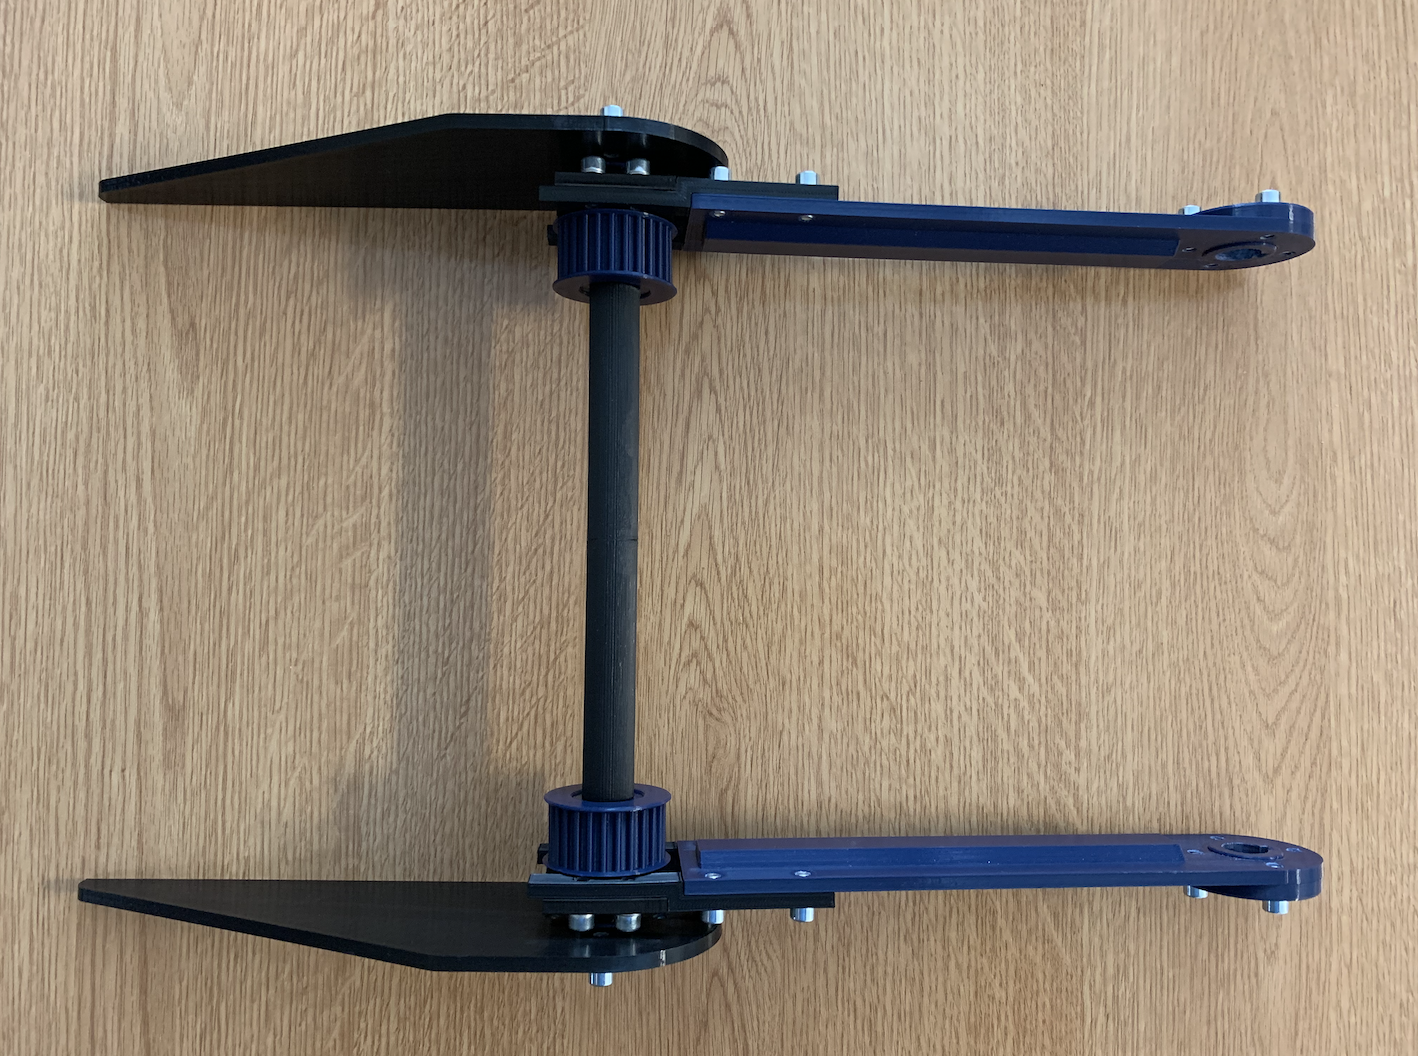
\includegraphics[width=0.8\textwidth]{img/Gerät Aufbau/Ausleger.png}
  \centering
  \caption{Ausleger}
  \label{fig:Ausleger}
\end{figure}

\textbf{Verbindungsleisten:} Die Verbindungsleisten bestehen aus einer Leiste, einem angeschraubten Flansch und angeschraubten Führungen. Die Komponenten der Verbindungsleisten sind 3D-gedruckt.

\begin{figure}[H]
  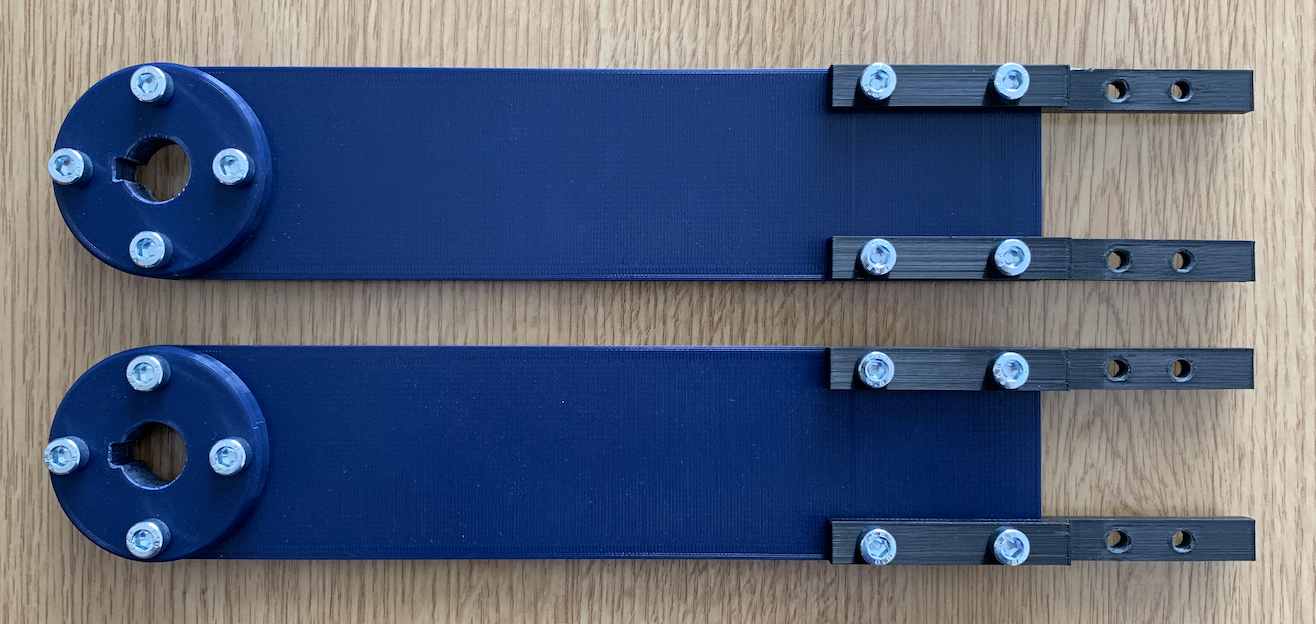
\includegraphics[width=0.8\textwidth]{img/Gerät Aufbau/Verbindungsleisten.png}
  \centering
  \caption{Verbindungsleisten mit angeschraubten Flanschen}
  \label{fig:Verbindungsleisten}
\end{figure}

\textbf{Standfüsse:} Die Standfüsse bestehen aus einem Blech und einem angeschraubten Flansch. Der Flansch ist identisch wie dieser, der bei den Verbindungsleisten eingesetzt ist. Die Standfüsse sind 3D-gedruckt.

\begin{figure}[H]
  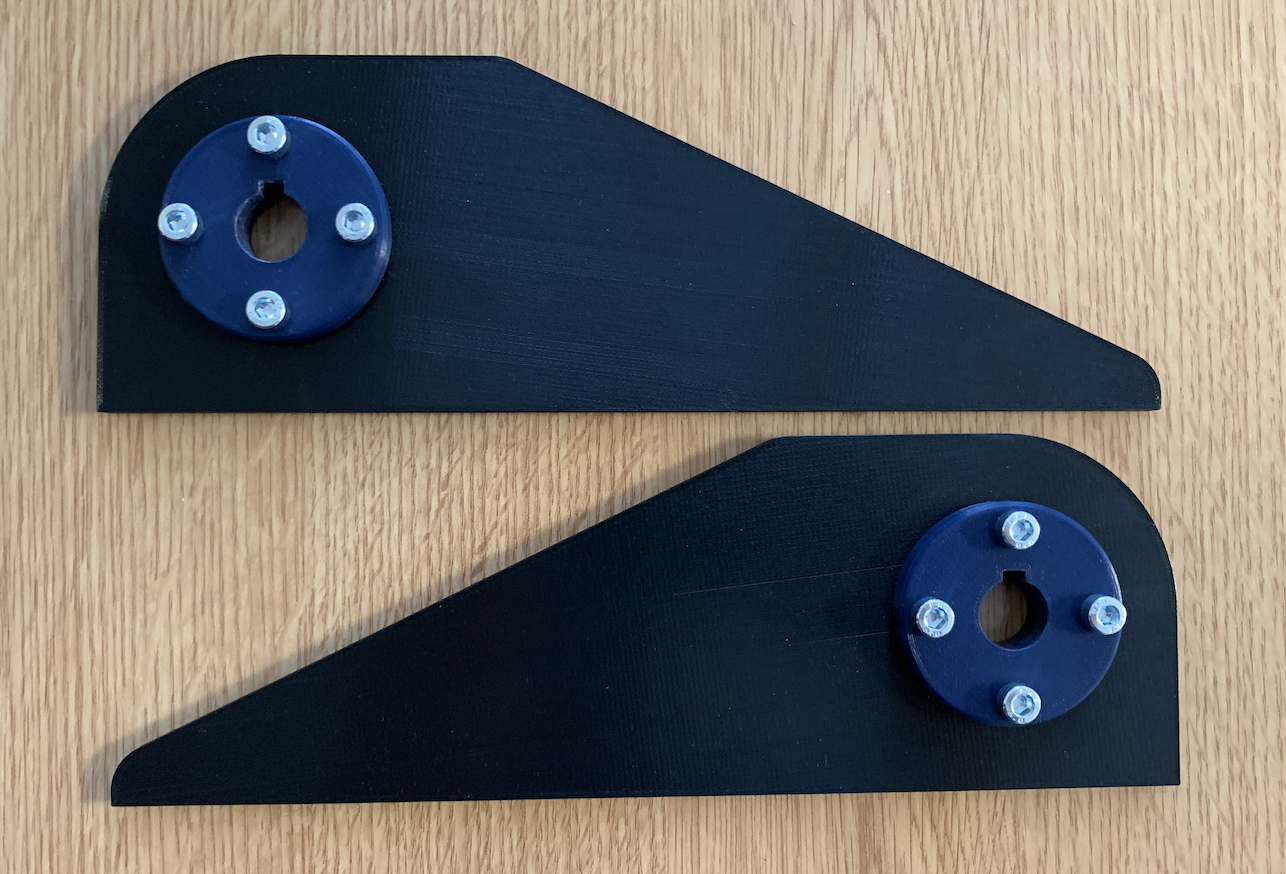
\includegraphics[width=0.8\textwidth]{img/Gerät Aufbau/Standfüsse.png}
  \centering
  \caption{Standfüsse}
  \label{fig:Standfüsse}
\end{figure}

\newpage

\textbf{Auslegerwelle:} Auf der Auslegerwelle (siehe Abbildung \ref{fig:Auslegerwelle}), die 3D-gedruckt ist, sind auf beiden Seiten die Abtriebsräder der Zahnriemen aufgesteckt. Sie besitzen eine Passfederverbindung. Weiter sind die Aufnahmestücke der Verbindungsleisten, die drehbar auf der Welle sitzen aufgesteckt. Diese Aufnahmestücke enthalten in der Mitte ein Lager, was in der Abbildung \ref{fig:Aufnahmestück} zu sehen ist.

\begin{figure}[H]
  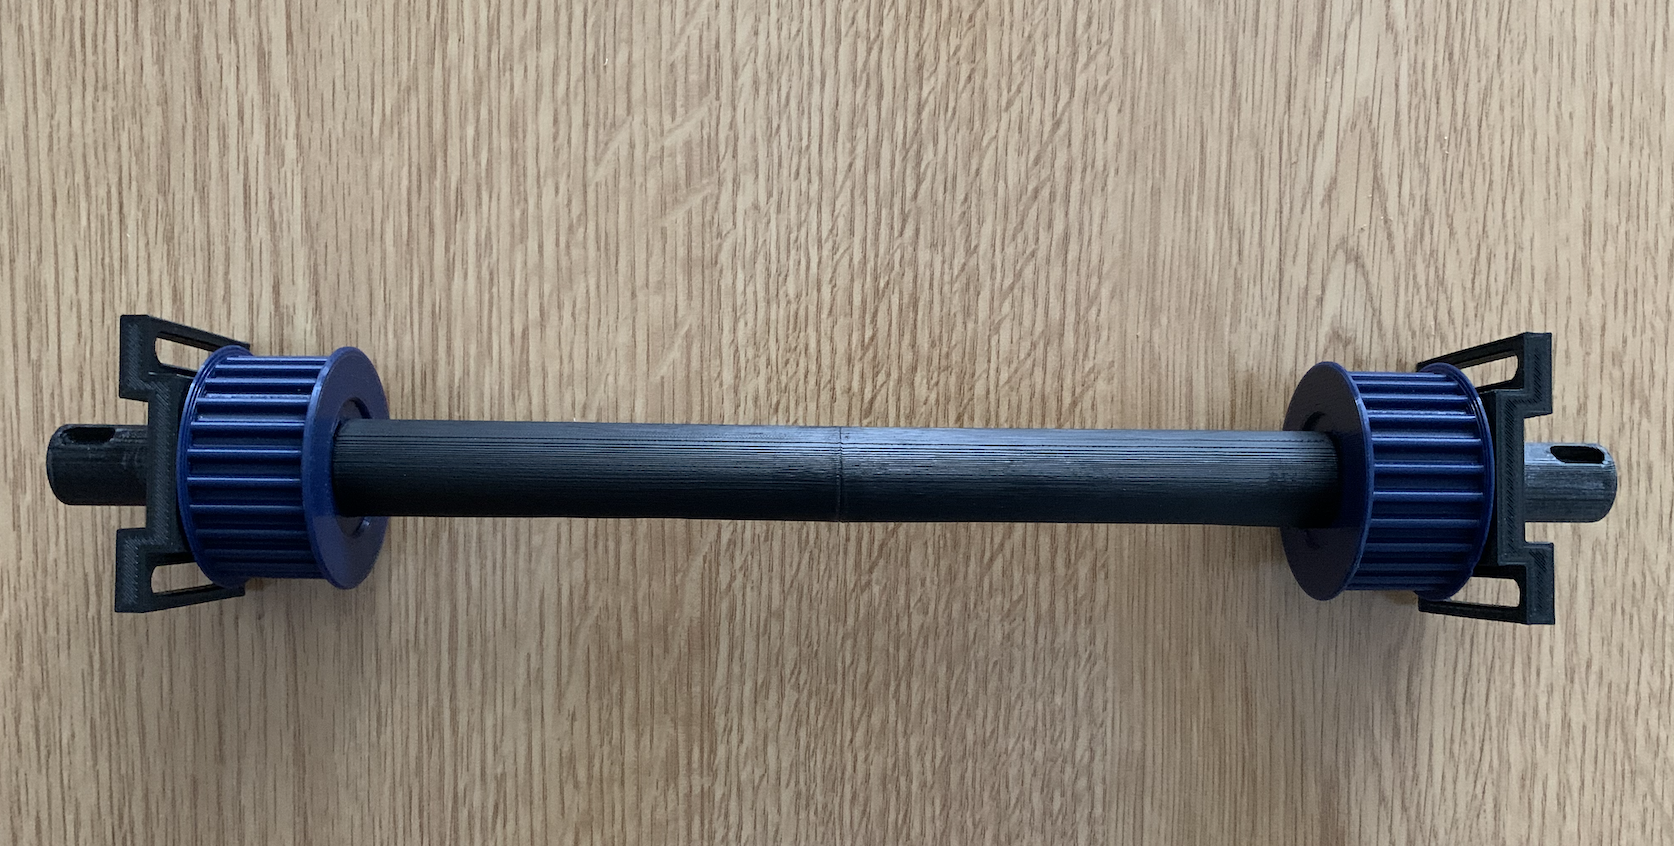
\includegraphics[width=0.8\textwidth]{img/Gerät Aufbau/Auslegerwelle.png}
  \centering
  \caption{Auslegerwelle}
  \label{fig:Auslegerwelle}
\end{figure}

\begin{figure}[H]
  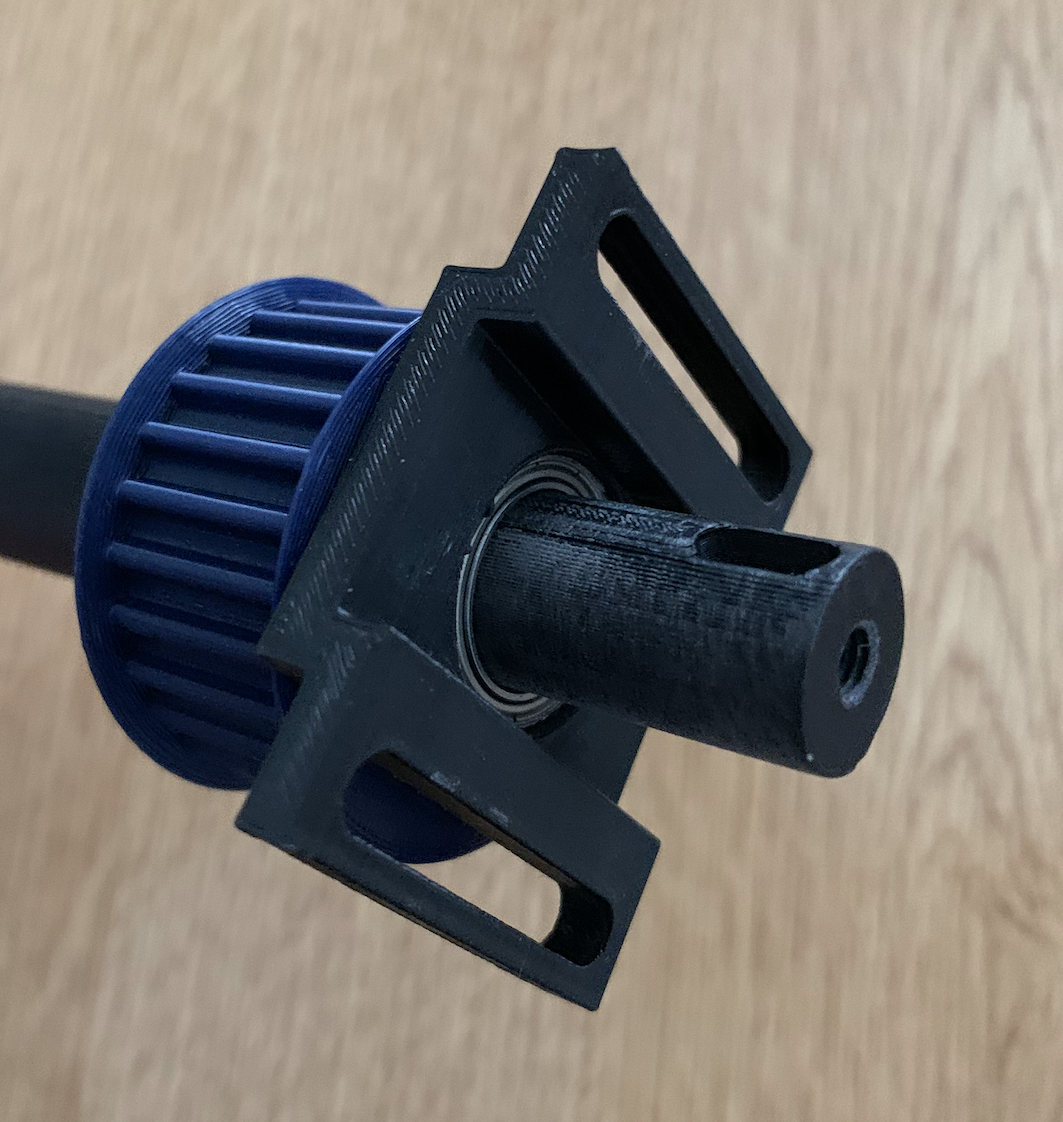
\includegraphics[width=0.5\textwidth]{img/Gerät Aufbau/Aufnahmestück.png}
  \centering
  \caption{Auslegerwelle-Aufnahmestück}
  \label{fig:Aufnahmestück}
\end{figure}

\newpage

\textbf{Zahnriementrieb:} Die Zahnriemen sind auf beiden Seiten des Geräts zwischen der Welle 1 und der Auslegerwelle gespannt. Das treibende Zahnriemenrad sitzt drehbar auf der Welle 1 und das getriebene Zahnriemenrad ist auf der Auslegerwelle fixiert. Die Spezifikationen zu den Zahnriemen sind im Anhang  %\ref{subsec:SpezifikationenZahnriemen} 
zu finden.

\begin{figure}[H]
  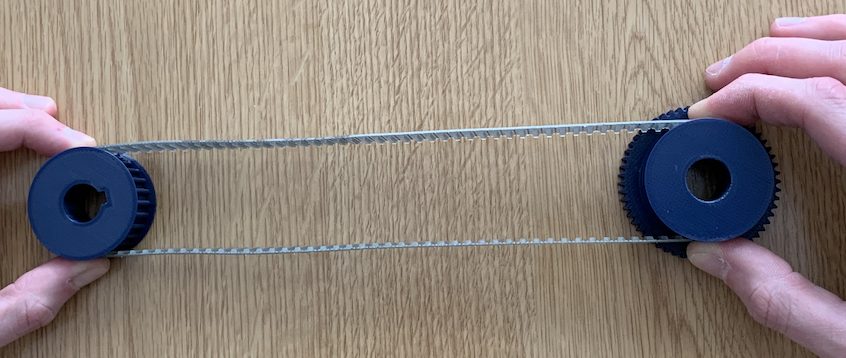
\includegraphics[width=0.8\textwidth]{img/Gerät Aufbau/Zahnriementrieb.png}
  \centering
  \caption{Zahnriementrieb}
  \label{fig:Zahnriementrieb}
\end{figure}

Die Zahnriemen, sind mithilfe eines Einlegestücks gespannt. Diese Methode zum Spannen der Zahnriemen wurde experimentell getestet. Es stellte sich heraus, dass die Spannung, die so erreicht werden kann, ausreicht.

\begin{figure}[H]
  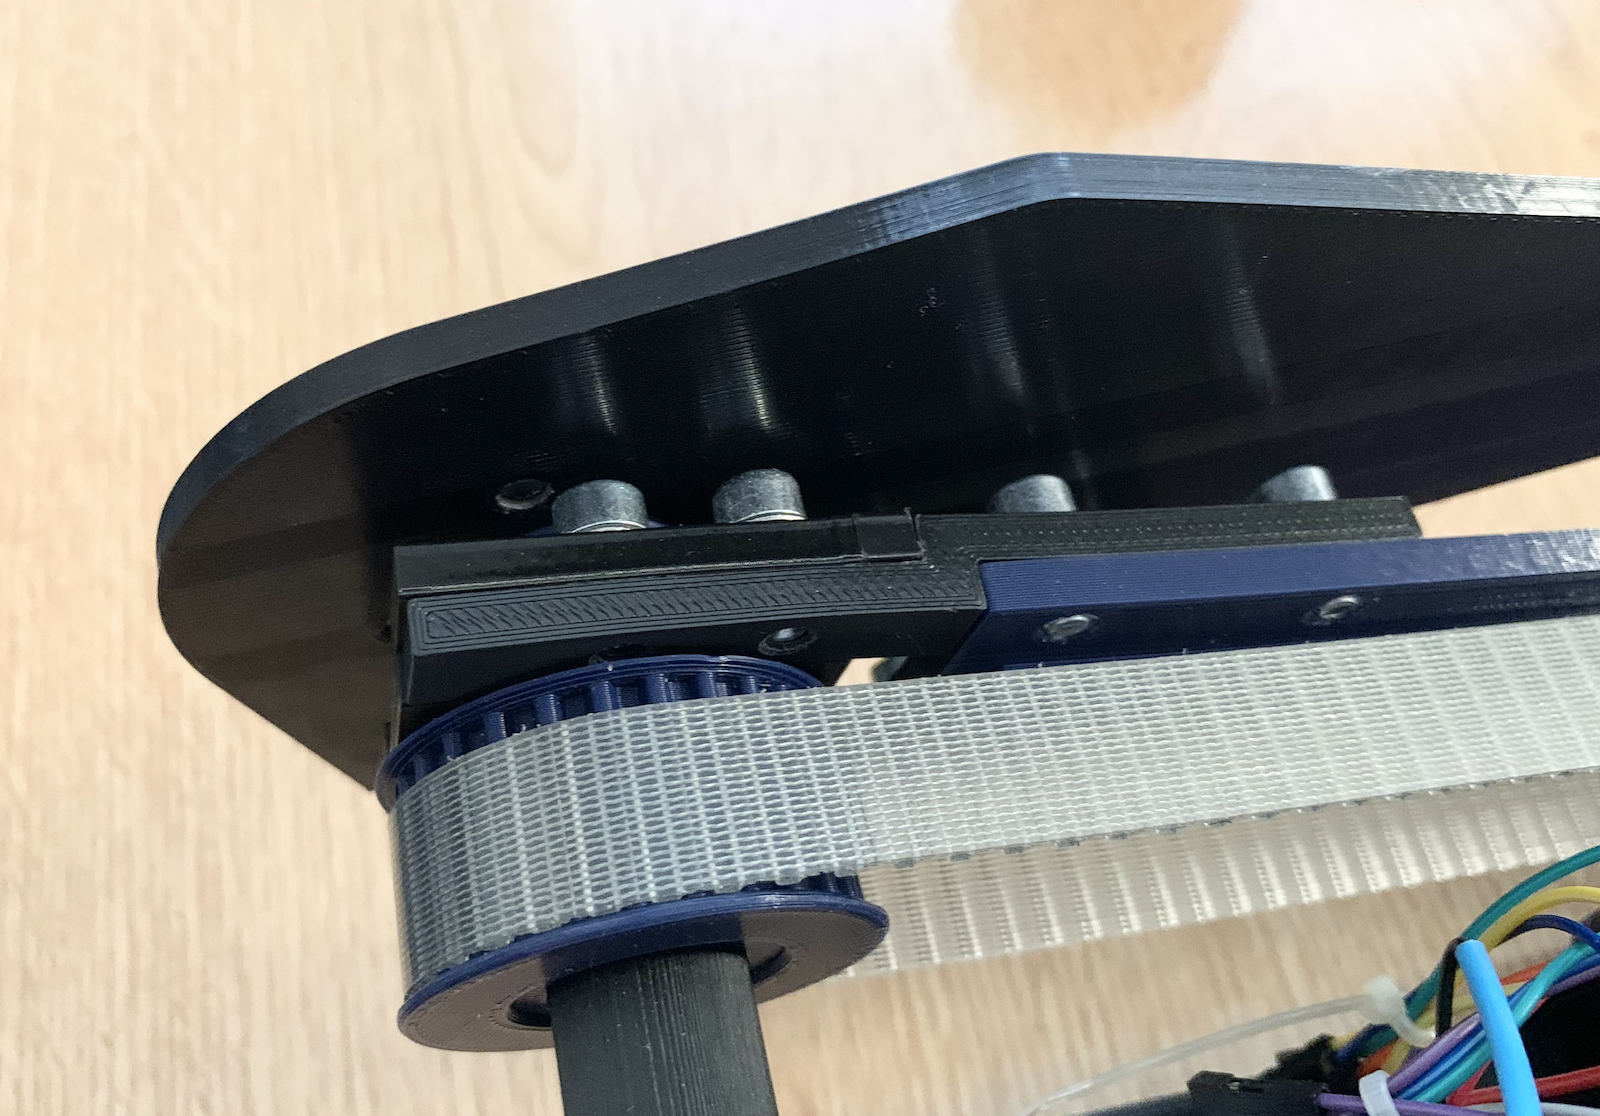
\includegraphics[width=0.8\textwidth]{img/Gerät Aufbau/Zahnriemenspanner.png}
  \centering
  \caption{Methode zum Spannen der Zahnriemen}
  \label{fig:Methode zum Spannen}
\end{figure}

\newpage




\textbf{Akkugehäuse und Bordhalterung:} Der Akku, der die Energiequelle des Geräts ist, ist in einem Gehäuse direkt auf der Grundplatte montiert. Das Gehäuse für das Jetson-Bord ist auf dem Akkugehäuse befestigt. Für die Kühlung des Boards wird ein Ventilator verwendet, für dessen Montage ein Adapter konstruiert und gedruckt wurde.

\begin{figure}[H]
  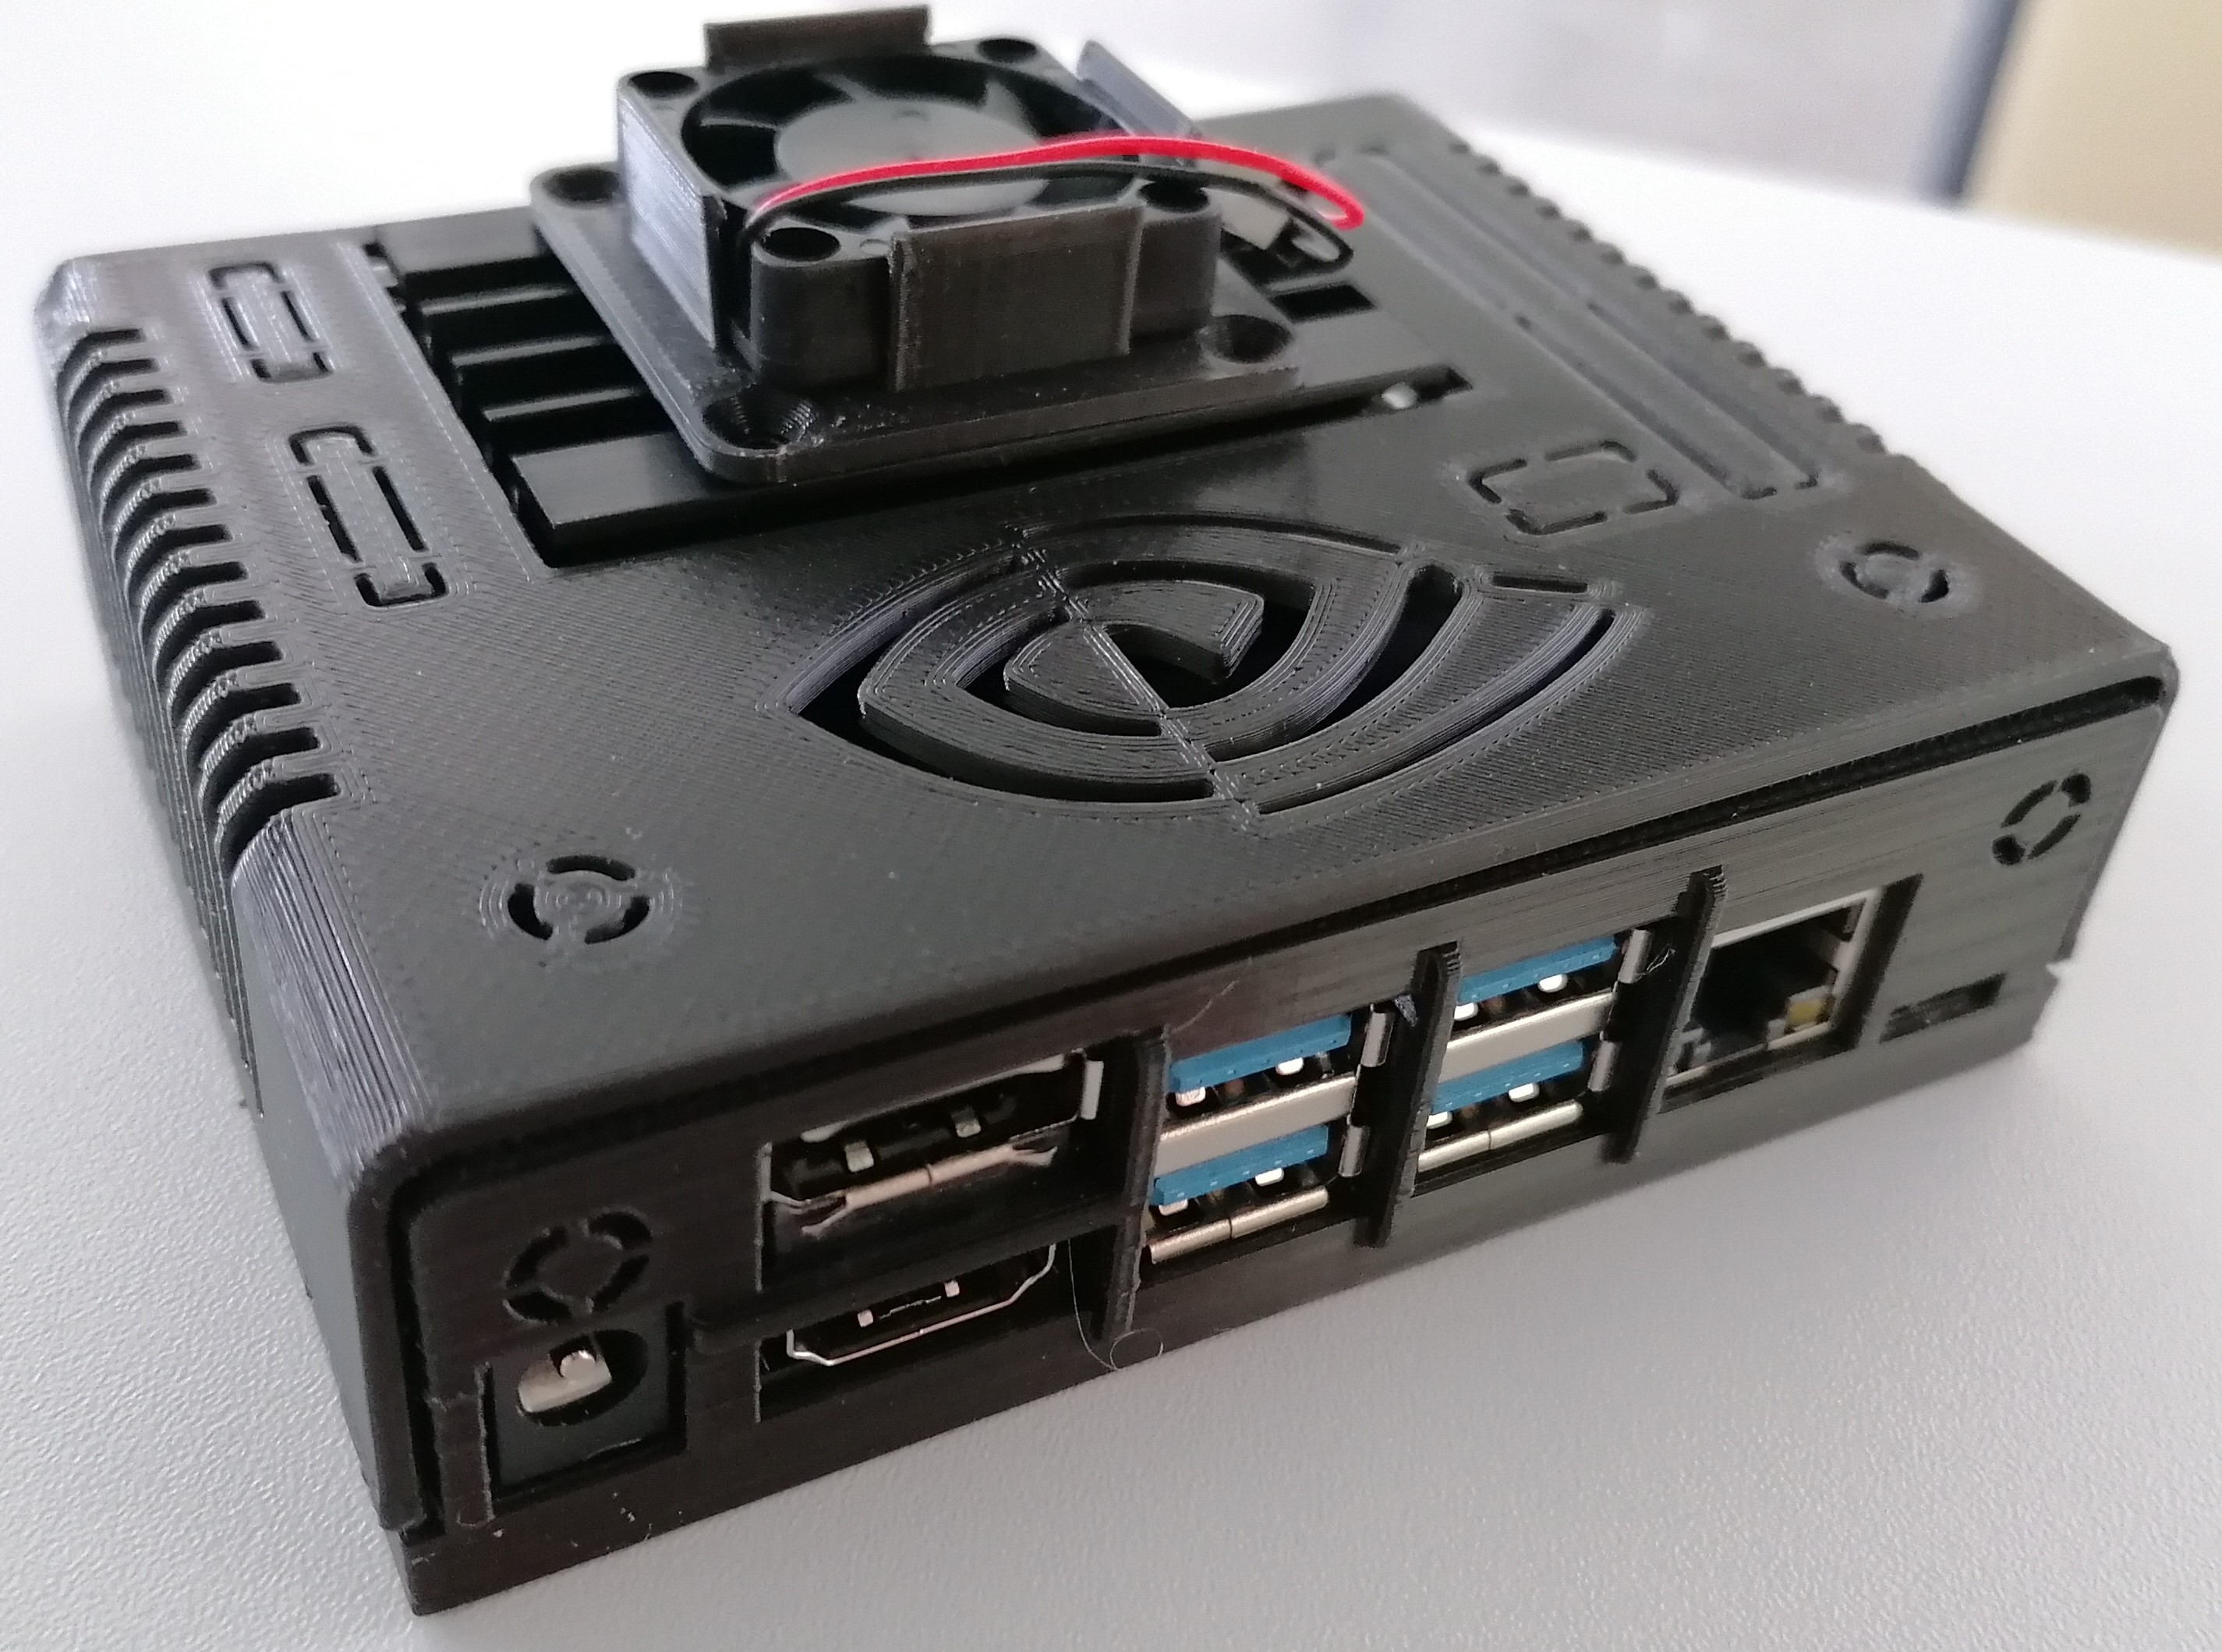
\includegraphics[width=0.8\textwidth]{img/Gerät Aufbau/Gehäuse_Jetson_2.jpeg.jpg}
  \centering
  \caption{Akkugehäuse und Bordhalterung}
  \label{fig:Akkugehäuse und Bordhalterung}
\end{figure}

\newpage

\textbf{Kamera- und TOF-Sensorenhalterung:} Die Halterung für die Kamera und die TOF-Sensoren ist auf die Lagerböcke geschraubt. Die Komponenten der Halterung sind 3D-gedruckt. Die Kamera und die TOF-Sensoren sind von innen an die Halterung geschraubt. Weiter sind oben an dieser Halterung der Startknopf, der NOTAUS-Schalter und vier LED`s angebracht. Auf der Rückseite der Halterung sind die zwei H-Brücken und der Multiplexer angeschraubt.

\begin{figure}[H]
  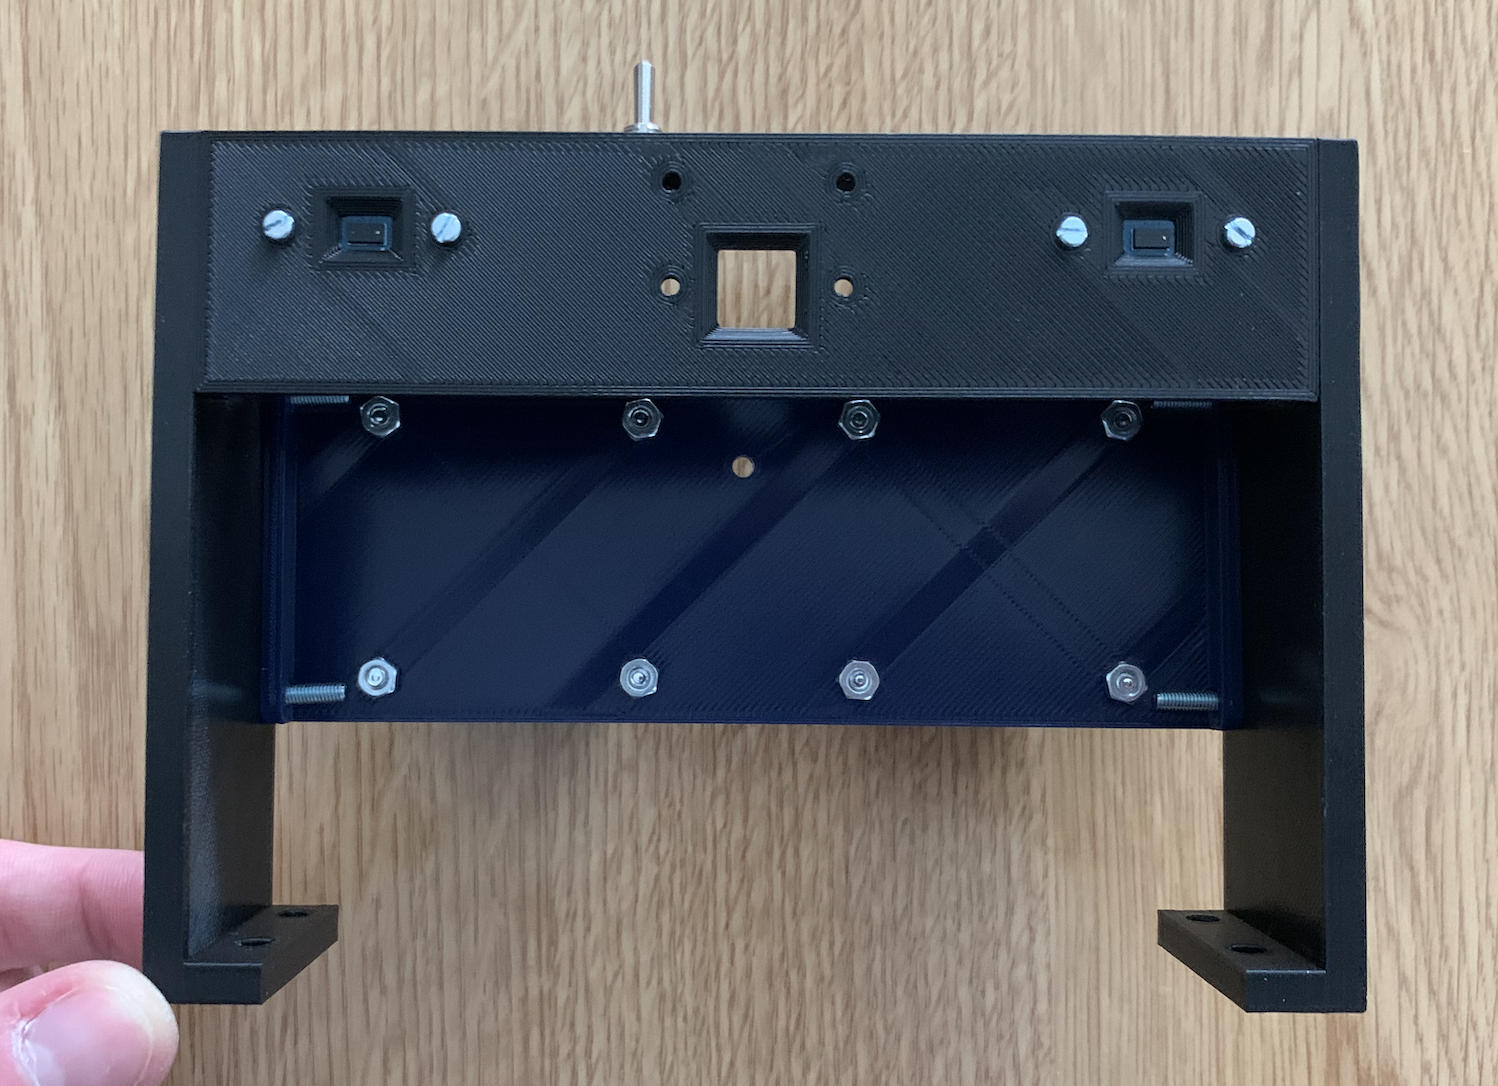
\includegraphics[width=0.8\textwidth]{img/Gerät Aufbau/Kameraturmseite.png}
  \centering
  \caption{Kamera- und TOF-Sensorenhalterung von vorne}
  \label{fig:Kameraturnseite}
\end{figure}

\begin{figure}[H]
  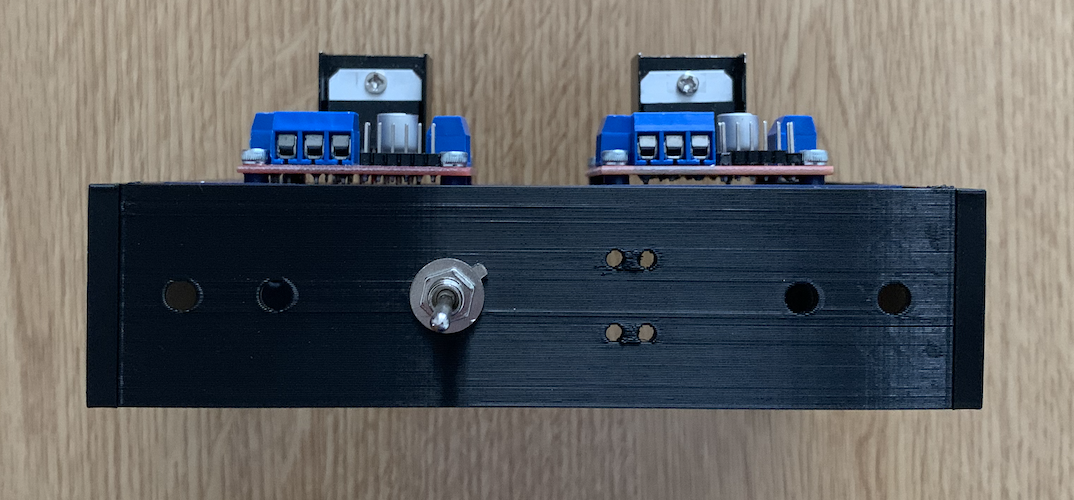
\includegraphics[width=0.8\textwidth]{img/Gerät Aufbau/Kameraturmoben.png}
  \centering
  \caption{Kamera- und TOF-Sensorenhalterung von oben}
  \label{fig:Kameraturmoben}
\end{figure}

\newpage

\textbf{Ultraschallsensorhalterung:} Der Ultraschallsensor ist in einer 3D-gedruckten Halterung an der Grundplatte angeschraubt.

\begin{figure}[H]
  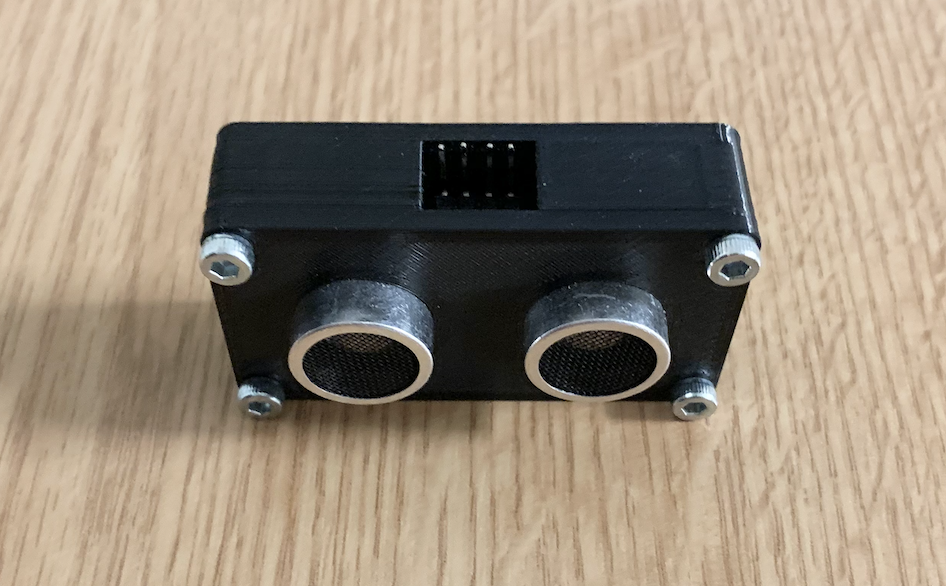
\includegraphics[width=0.6\textwidth]{img/Gerät Aufbau/Usensorhalterung.png}
  \centering
  \caption{Ultraschallsensorhalterung}
  \label{fig:Uschallsensorhalterung}
\end{figure}

\textbf{Halbkugelstützen:} Die Halbkugelstützen erfüllen zwei Funktionen. Auf der einen Seite halten sie den Roboter gerade während der Fortbewegung, auf der anderen Seite geben die Stützen, welche auf Drucksensoren montiert sind, das Signal für den Bodenkontakt.

\begin{figure}[H]
  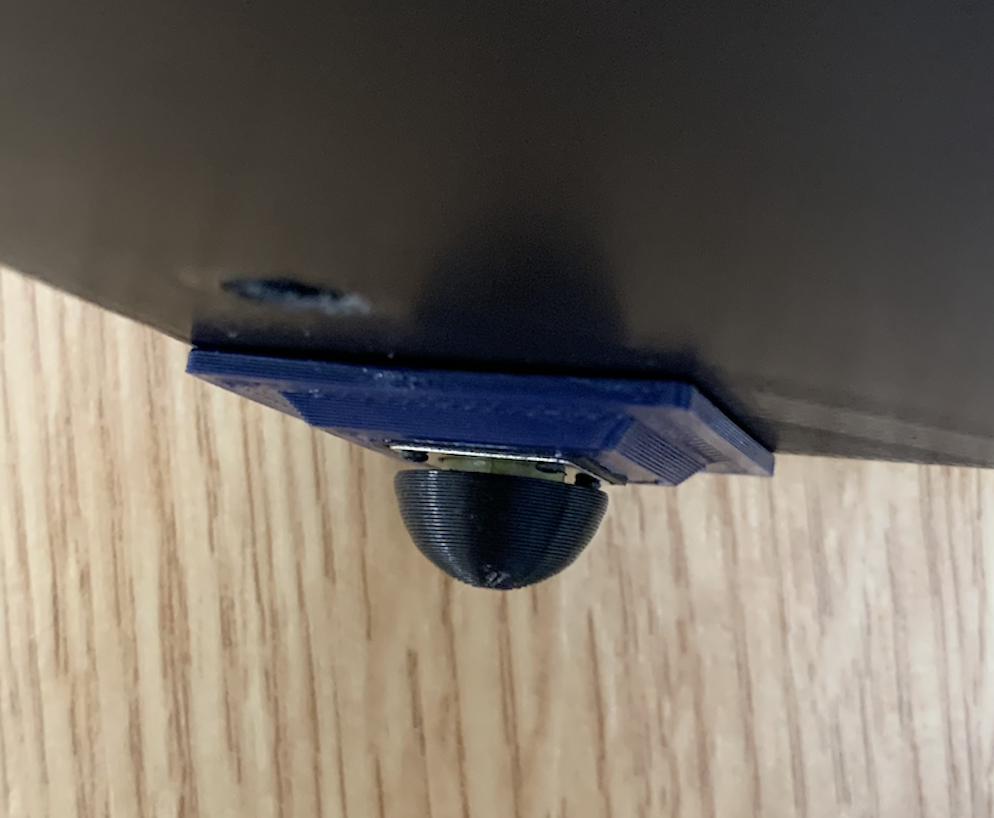
\includegraphics[width=0.6\textwidth]{img/Gerät Aufbau/Halbkugel.png}
  \centering
  \caption{Halbkugelstütze}
  \label{fig:Halbkugelstütze}
\end{figure}

\newpage

\textbf{Haube:}

Das Gerät wird von einer Haube geschützt. Diese Haube lässt sich von oben über den Grundkörper schieben und wird mit Schrauben an die Grundplatte geschraubt. Die Haube wurde aus mehreren 3D-gedruckten dünnen Platten zusammengeklebt. So konnte die Haube dünn und leicht gebaut werden.

\begin{figure}[H]
  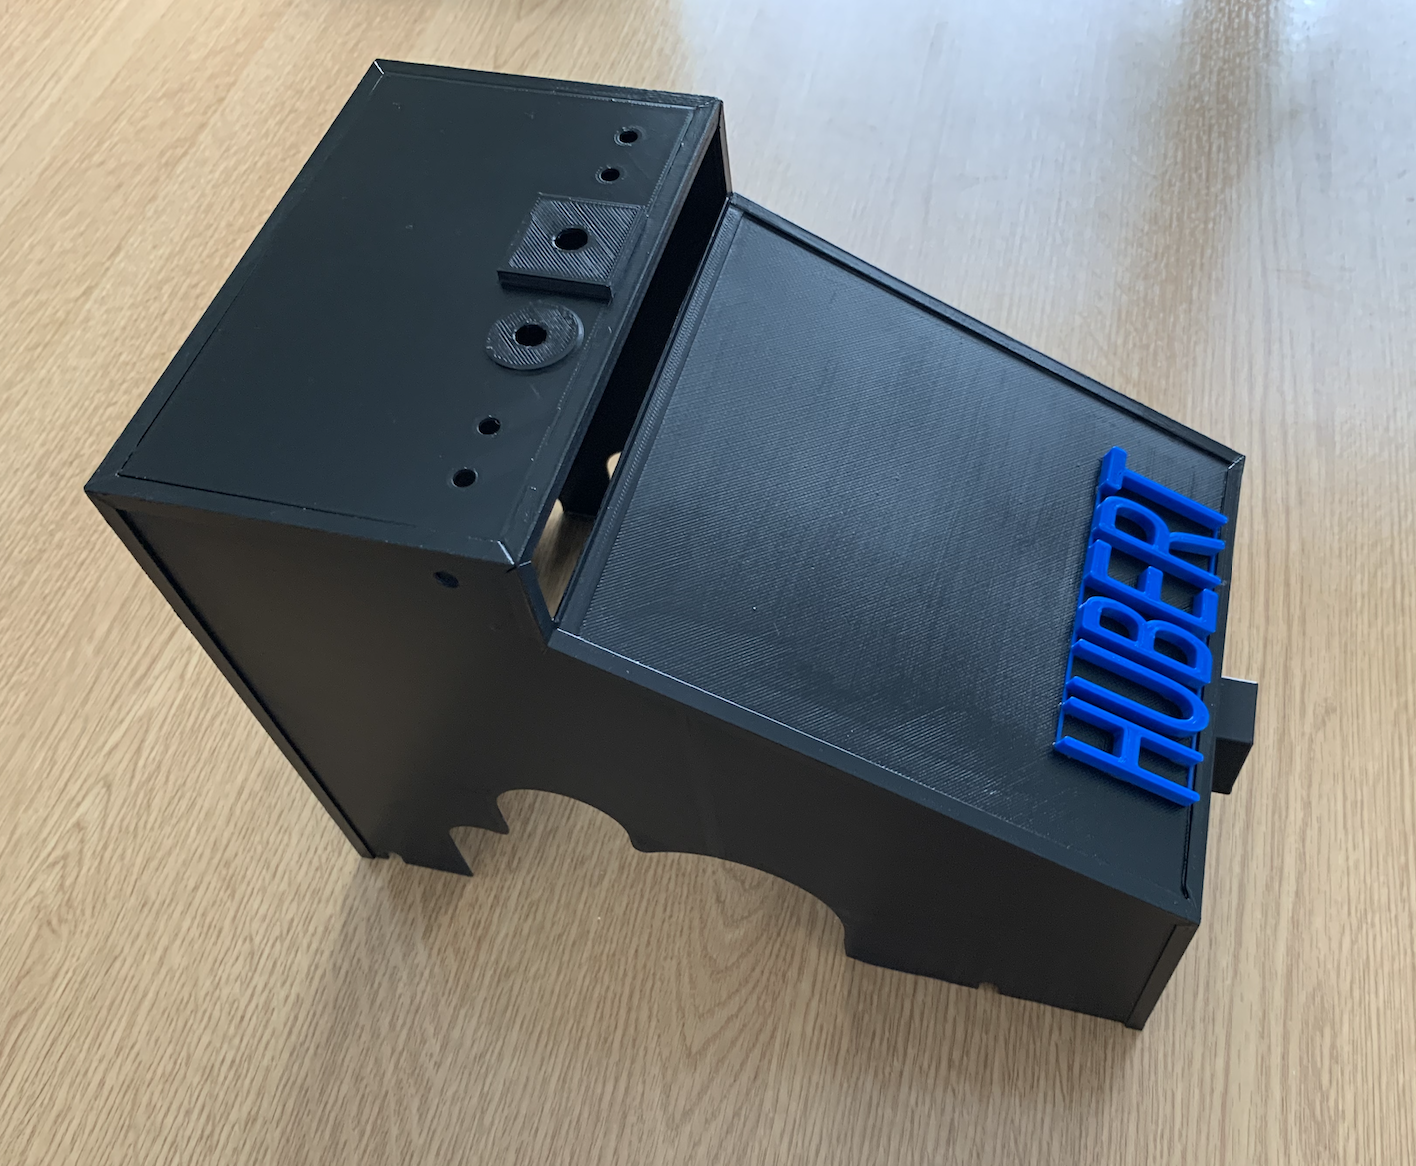
\includegraphics[width=0.8\textwidth]{img/Gerät Aufbau/Haube.png}
  \centering
  \caption{Haube des Grundkörpers}
  \label{fig:Haube}
\end{figure}






\newpage

\subsection{Elektronikkomponenten}
\subsection{Pinbelegung}
Die Abbildung \ref{fig:pinout-raspi} zeigt die Pinbelegung des Jetson. Am Nvidia Jetson Nano sind folgende Komponenten angeschlossen:

\begin{itemize}
    \item zwei TOF-Sensoren via Multiplexer
    \item ein \acrshort{i2c}-PWM-Board für die PWM-Signale für die H-Brücken 
    \item ein Ultraschallsensor
    \item zwei Taster für den Grundkörper und ein Starttaster
    \item zwei H-Brücken für Fortbewegung/Treppensteigen
    \item zwei Encoder für je ein Motor der Fortbewegung
    \item vier LEDs für Bestätigung
\end{itemize} 

\begin{figure}[H]
  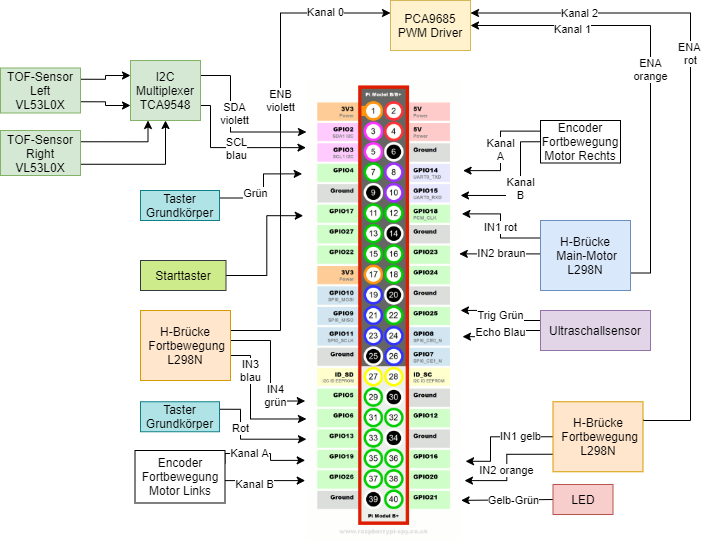
\includegraphics[width=0.9\textwidth]{img/Elektronik/pinout_raspi_ohne_expander.png}
  \centering
  \caption{Pinbelegung des Jetson Nano}
  \label{fig:pinout-raspi}
\end{figure}


\newpage
\subsection{TOF-Sensoren}
Für die Ausrichtung des Roboters werden zwei TOF-Sensoren verwendet, welche die Abstände zur Treppenkante messen. Die TOF-Sensoren senden die Daten über \acrshort{i2c} an den Controller. Da die Sensoren von Werk aus die gleiche Adresse verwenden, muss diese angepasst werden. Dabei gibt es zwei Möglichkeiten:
\begin{enumerate}
    \item Durch verbinden des Xshut-Pins des Vl53L0X-Chips mit Ground, kann die Adresse verändert werden. Der Nachteil ist, dass zwei weitere GPIO-Pins am Raspi gebraucht werden. 
    \item Ein Multiplexer leitet die Daten direkt an den adressierten Teilnehmer weiter. Diese Variante braucht keine zusätzlichen Pins.
\end{enumerate}
Damit keine weiteren GPIO-Pins gebraucht werden, wird die Variante mit dem Multiplexer umgesetzt. Zu Beginn wurde ein Python-Skript erstellt, um die Verbindung aufzusetzen und erste Abstandswerte der Sensoren zu erhalten. Die Funktionen dafür wurden von der VL53L0X Library von pimoroni verwendet \cite{VL53L0X-Library}. Mit der Methode \texttt{tof.get\_distance()} erhält man den Abstand in Millimeter zurück. Auf dieser Grundstruktur wird im Kapitel Softwarearchitektur weiter aufgebaut.

\subsection{Taster}
Um zu erkennen, dass der Grundkörper auf der Treppe ist, werden zwei Mikrotaster verwendet, welche aktiv sind, wenn sie einen Untergrund berühren. Der erste Pin des Tasters ist mit einem GPIO-Pin des Jetson (Abb. \ref{fig:pinout-raspi}) und der zweite Pin ist mit Ground verbunden. Sobald der Taster aktiv ist, wird der GPIO-Pin des Jetson auf Ground gezogen. 

Der dritte Taster ist für das Startsignal verantwortlich. Dieser ist gleich angeschlossen, wie die Taster für den Grundkörper und startet den vorprogrammierten Bewegungsablauf.

\subsection{Motor für das Treppensteigen}
Der Motor für die Funktion des Treppensteigens wird an eine H-Brücke angeschlossen gemäss \ref{fig:hbrücke-treppe}. Drei weitere Pin der H-Brücke sind mit dem Jetson verbunden. Die Leitung ENA oder ENB ist das PWM-Signal, welches die Geschwindigkeit der Motoren steuert. Die Leitungen IN1/IN2 steuern den Links-/Rechtslauf des Motors. Sind beide Leitungen auf Low, sind die Motoren aus. Ist eine Leitung auf High und die andere auf Low, dreht der Motor links oder rechts herum.

\begin{figure}[H]
  \includegraphics[width=0.4\textwidth]{img/Elektronik/h_brücke_motoren_treppensteigen.png}
  \centering
  \caption{Anschluss der Motoren an die H-Brücke}
  \label{fig:hbrücke-treppe}
\end{figure}

Dazu wurde ein GUI erstellt, um die Hubbewegung sowie die Drehung der Ausleger in einem ersten Versuch zu testen.

\begin{figure}[H]
  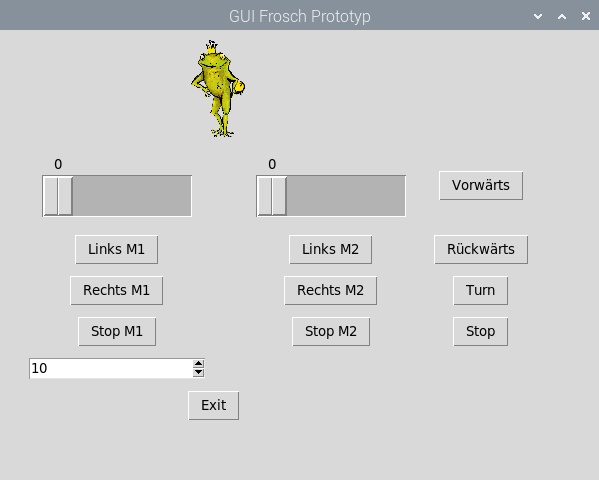
\includegraphics[width=0.6\textwidth]{img/Elektronik/gui_motoren.png}
  \centering
  \caption{GUI Motorensteuerung}
  \label{fig:gui-motoren}
\end{figure}

\newpage

\subsection{Motoren für Fortbewegung}
Für die Fortbewegung wurden 12V DC Getriebemotoren mit Encoder und abgewinkelter Ausgangswelle gewählt \cite{Motoren-Fortbewegung}. Die Motoren werden gleich wie die Motoren der Hubbewegung an eine weitere H-Brücke angeschlossen (Abb. \ref{fig:hbrücke-treppe}).
Um zu Beginn mit dem Roboter für erste Tests vorwärts und rückwärts fahren zu können wurde im zuvor erstellten GUI jeweils ein Button für vor-/rückwärts hinzugefügt.

\begin{figure}[H]
  \includegraphics[width=0.6\textwidth]{img/Elektronik/h_brücke_motoren_fortbewegung.png}
  \centering
  \caption{Anschluss der Motoren an die H-Brücke für Fortbewegung}
  \label{fig:hbrücke-fortbeweg}
\end{figure}

\subsubsection{Encoder}
Encoder oder auch Winkelmesser sind in der Lage, den vorangeschrittenen Winkel bei einer Drehung des Motors zu bestimmen. Mit dieser Winkelangabe und dem Umfang des Rades kann somit die theoretisch gefahrene Distanz bestimmt werden. Die Gefahr dabei ist, dass ein Durchdrehen des Rades in der Software fälschlicherweise als zurückgelegte Distanz aufgenommen werden kann, weshalb der Encoder nicht alleine für die Orientierung verwendet wird sondern von der Kamera unterstützt wird.

\begin{figure}[h]
  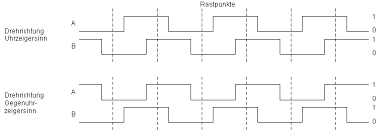
\includegraphics[width=0.7\textwidth]{img/Elektronik/quadrature.png}
  \centering
  \caption{Encoder Signal Kanal A und B}
  \label{fig:encoder-sig}
\end{figure}

Der Encoder gibt bei einer Umdrehung des Motors Rechteckpulse zurück. Durch das Zählen der Pulse in Kanal A und B in einem fixen Zeitintervall und der Anzahl der Pulse pro Umdrehung kann die Geschwindigkeit in rpm wie folgt berechnet werden:

\begin{align}
    Geschwindigkeit\ [rpm] = \frac{\frac{Encoder\ Ticks}{Ticks\ pro\ Umdrehung} \cdot 60\ s}{Zeitintervall\ [s]}
\end{align}

Der Weg kann mittels Umfang des Rades ermittelt werden und in Anzahl Encoder Pulse umgerechnet werden.

\begin{align}
    Anzahl\ Ticks = \frac{Distanz\ [cm]}{Umfang\ Rad\ [cm]} \cdot Ticks\ pro\ Umdrehung
\end{align}

Für beispielsweise eine 90\textdegree-Drehung kann ein Rad vorwärts und das andere Rad rückwärts angesteuert werden, bis die benötigte Distanz erreicht wurde. 


\subsection{Ultraschallsensor}

Ultraschallsensoren sind gut, um ein breites Feld nach Gegenständen abzusuchen. Die Ungenauigkeit von +-5mm, welche in Tests nachgewiesen werden konnte ist dabei vernachlässigbar, da diese Sensoren in erster Linie zur Unterstützung und besseren Einschätzung der Lage dienen.
Im Roboter wird ein solcher Sensoren in Fartrichtung nach vorne verbaut. Der Sensoren wird verwendet, um die Kamera bei der Orientierung und vorallem dem Ausweichen von Hindernissen beim traversieren der Treppe zu unterstützen.

\subsection{Akku}
Im \acrshort{pren1} wurde bereits eine Theoretische Berechnung für die Auslegung des Akkus gemacht. Um eine höhere Genauigkeit für die Kapazität zu erzielen, werden die elektronischen Komponenten wie z.B. die Motoren angesteuert und der Stromverbrauch mittels Multimeter gemessen:
\begin{itemize}
    \item Hauptmotor Hubbewegung: 0.65 A
    \item Hilfsmotor Hubbewegung: 0.35 A
    \item Motoren Fortbewegung: 2 * 0.25 A
    \item Jetson Nano: 0.9 A
\end{itemize}
Daraus folgt 
\[C = {I*t} = \frac{2.4\ A* 12\ min}{60} * 1000 = 480\ mAh\]
Mit Faktor 4 als Reserve ergibt sich ein Modellbauakku mit ca. 2300 mAh von Tattu \cite{Akku-Modellbau}.

Ergänzend zu Erwähnen ist, dass diese Berechnung vor dem Entfernen des zweiten Hubbewegungsmotors gemacht wurde, wodurch die Kapazität des Akkus noch weiter reicht.

\subsection{Schema}

Todo

\newpage

\section{Standsicherheit beim Erklimmen einer Stufe}

Beim Erklimmen einer Stufe ist der kritische Fall, wenn sich die Ausleger horizontal auf einer Linie mit dem Grundkörper befinden. Wenn der Grundkörper auf die nächste Stufe gehoben wird befindet sich die Drehachse der Ausleger am Grundkörper über der Kante der Stufe (siehe Abbildung \ref{fig:Erklimmen}).

\begin{figure}[h]
  \includegraphics[width=1\textwidth]{img/Gerät Aufbau/Standsicherheit.png}
  \centering
  \caption{Gerät beim Erklimmen einer Stufe}
  \label{fig:Erklimmen}
\end{figure}

Um die Standsicherheit in diesem Fall berechnen zu können, wurde das Gewicht des Grundkörpers und der verbundenen Ausleger einzeln gewogen und der Schwerpunkt ermittelt.\\

Gewicht Grundkörper: $m_{GK}$ = 2.63 kg

Gewicht Ausleger: $m_{A}$ = 0.436 kg\\

Abstand Schwerpunkt Grundkörper zur Drehachse: b = 52 mm

Abstand Schwerpunkt Ausleger zur Drehachse: a = 190 mm

\newpage

\begin{align*}
M_{Kipp} = m_{A} * g * a = 0.436 kg * 9.81 m/s^2 * 190 mm = 0.81 Nm
\end{align*}

\begin{align*}
M_{Stand} = m_{GK} * g * a = 2.63 kg * 9.81 m/s^2 * 52 mm = 1.34 Nm
\end{align*}\\

Daraus folgt: $M_{Stand}$ > $M_{Kipp}$

\begin{align*}
Standsicherheit = M_{Stand} / M_{Kipp} = 1.34 Nm / 0.81 Nm = \underline{\underline{1.65}}
\end{align*}







\newpage

\section{Dokumentation Testing}

\subsection{Manuelles Testing}
Für aller erste Tests der Motorenansteuerung, wurde das GUI zur Hilfe genommen, welches in Pren1 entwickelt wurde. Kurz daraufhin sollten die ersten Softwarekomponenten (\texttt{LiftingController}, \texttt{AlignmentChecker}, \texttt{CruisingController}) getestet werden. Dies wurde in einem ersten Durchlauf mithilfe des interaktiven Python Modus in der Konsole erreicht. Daraufhin wurde jedoch eine Fernbedienung geschrieben. Mehr dazu im Abschnitt \ref{}.

\subsubsection{Hubbewegung}

\subsubsection{Ablauf}

Um den ersten Sprint erfolgreich abzuschliessen, wurden alle Teile, welche bereits im Pren1 konstruiert wurden, mit den 3D-Druckern im Team produziert. Die Elektromotoren, welche für die Hubbewegung zuständig sind wurden verbaut, ebenso wie die Motoren für die Fortbewegung um das Gewicht realistischer zu simulieren. Somit konnte die Hubbewegungen getestet werden und das 3D-Konstrukt auf Schwachstellen untersucht werden.

\begin{figure}[H]
  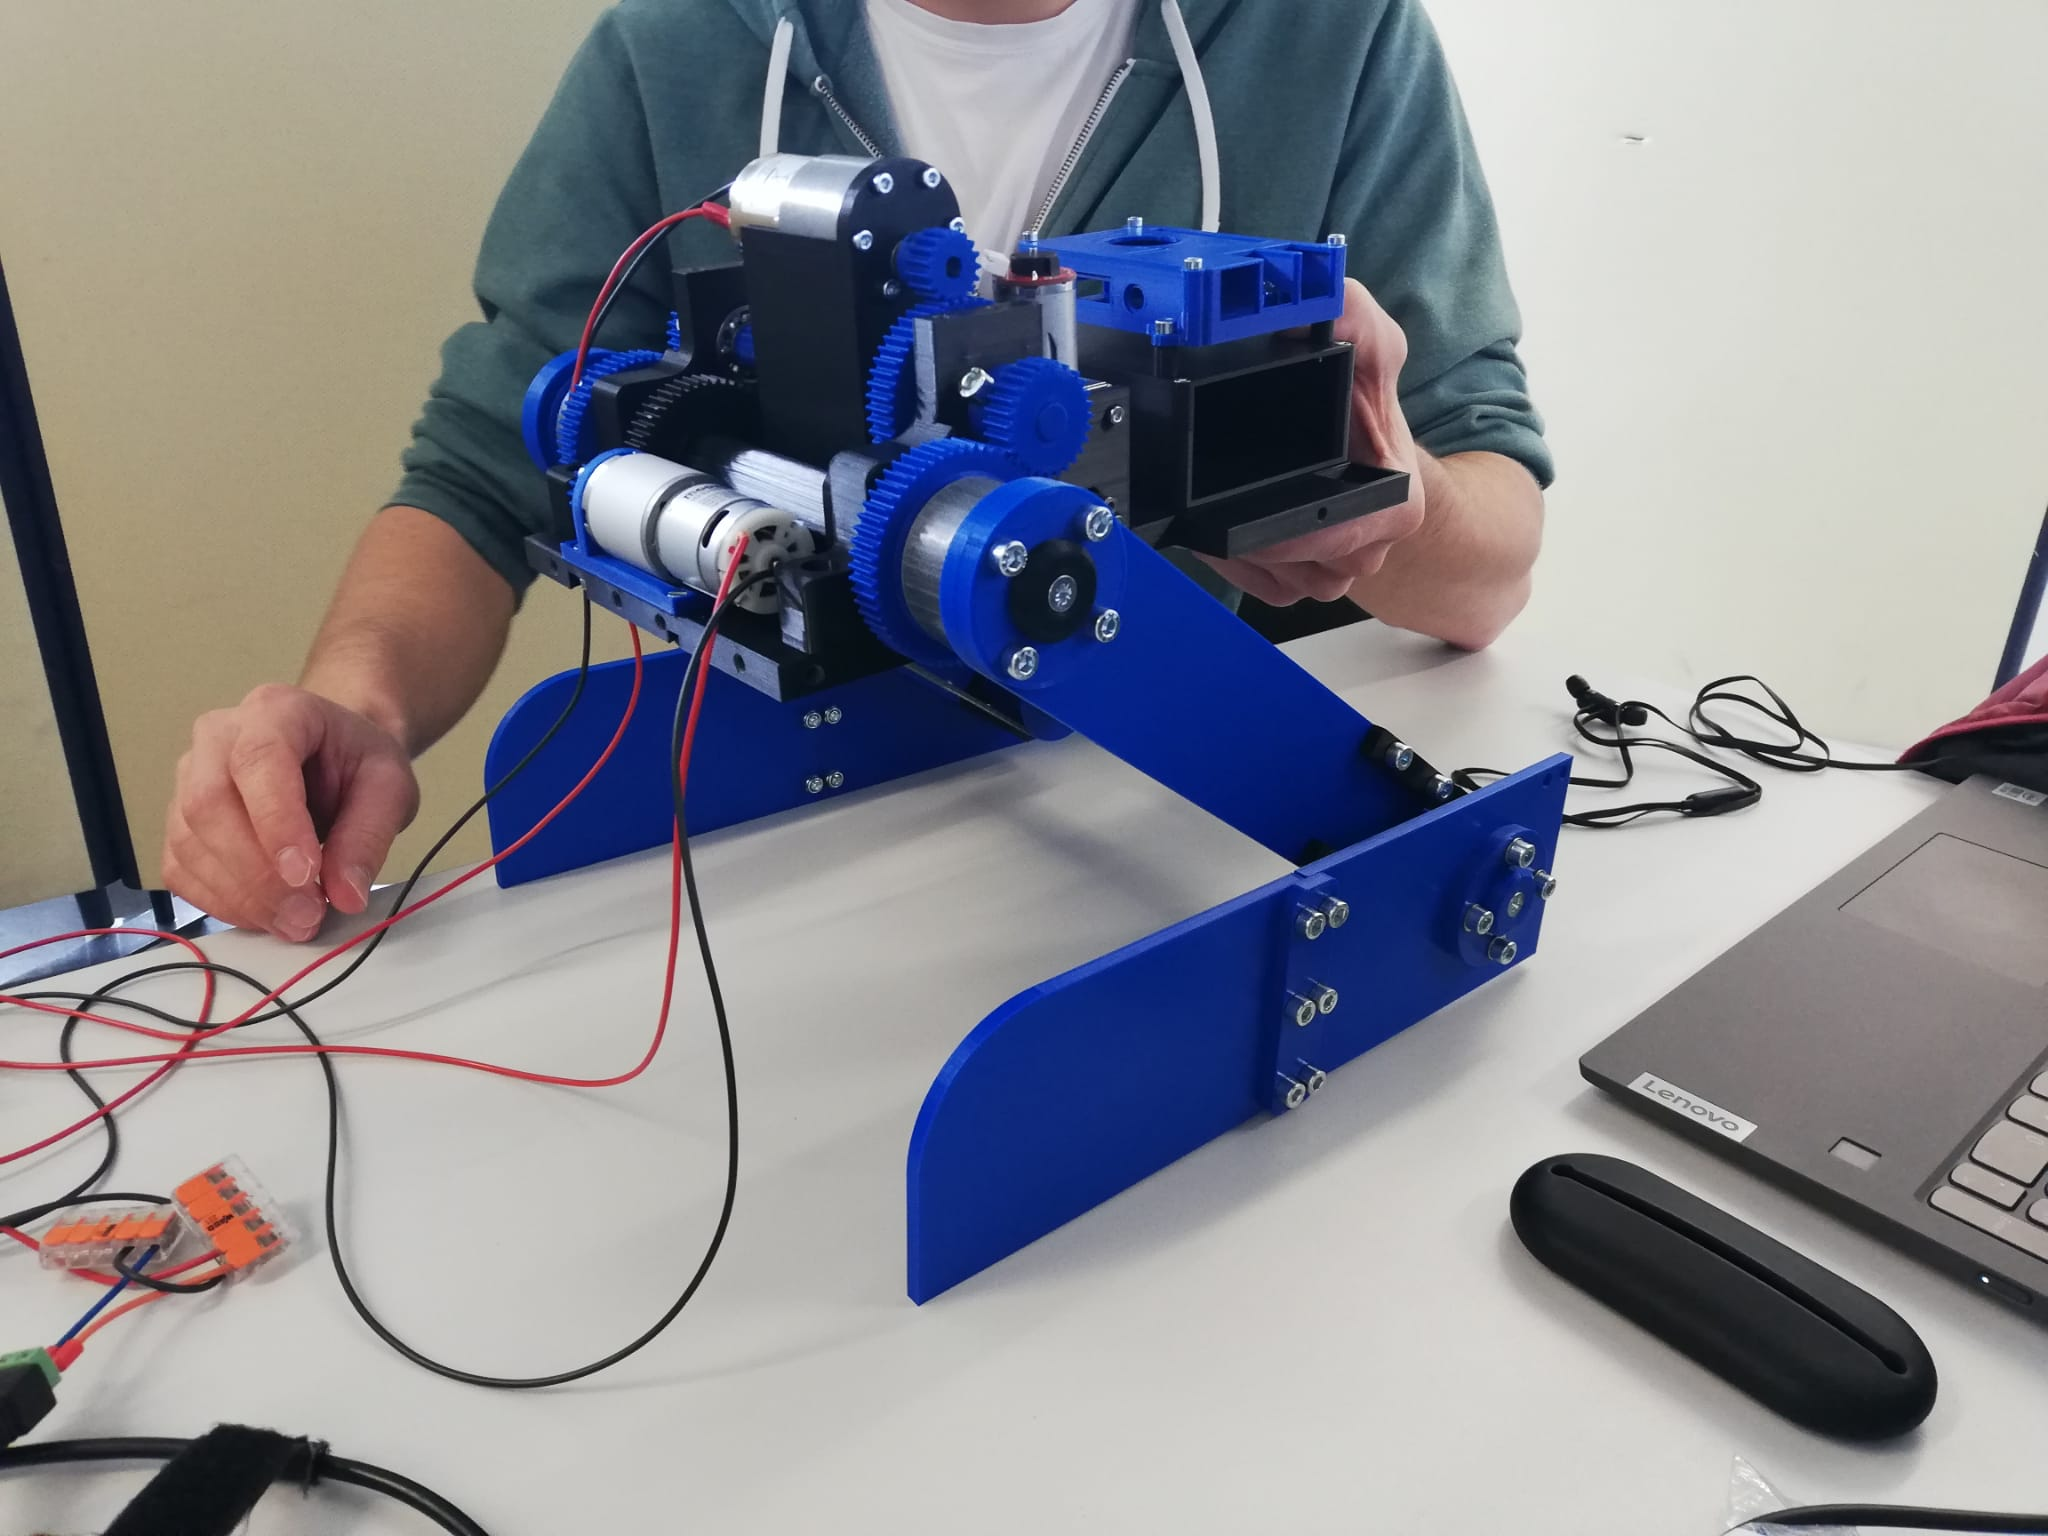
\includegraphics[width=0.65\textwidth]{img/Sprint1/pren1_sprint1_1.png}
  \centering
  \caption{Sprint 1 - Erste Prototypentests}
  \label{fig:sprint-backlog-1}
\end{figure}
In diesem Test offenbarten sich einige Schwachstellen. So konnte ein Zahnrad nicht genügend Druck auf die Motorenwelle halten, was zu einem Durchdrehen des Motors geführt hat.
Die Schwachstellen des ersten Prototypen konnten schnell neu gedruckt werden, was zu einem schnellen zweiten Versuch führte.

\begin{figure}[H]
  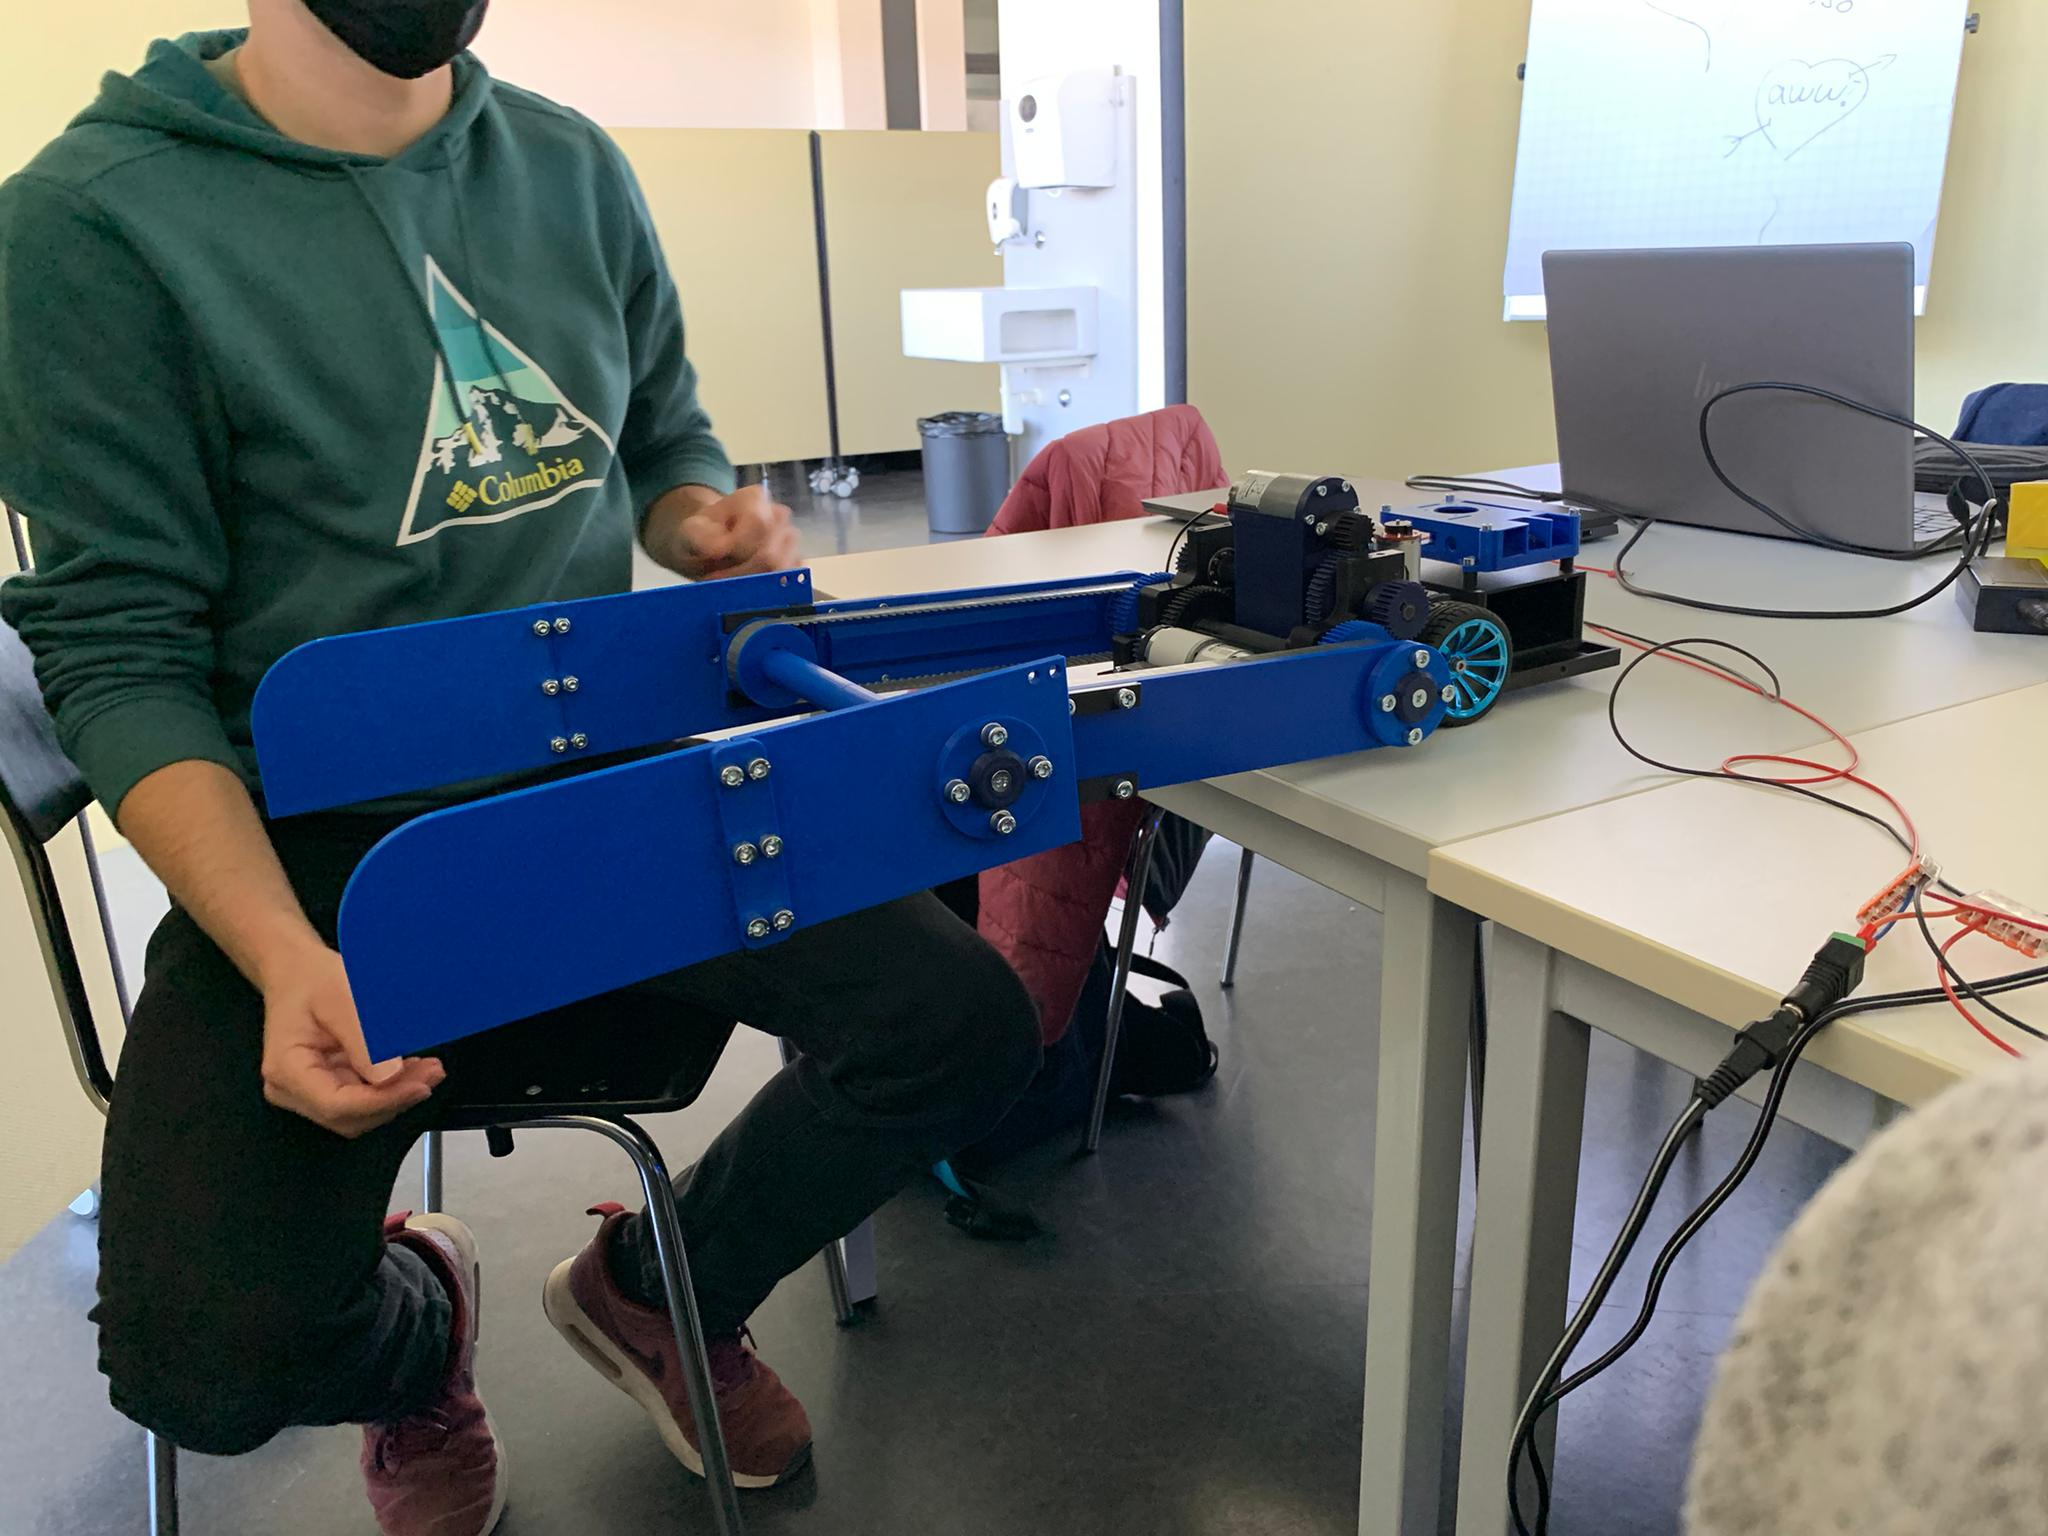
\includegraphics[width=0.65\textwidth]{img/Sprint1/pren1_sprint1_2.png}
  \centering
  \caption{Sprint 1 - Zweite Tests}
  \label{fig:sprint-backlog-1}
\end{figure}
Mit den neuen Teilen war es möglich, die erste wie auch die zweite Hubbewegung ohne Überbelastung einzelner Teile durchzuführen.
Die volle Drehbarkeit der Ausleger wird nur noch von den Stromkabeln an den Motoren eingeschränkt. In diesem zweiten Test wurden wiederum neu angekommene Teile direkt verbaut um langsam an das Zielgewicht heranzukommen.

Mit diesem Roboter konnten auch die ersten Versuche auf einer Treppe durchgeführt werden. Dazu wurde der Roboter in verschiedenen Positionen auf der Treppe platziert und die erste Hubbewegung ausgeführt.

\begin{figure}[H]
  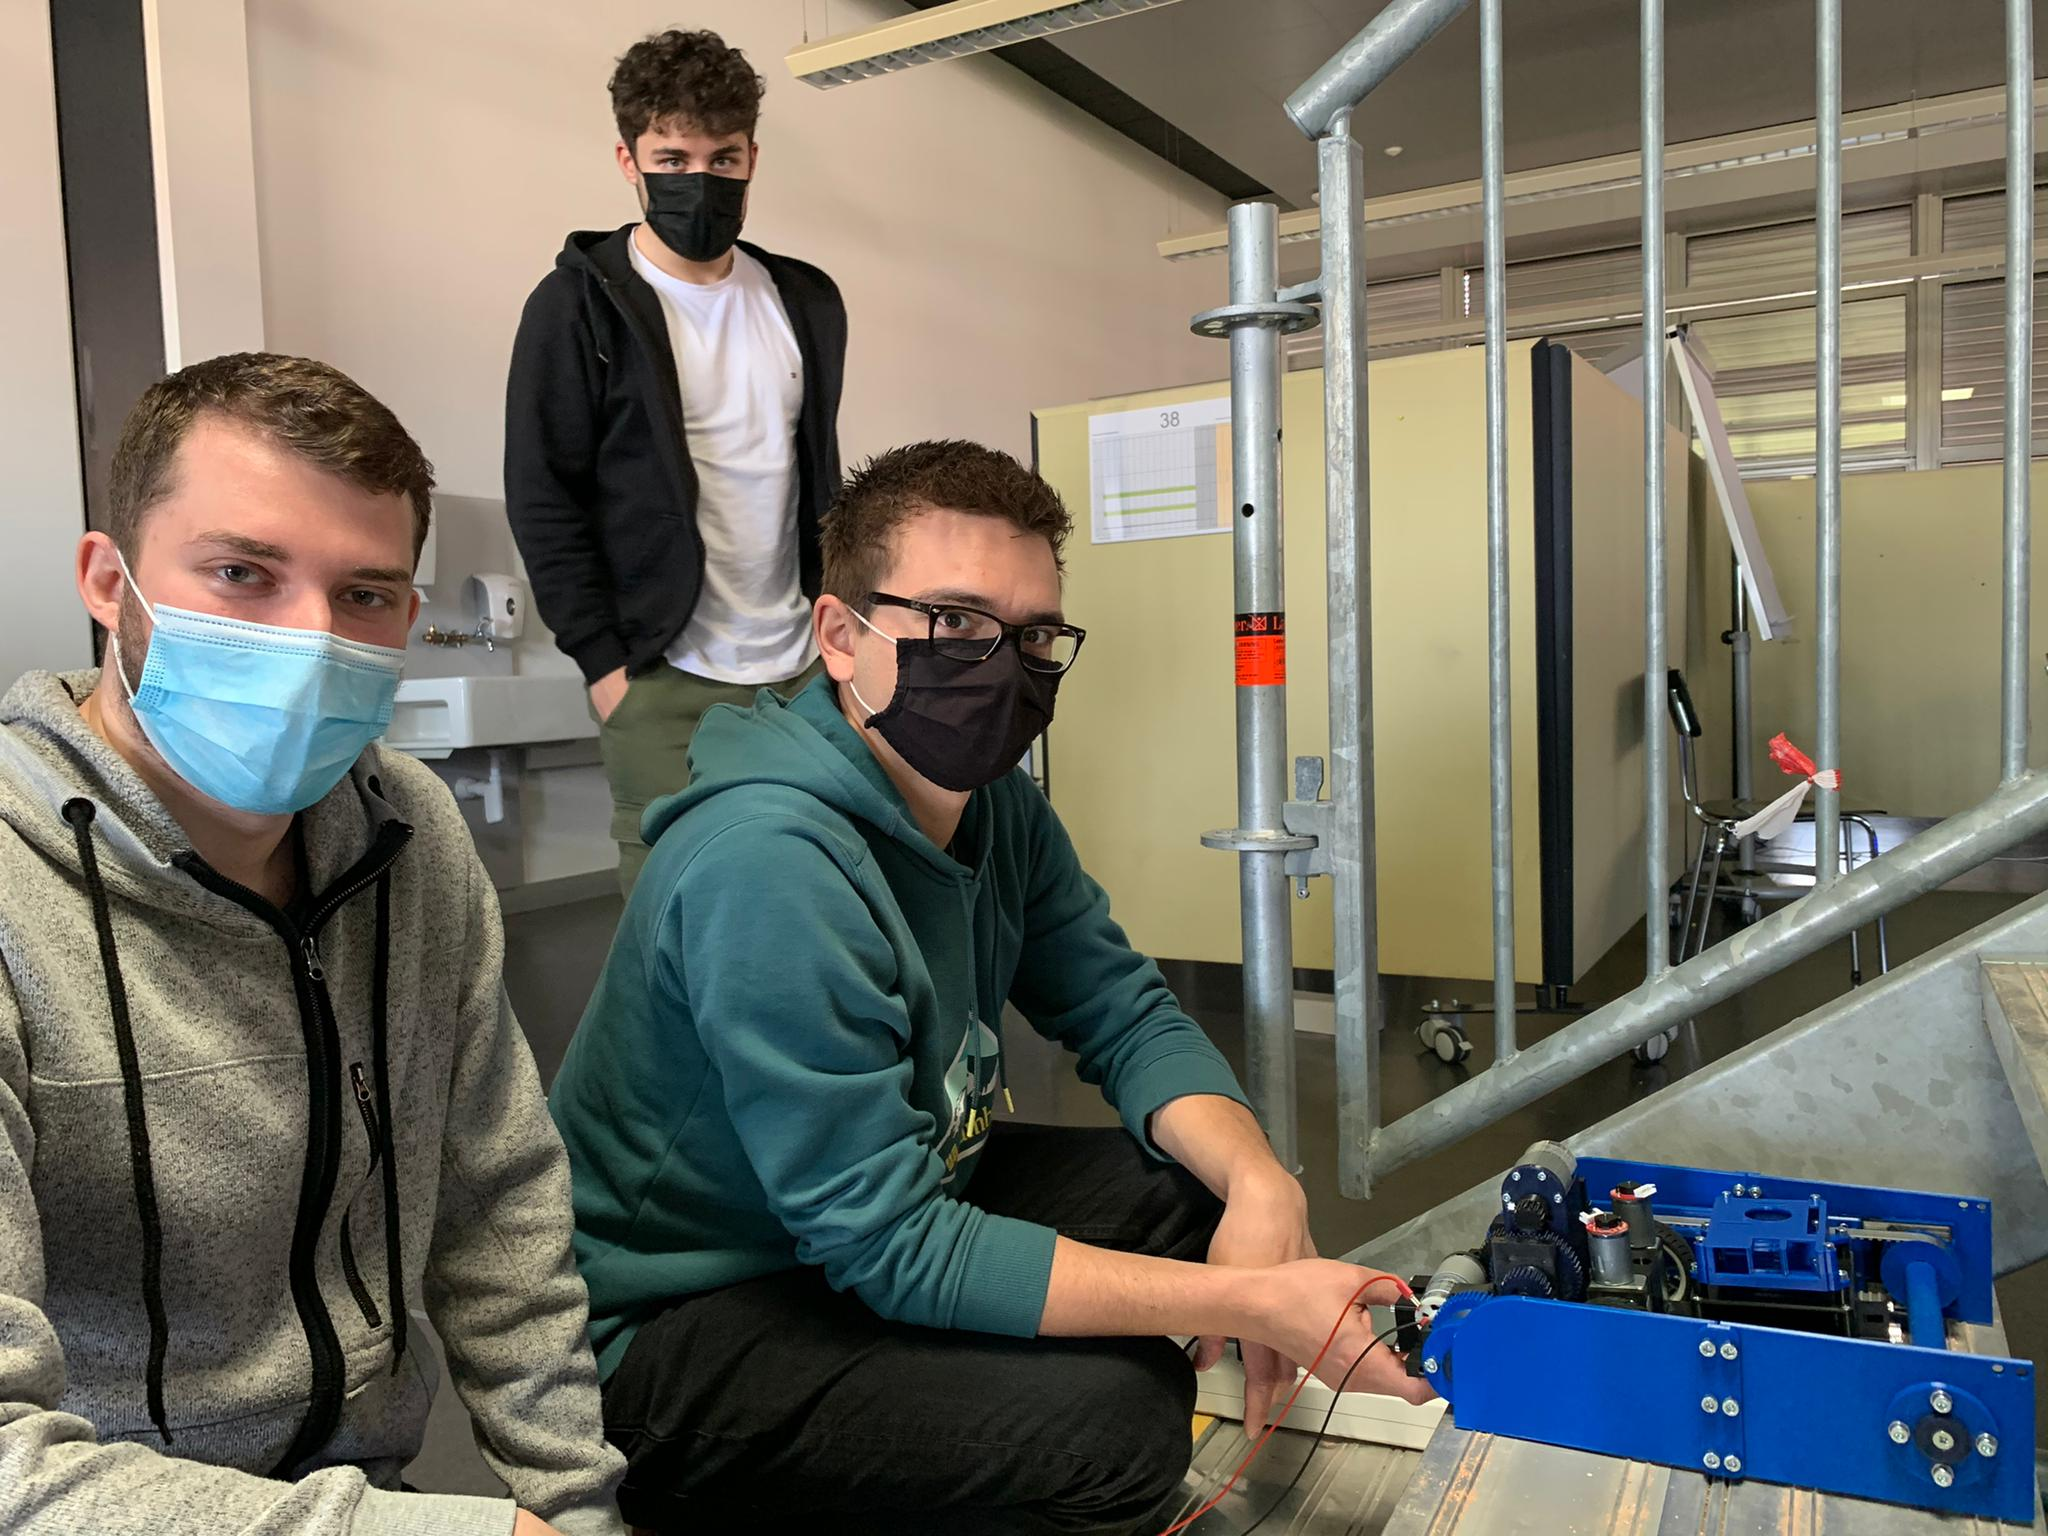
\includegraphics[width=0.65\textwidth]{img/Sprint1/pren1_sprint1_3.png}
  \centering
  \caption{Sprint 1 - Erste Treppentest}
  \label{fig:sprint-backlog-1}
\end{figure}

In diesem Test konnte einiges über die Form der Ausleger und dessen Optimierungspotential gelernt werden. Diese Verbesserungen werden im nächsten Prototypen angewendet.

Ein weiterer Punkt für Optimierungen sind die beiden Achsen des Huberts. Das Grundgerüst aus 3D-Druck erfüllt seinen Zweck vollumfänglich. Die Achsen selbst welche momentan noch gedruckt sind werden durch Aluminium-Achsen getauscht. Dies auf der einen Seite aufgrund der Reibung von Plastik auf Plastik welche unnötig Energie verbraucht und andererseits weil die Achsen für die Struktur von entscheidender Bedeutung sind. 

\subsubsection{Ergebnisse}

Der erste Sprint und somit die ersten Prototypentests haben Schwachstellen und Potential enthüllt. Der Plan, welcher im Pren1 erarbeitet wurde, ist umsetzbar. Es benötigt noch einiger Optimierungen um das volle Potential auszuschöpfen, das wird fortlaufend neben dem Implementieren neuer Funktionen geschehen.

\subsubsection{Fortbewegung}

Die Fortbewegung soll möglichst auf engem Raum stattffinden können. Deshalb werden in diesem Bereich zwei mögliche Drehmethoden getestet. Die einfachere der beiden ist das vor-, oder rückwärtsdrehen eines einzelnen Rades. Die etwas aufwändigere ist das vor- bzw rückwärts drehen eines Rades während das andere Rad in die entgegengesetzte Richtung dreht.

Nach diesem Test hat sich ergeben, dass die zweite Variante mit dem ansteuern beider Motoren in unterschiedliche Richtungen eine Drehung nahezu auf einer Stelle gewährleistet. Somit wird in der Software diese Art der Drehung implementiert.

\subsection{Testing mit Software}
Um die einzelnen Verhalten des Roboters, wie z.B. Hubbewegung, Ausrichtung zur Treppe, Fortbewegung, 90\textdegree-Drehungen effizient testen zu können, wurde eine Fernbedienung über SSH entwickelt. Mithilfe dieser Fernbedienung ist es dem Team möglich, den Roboter über die Tastatur des Notebooks zu steuern. Mit dem Notebook muss man sich lediglich per SSH auf das Controllerboard mit dem embedded Linux verbinden und das Python-Modul \texttt{remote\_control\_ssh.py} starten. Hierbei war die Schwierigkeit, dass Keyboard Inputs über SSH nicht direkt eingelesen werden können, wie das bei einer Tastatur welche direkt mit dem Controllerboard verbunden ist, der Fall ist. Dies aus dem Grund, dass Keyboardinputs nicht standardmässig über SSH übertragen werden. 

Dieses Problem konnte umgangen werden, indem man auf dem Notebook ein X-Server \cite{Wikipedia-X-Window-System} startet und die SSH Verbindung mit einem X11-Forwarding startet. Das \texttt{remote\_control\_ssh.py} Modul startet dann ein Window auf dem X-Server welcher auf dem Notebook gestartet wurde. Die Keyboard Inputs werden dann über die X-Session an das Controllerboard übertragen. 

Als X-Server wurde der Xming X Server fpr Windows verwendet \cite{Xming-X-Window-Server-Download}.

Das X11-Forwarding bei der SSH Verbindung kann im Putty unter Connection/ssh/x11 enabled werden. 

\begin{figure}[H]
  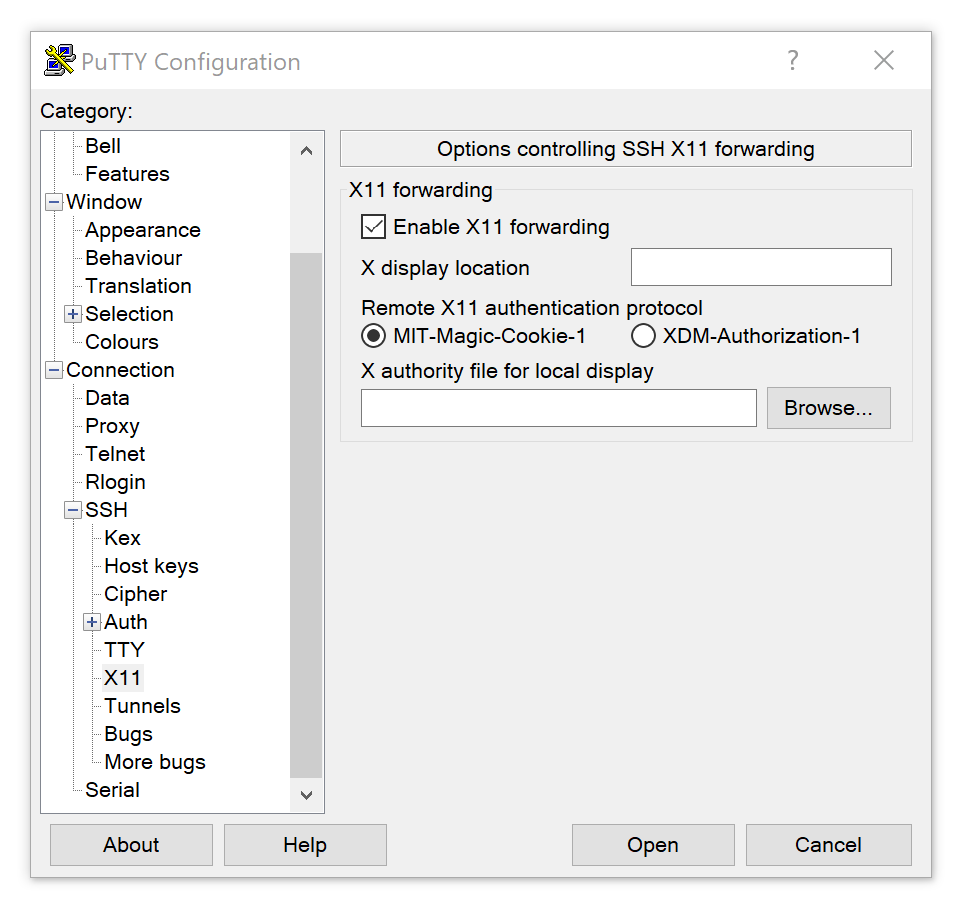
\includegraphics[width=0.65\textwidth]{img/remote_control/putty_x11.PNG}
  \centering
  \caption{Putty X11-Forwarding}
  \label{fig:putty_x11_forwarding}
\end{figure}

Bie einer SSH Verbindung aus der Konsole fügt man lediglich den Parameter -X (gross X) hinzu. Der Befehl könnte dann folgendermassen aussehen: \texttt{ssh -X raspi\_hslu}.

Die Bedienung wurde folgendermassen festgelegt:
\begin{center}
\begin{table}[H]
\begin{tabular}{|l|r|r|r|r|}
\hline
\textbf{Kommando} & \textbf{Tastaturbelegung} &
\textbf{Keycode}\\
\hline
Forward & W & 119\\
\hline
Backward & S & 115\\
\hline
Turn left & A & 97\\
\hline
Turn right & D & 100\\
\hline
Stop cruise & Q & 113\\
\hline
Main Motor Forward & E & 101\\ 
\hline
Main Motor Backward & R & 114\\ 
\hline
Main Stop & X & 120\\ 
\hline
Turn right 90 & F & 102\\ 
\hline
Turn left 90 & G & 101\\ 
\hline
Approach stair & 1 & 49\\ 
\hline
Align & 2 & 50\\ 
\hline
Climb step & 3 & 51\\ 
\hline
Tof distance & 4 & 52\\ 
\hline
Straight forward 50cm & c & 99\\ 
\hline
Emergency stop & [space] & 32\\ 
\hline
Quit & [esc] & 27\\ 
\hline
\end{tabular}
\caption[Tastaturbelegung für die Fernsteuerung]{Tastaturbelegung für die Fernsteuerung}
\label{tab:entwicklungsaufwand}
\end{table}
\end{center}


\subsection{Fortbewegung}

Die Fähigkeit, geradeaus zu fahren ist unter anderem für das Traversieren auf der Treppe von grosser Bedeutung, weshalb die Winkelmotoren der Fortbewegung spezifisch mit Encoder gewählt wurden. Mithilfe dieser Encoder können die Motoren so gesteuert werden, dass die Räder immer gleich schnell drehen. Dies wird in einer eigenen Klasse implementiert. Ebenfalls wird ein Modul programmiert, welches nach Eingabe eines Gradwertes eine möglichst genaue Drehung gewährleistet.

\begin{figure}[H]
  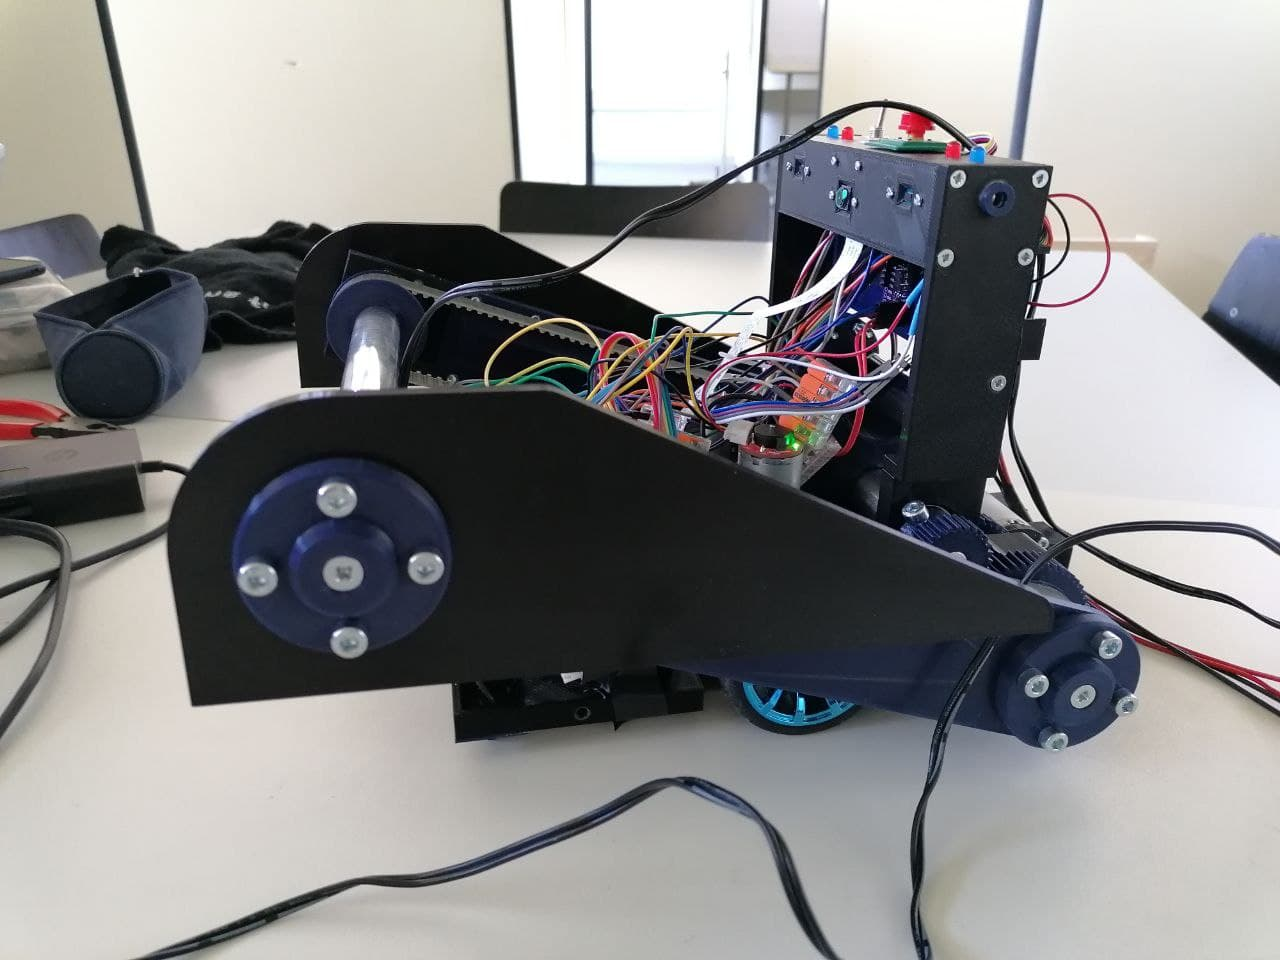
\includegraphics[width=0.65\textwidth]{img/Sprint3/fortbewegung.jpg}
  \centering
  \caption{Fortbewegungstests}
  \label{fig:Fortbewegungstests}
\end{figure}
In diesen Tests konnte festgestellt werden, dass aufgrund von dem geringen Schlupf zwischen dem Motor und den Rädern eine leichte Abweichung nicht umgangen werden kann. Dieser beläuft sich jedoch auf wenige Millimeter auf eine Fahrdistanz von 0.5 Meter. Somit kann ein zuverlässiges Geradeausfahren sichergestellt werden.

Die Drehung um die eigene Achse ist ein Punkt, bei welchem es viele Lösungsmöglichkeiten gibt. Das Ziel ist es, eine Drehung auf möglichst kleinem Raum zu ermöglichen. Dabei können die Räder verschieden schnell angesteuert werden um die Drehung zu optimieren. In den Tests hat sich ergeben, dass die Räder bereits in der Planung sehr gut plaziert wurden, weshalb die Räder gleichmässig angetrieben werden können ohne den Radius signifikant zu vergrössern.



\subsection{Autonome Hubbewegung}

Der nächste Schritt ist die automatisierung der Hubbewegung. Dazu werden weitere Komponente im Grundgerüst verbaut und verkabelt. Dazu gehören neben den Motoren für die Hubbewegung auch die H-Brücken dieser Motoren. Ebenfalls werden bereits die Fortbewegungsmotoren mit der dafür vorgesehehenen H-Brücke verbunden. Weiter werden die Taster und der Schalter ausgemessen und Kabel angelötet um später Zeit einzusparen. Der Akku wird noch nicht verbaut aufgrund einer Lieferverzögerung, weshalb der erste Test auch noch mit einem Kabel zur Stromversorgung verwendet. Gesteuert wird der Roboter in diesem Versuch von einem Raspberry Pi 3B.
Auch wenn das Raspberry nicht der finale Controller des Roboters ist, können somit die in Python geschriebenen Funktionen getestet und verfeinert werden.
Das Ziel dieses Tests ist es, eine automatisierte, über den Controller gesteuerte Hubbewegung.

Dazu werden die ersten Tests auf einem Tisch durchgeführt und der Roboter manuell abgefangen bevor der Erste Treppentest durchgeführt wird

\begin{figure}[H]
  \includegraphics[width=0.65\textwidth]{img/Sprint2/pren2-Löten.jpg}
  \centering
  \caption{Sprint 1 - Zweite Tests}
  \label{fig:sprint-backlog-1}
\end{figure}

Zu Beginn werden alle Komponente des Roboters einzeln über den Controller angesteuert und getestet, wie sich diese verhalten. Dabei fällt auf, dass die menschliche Reaktionszeit der beschränkende Faktor ist beim Erklimmen der Treppe. Eine Hubbewegung ist möglich aber nur sehr langsam. Um die Hubbewegung vollkommen autonom gewährleisten zu können werden die einzelnen Module in Verhalten eingeteilt welche eine Aufgabe erledigen und dazu die Module eigenständig verwendet.



\subsection{Anfahren der Treppe}

Um an die Treppe heranfahren und ausrichten zu können, werden die Module der Fortbewegung in Kombination mit den beiden TOF-Sensoren benötigt, welche auf Höhe der Treppenkante montiert werden. Die Sensoren liefern dabei nicht nur die Werte für die Distanz zur Treppe sondern auch die Ausrichtung zur Treppe. Ist der Abstand zur Treppe wie gewünscht, stoppt der Frosch und dreht sich noch soweit um die eigene Achse, bis der Distanzunterschied beider Sensoren im vorbestimmten Toleranzbereich ist und der Roboter somit für die nächste Hubbewegung bereit ist.
Der Controller startet das Verhalten zum Anfahren und Ausrichten zur Treppe welches wiederum die programmierten Module verwendet. Dieser Aufbau der Software ermöglicht ein sehr flexibles Vorgehen und eine gute Überschaubarkeit des Codes.

\begin{figure}[H]
  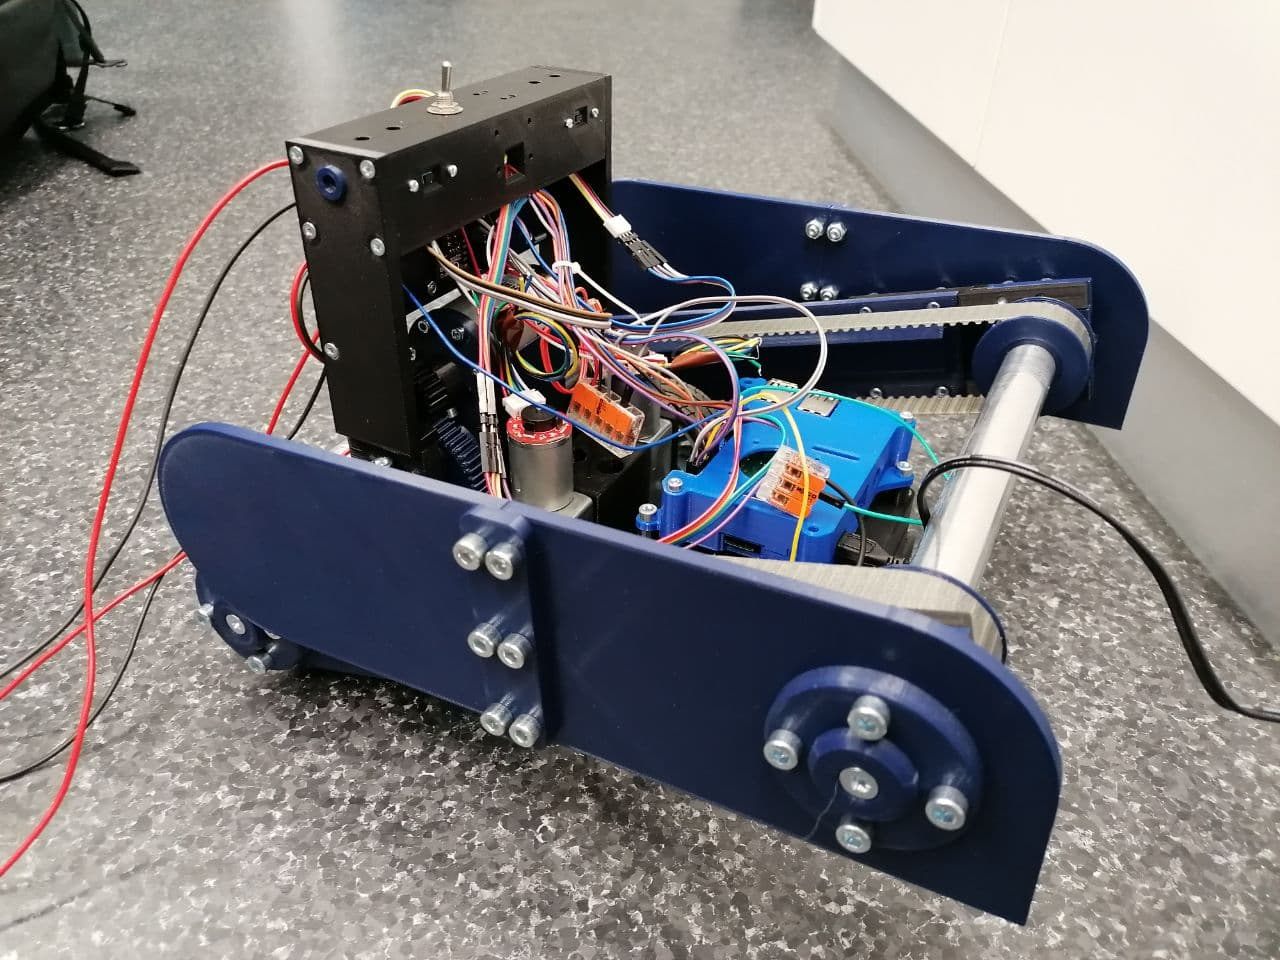
\includegraphics[width=0.65\textwidth]{img/Sprint2/pren2_ausrichten-anfahren.jpg}
  \centering
  \caption{Roboter beim Test zur automatischen Ausrichtung}
  \label{fig:sprint-backlog-1}
  \end{figure}
  
  
\subsection{Bilderkennung}

Um den Pfad zu berechnen müssen die Gegenstände auf der Treppe gefunden werden. Dazu wird eine Datenbank mit möglichst vielen Bildern gesammelt, auf welchen die Ziegelsteine manuell eingezeichnet werden. Unsere Datenbank umfasst ungefähr 420 Bildern und ermöglicht dem Computer somit eine zuverlässige vergleichsbasis um die Hindernisse selbstständig zu finden.

Diese Bilder werden mit einem Mock-Up und einer selber entwickelten App gemacht um einerseits die Kamera auf der richtigen Höhe zu fixieren und andererseits um die Handhabung zu vereinfachen.



\begin{figure}[H]
  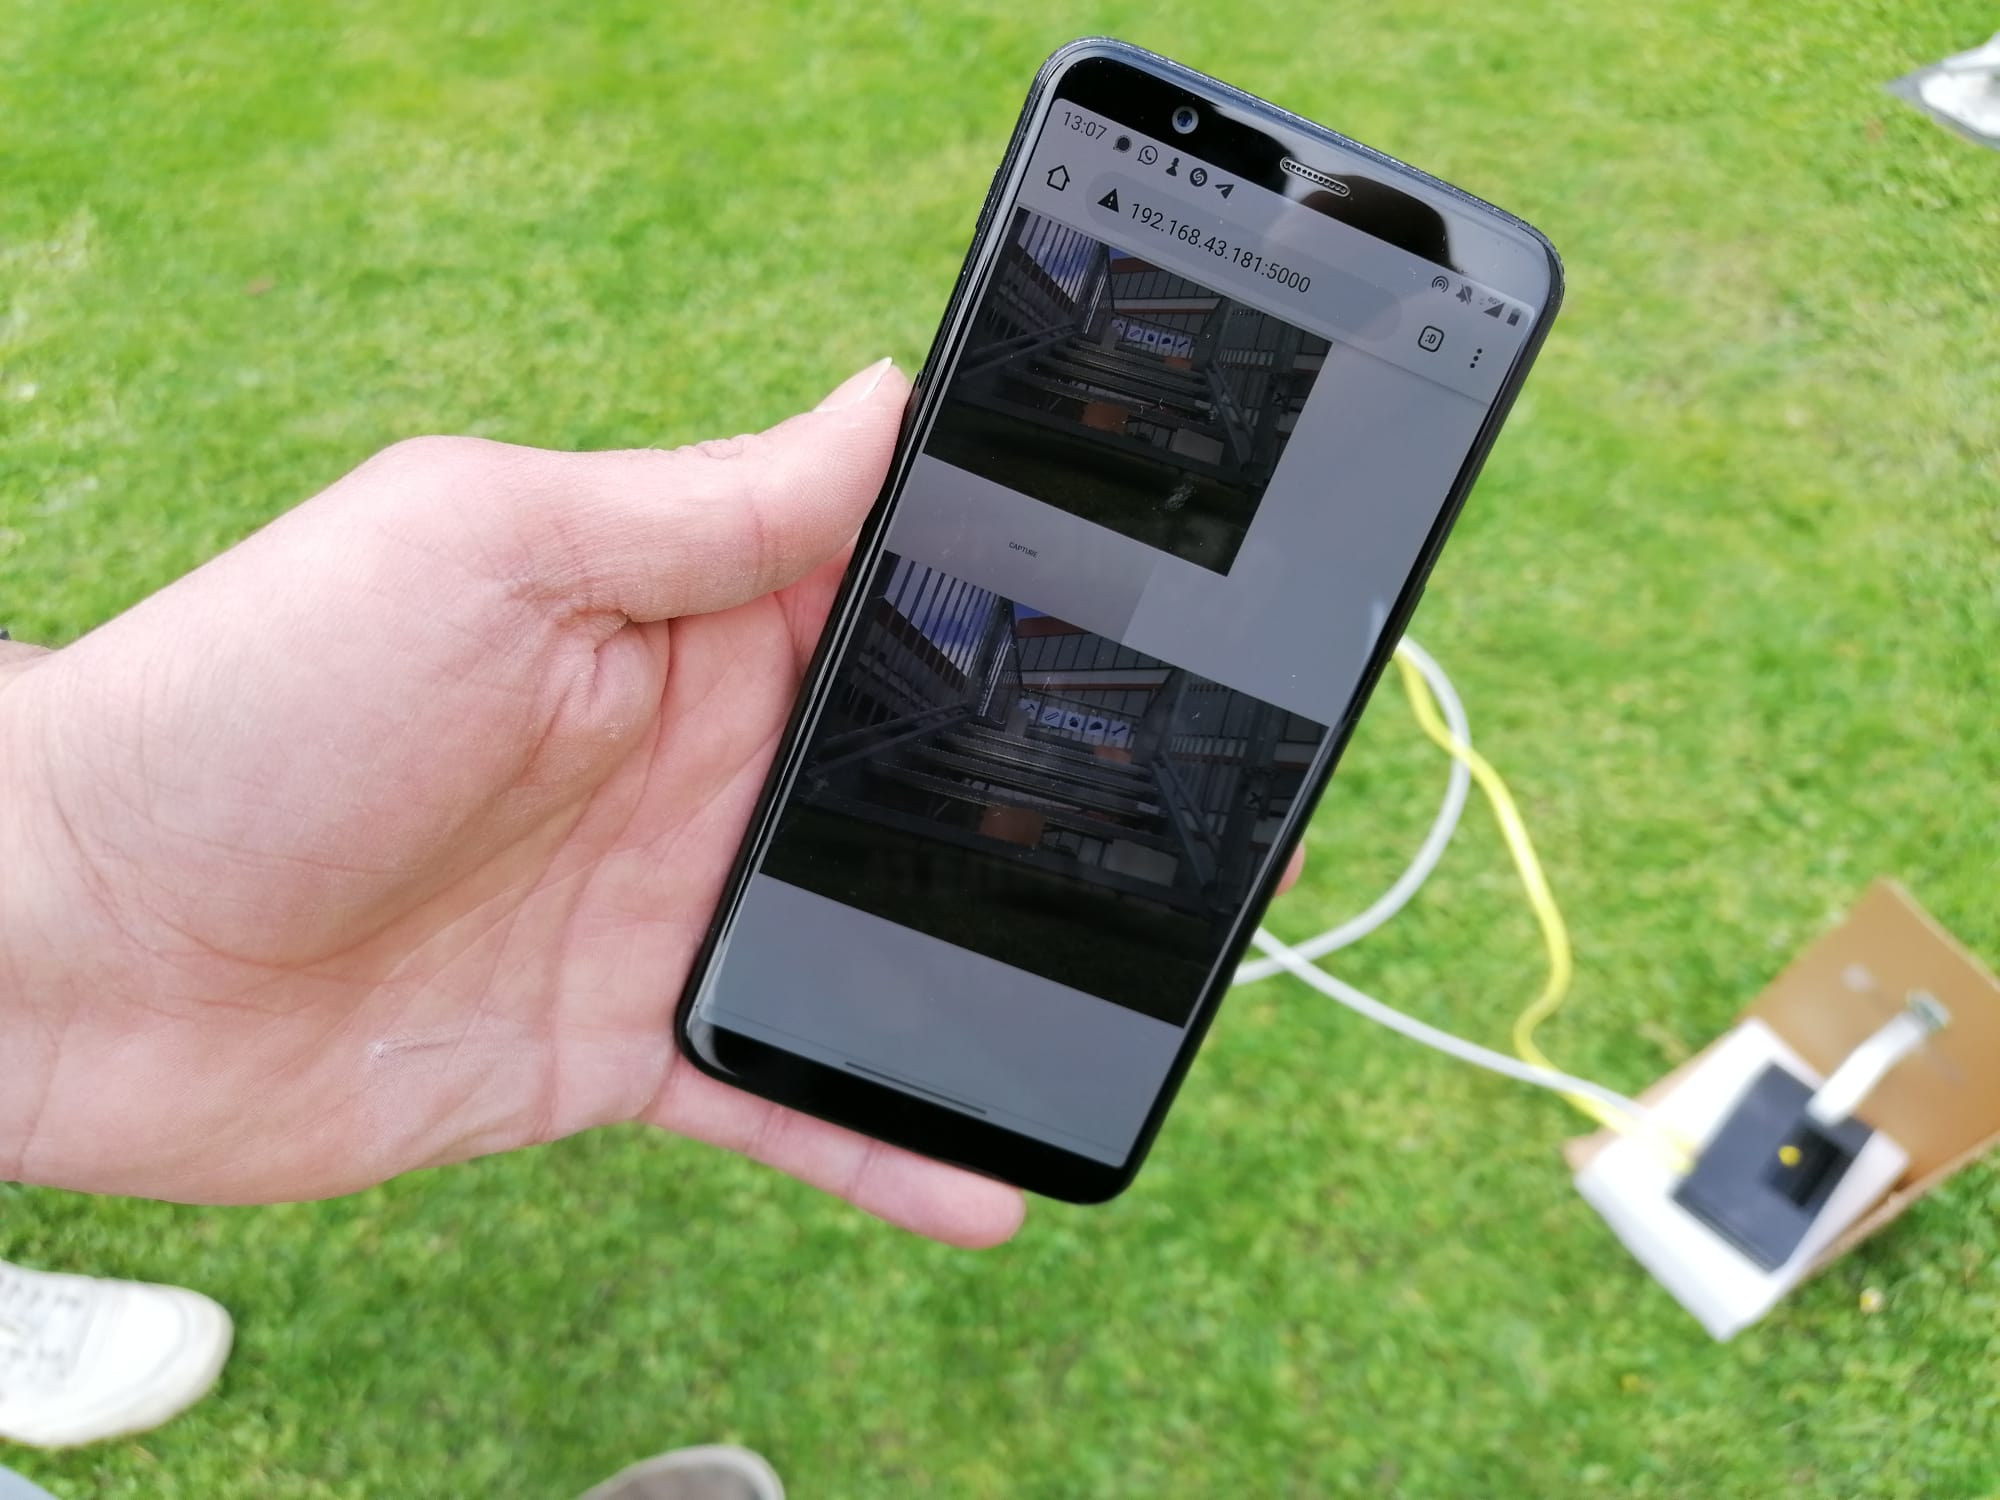
\includegraphics[width=0.65\textwidth]{img/Sprint3/Sprint3_Bildersammlung.jpeg}
  \centering
  \caption{Vorgehen zur Aufnahme der Referenzbilder}
  \label{fig:Aufnahme der Referenzbilder}
  \end{figure}
  
  Zusätzlich werden Bilder gemacht, um die Piktogrammerkennung im Start- und Zielbereich zu machen. Dies wiederum um den bereits erstellten Piktogrammerkennungsalgorithmus zu testen und zu verfeinern.
  
  
  \begin{figure}[H]
  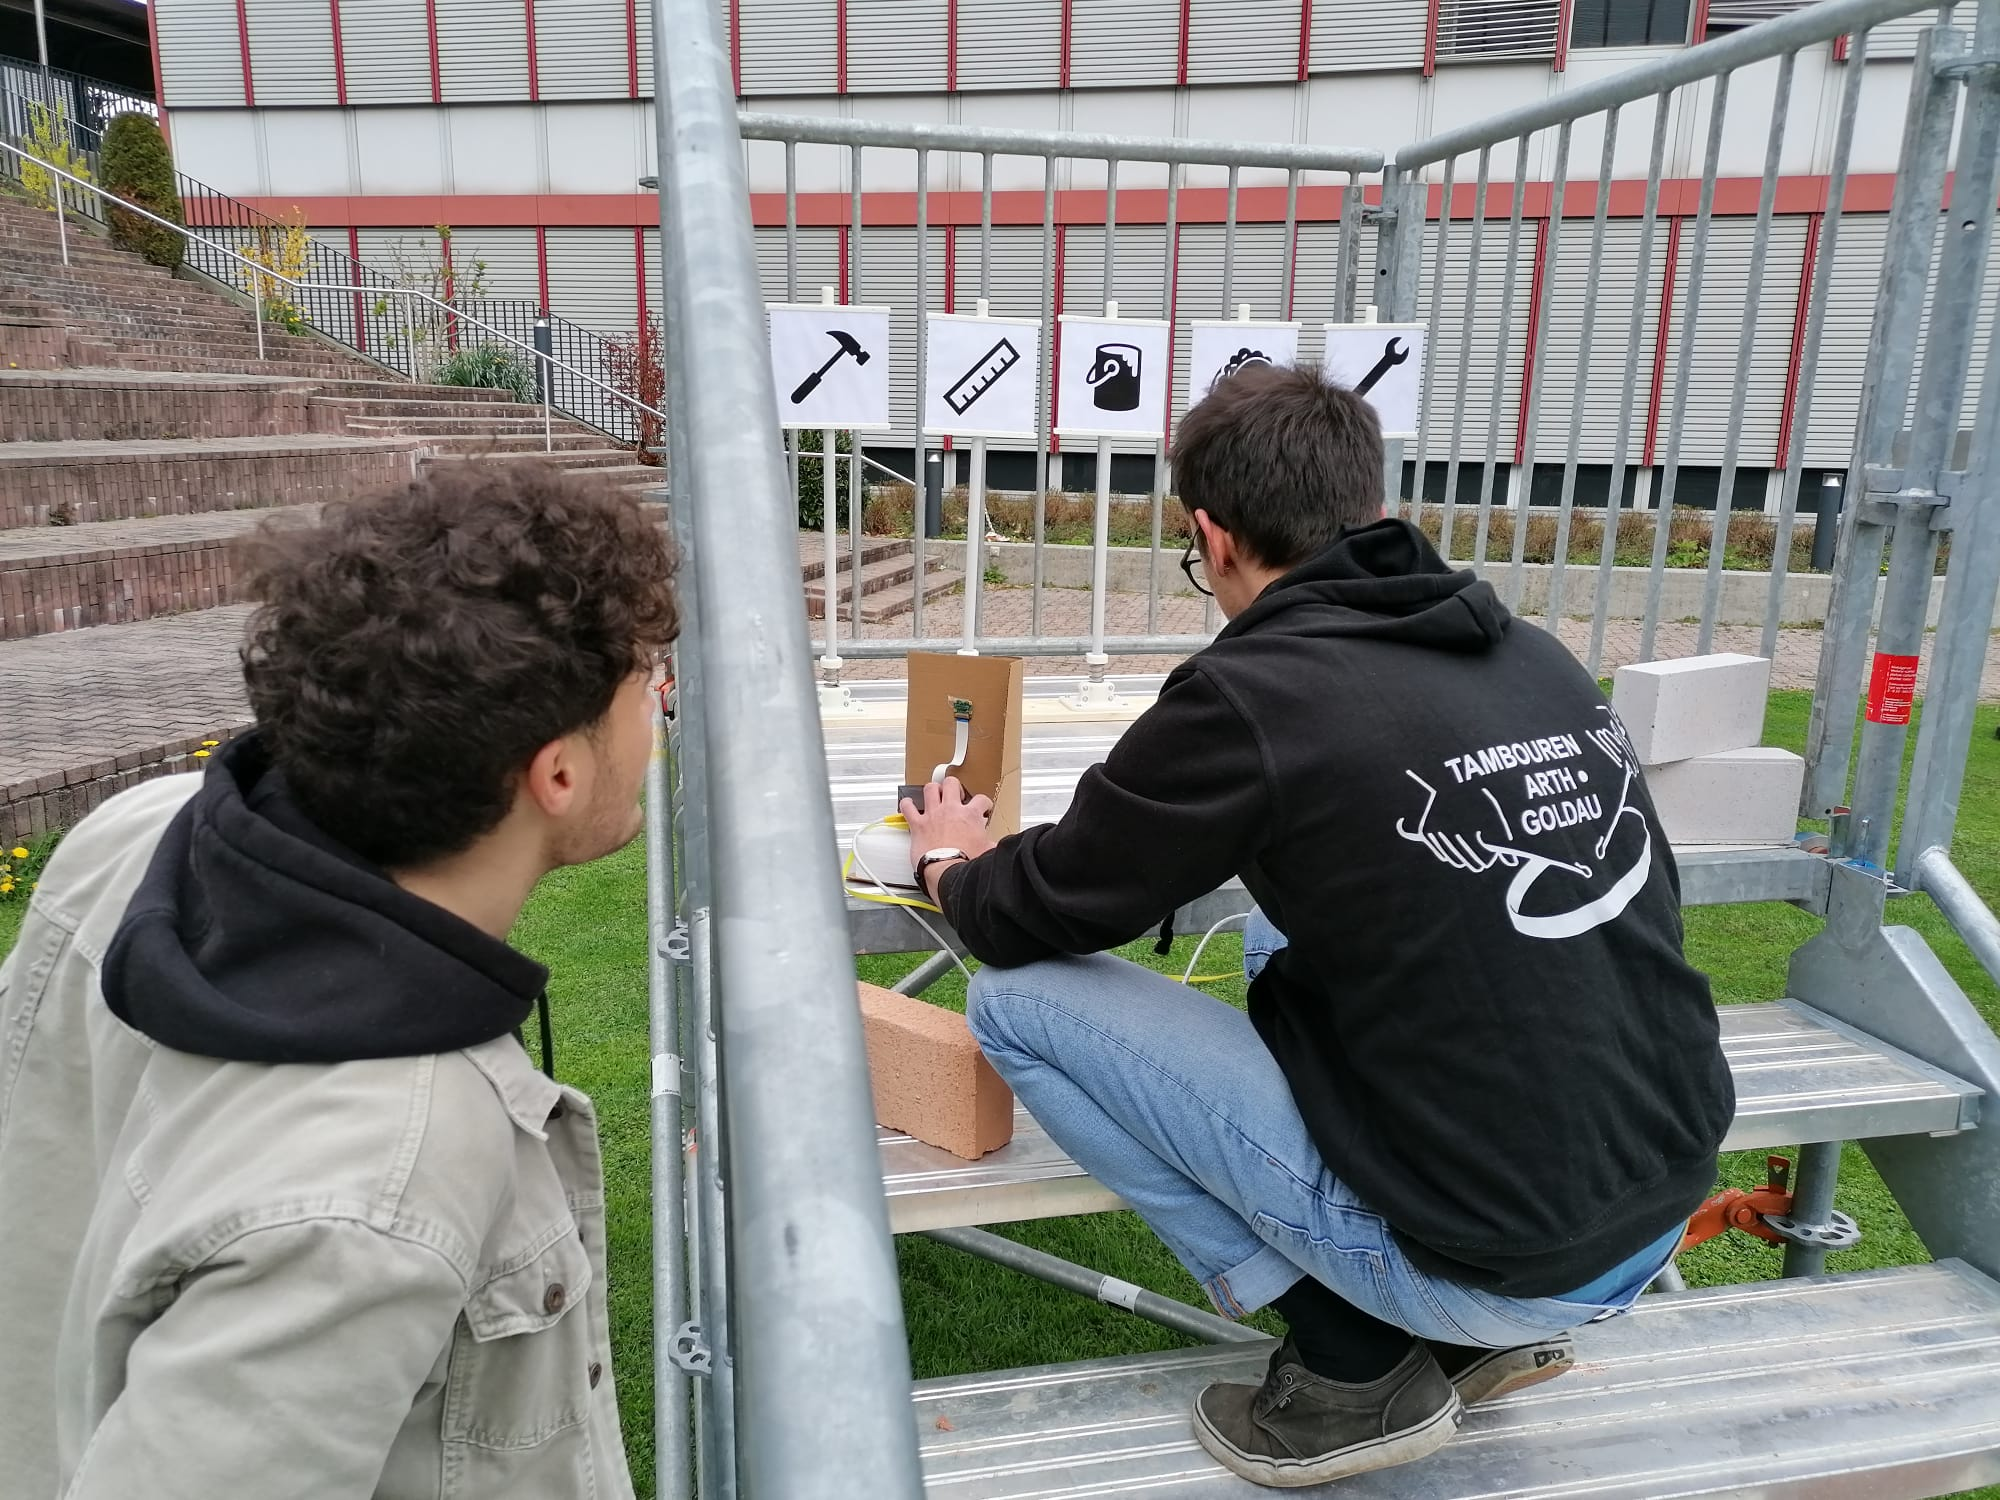
\includegraphics[width=0.65\textwidth]{img/Sprint3/Sprint3_Bildersammlung2.jpeg}
  \centering
  \caption{Das Team bei der Aufnahme der Referenzbilder}
  \label{fig:Aufnahmeprozess der Referenzbilder}
  \end{figure}
  
  
\subsection{Funktionsweise mit Akku}\label{sec:Funktionsweisemit Akku}

Um ein autonomes Fahren gewährleisten zu können, muss der Roboter mit einem Akku betrieben werden können. Dazu werden verschiedene Schritte benötigt. So wird erstmals das Jetson Nano verwendet.

 \begin{figure}[H]
  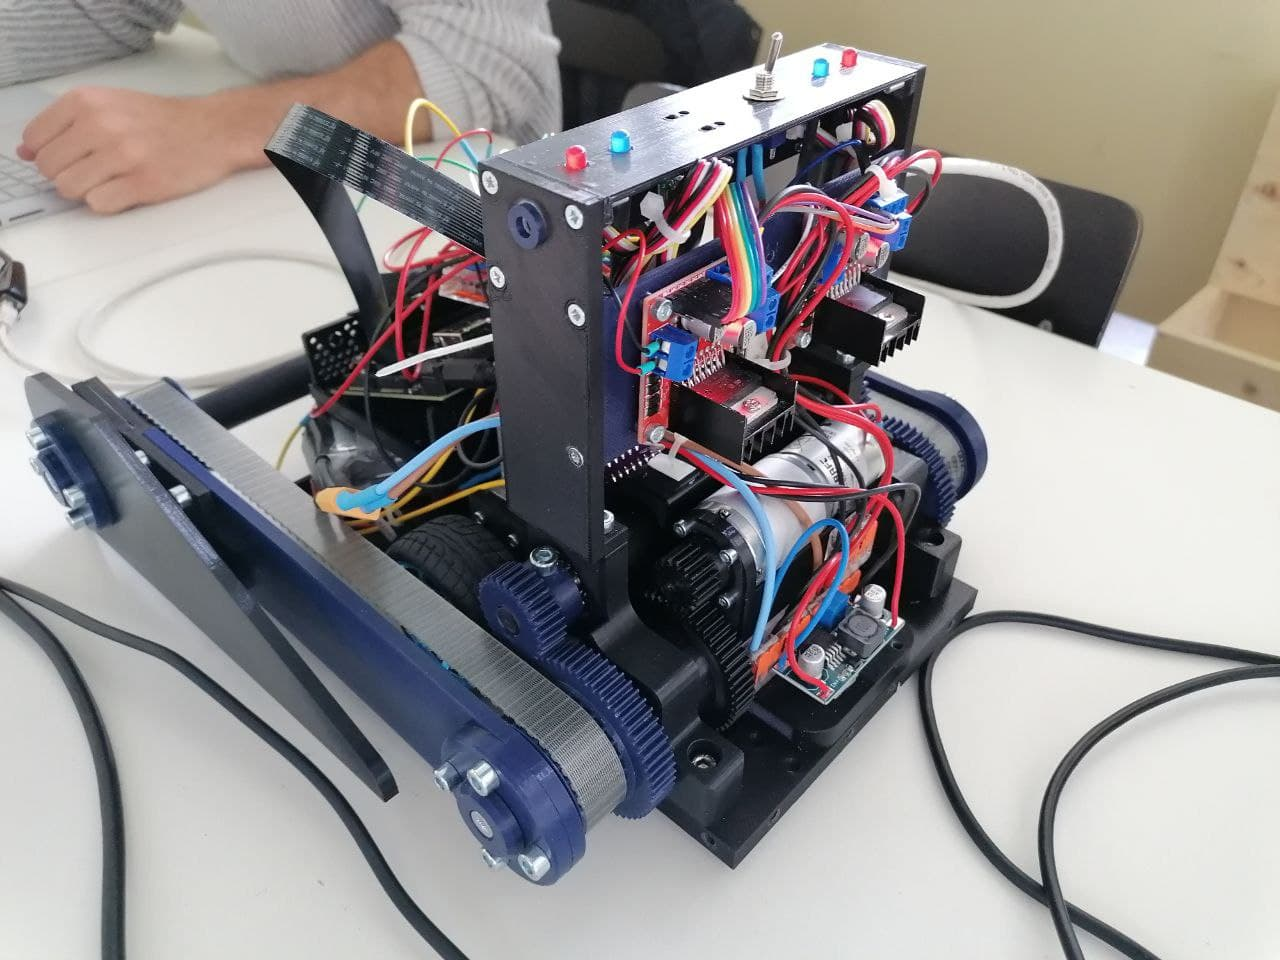
\includegraphics[width=0.65\textwidth]{img/Sprint3/Sprint3_Verkabelung1.jpg}
  \centering
  \caption{Rückansicht der ersten Verkabelung mit Akku}
  \label{fig:Rückansicht der ersten Verkabelung}
  \end{figure}
  
  
  In einem ersten Schritt werden die zwei Spannungslevel hergestellt. Der Akku liefert 16 Volt, welche für alle Motoren verwendet werden. Mithilfe des Wandlers wird das zweite Niveau von 5 Volt erreicht, welches neben dem Jetson auch sämtliche Sensoren unabhängig des Controllers mit Strom versorgt. So kann das Jetson den zur verfügung gestellten Strom für die volle Leistung verwenden.
  Die Verkabelung sämtlicher Elemente ist provisorisch. Geplant ist, dass das Kabelmanagement nach abschluss der Funktionskontrolle aller Elemente verbessert wird um zu einem späteren Zeitpunkt einen besseren Überblick zu gewährleisten.
  
   \begin{figure}[H]
  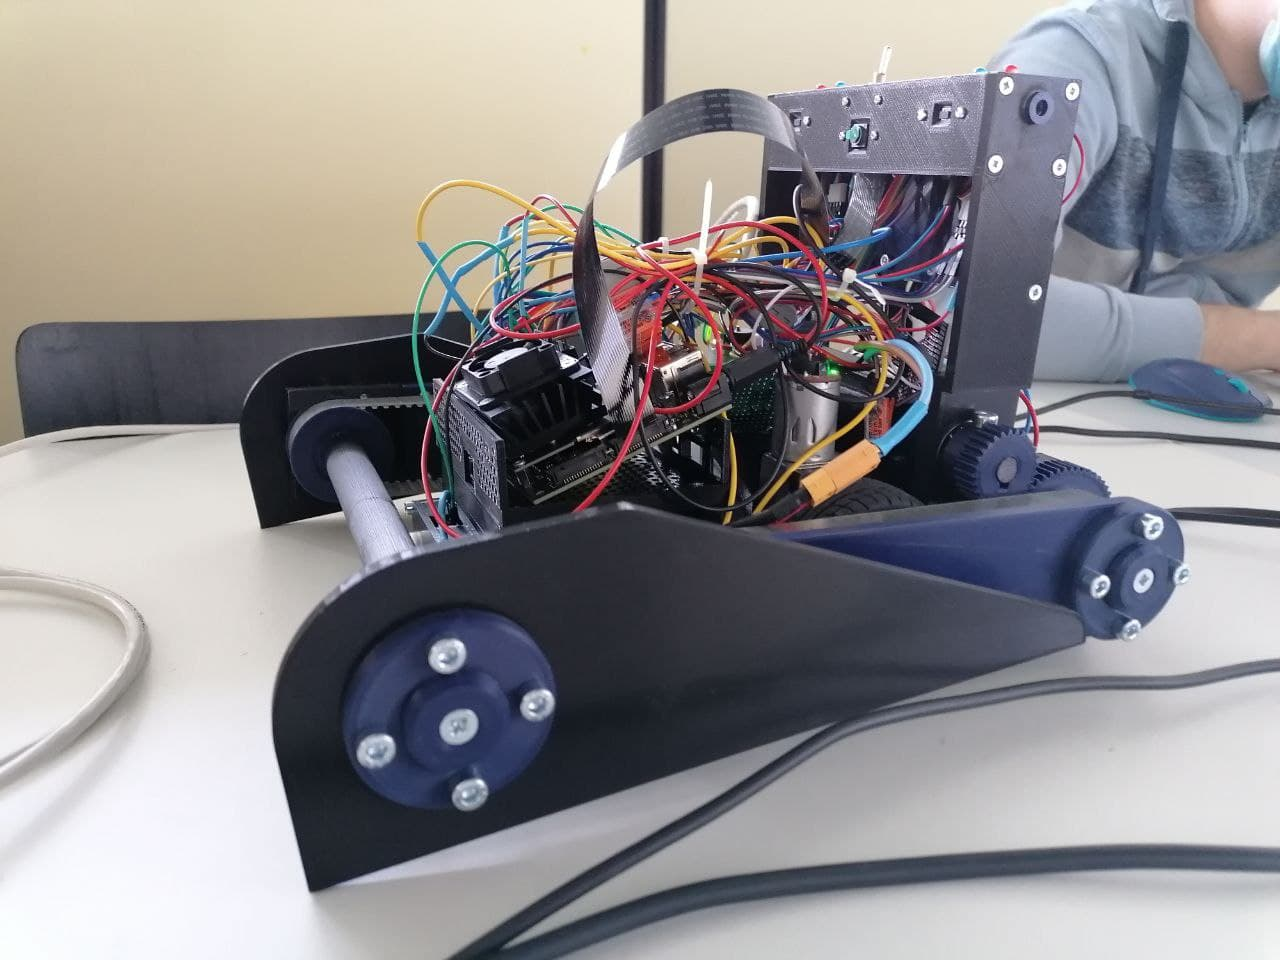
\includegraphics[width=0.65\textwidth]{img/Sprint3/Sprint3_Verkabelung2.jpg}
  \centering
  \caption{Seitenansicht der ersten Verkabelung mit Akku}
  \label{fig:Seitenansicht der ersten Verkabelung}
  \end{figure}
  
  Der Notschalter der fertigen Konstruktion schaltet wie geplant nur die H-Brücken der Motoren. Die 5 Volt Spannungsverteilung wird vom dem Schalter nicht tangiert. Dies um zu umgehen, dass das Jetson Nano ohne korrektes Herunterfahren abgeschaltet wird.
  
  Zusätzlich wurde auch ein Motor zur Hubbewegung entfernt und der Motor zuständig für die erste Hubbewegung weiter zur Spitze verlagert. Somit kann der Gesammtschwerpunkt zusätzlich verbessert werden.
Die Welle des entfernten Motors wird wieder mit einer 3D gedruckten Welle ersetzt um wiederum Gewicht zu sparen. Diese Welle wird korrekt eingestellt und dann fixiert, da die Standsicherheit gegeben ist und das einklappen der Ausleger nicht mehr benötigt wird.
  
 Ergebnisse: Mithilfe der Gewichtsreduktion kann die Hubbewegung schneller und einfacher durchgeführt werden. Das Pathfinding wurde mithilfe der über 300 Referenzbilder trainiert und liefert überzeugende Ergebnisse.
 
 \subsection{Einbindung des Jetson Controller}

 Um das Jetson einbinden zu können, müssen die Module der Software auf die Jetson-Libraries umgeschrieben werden. Dazu werden die Module der State-Machine auf eine GPIO-Librarie, welche vom Jetson unterstützt wird, reduziert. Da das Jetson kein eingebundenes WLAN-Modul besitzt, werden für die Tests ein externes WLAN Modul eingebunden um den Roboter weiterhin remote steuern und updaten zu können.
 
 Zusätzlich wird ein externer PWM Verteiler verwendet, da das Jetson nur über zwei PWM Ausgänge verfügt. Somit können alle Motoren über Hardware-PWM Pins angesteuert werden als im Vergleich zum Raspberry Pi über Software PWMs. 
 
 \section{Softwarearchitektur}
\subsection{Komponentenarchitektur}
Die Software ist objektorientiert und modular aufgebaut. Die verschiedenen Teilfunktionen als auch die Harwaretreiber sind in eigene Komponenten eingebettet. Die Komponenten können über eine schmale vordefinierte Schnittstelle angesprochen werden. Im Bild \ref{fig:komponentenmodell} ist das Komponentenmodell abgebildet. 

\begin{figure}[H]
  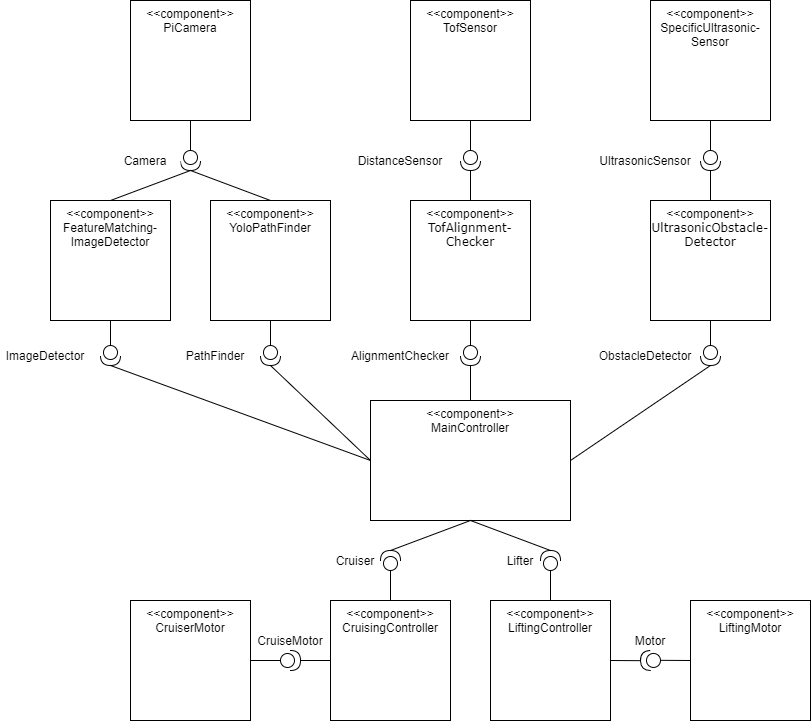
\includegraphics[width=1\textwidth]{img/softwarearchitektur/Softwarearchitektur.png}
  \centering
  \caption{Komponetenmodell}
  \label{fig:komponentenmodell}
\end{figure}

\subsubsection{Main Controller}
Der Main Controller ist der Kern, welche die restlichen Komponenten zielbringend orchestriert. Innerhlab des Main Controllers befindet sich eine Finite State Machine:\\ \texttt{StairClimbingFrog}. Diese ist im Kapitel \ref{sec:fsm} beschrieben. 

In der Abbildung \ref{fig:uml-main} ist zusehen, dass die verschiedenen Zustände und Unterzustände mithilfe von Enumerationen realisiert werden. Dies bring zum einen den Vorteil mit sich, dass man zur Kompilierzeit einen Compileerror erhält, wenn der Zustand nicht existiert. Wären die Zustände mithilfe von Strings realisiert, würde man erst zur Laufzeit erfahren, ob diese Zustände existieren oder nicht. Weiter ist der Workflow dank dem Intellisense, welches durch Enumerationen ermöglicht wird, beschleunigt.

\begin{figure}[H]
  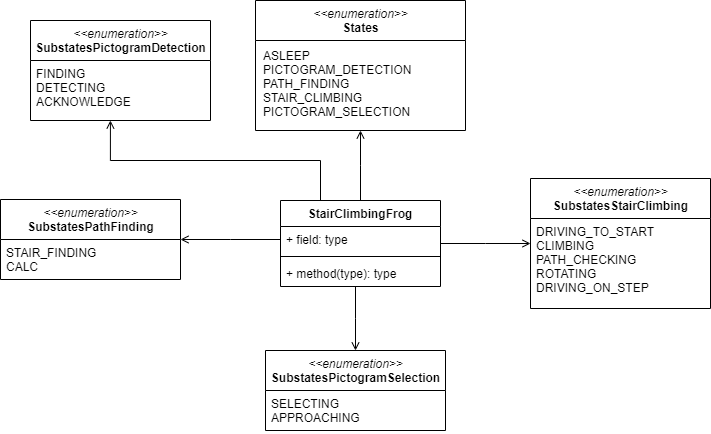
\includegraphics[width=0.95\textwidth]{img/softwarearchitektur/UML-MainController.png}
  \centering
  \caption{UML: MainController}
  \label{fig:uml-main}
\end{figure}


\subsubsection{Lifting Controller}
Der Lifting Controller ist dazu da, den Hauptmotor anzusteuern.
Das Interface \texttt{LiftingMotor} bestimmt die Methoden welche die Hardwaretreiber-Wrapper: \texttt{MainLiftingMotor} und \texttt{AuxilaryLiftingMotor} implementieren sollen. Der LiftingController implementiert das Interface: \texttt{Lifter}. Über dieses Interface kann der \texttt{LiftingController} von aussen angesprochen werden. Weiter hält er die Instanz des Motors.

\begin{figure}[H]
  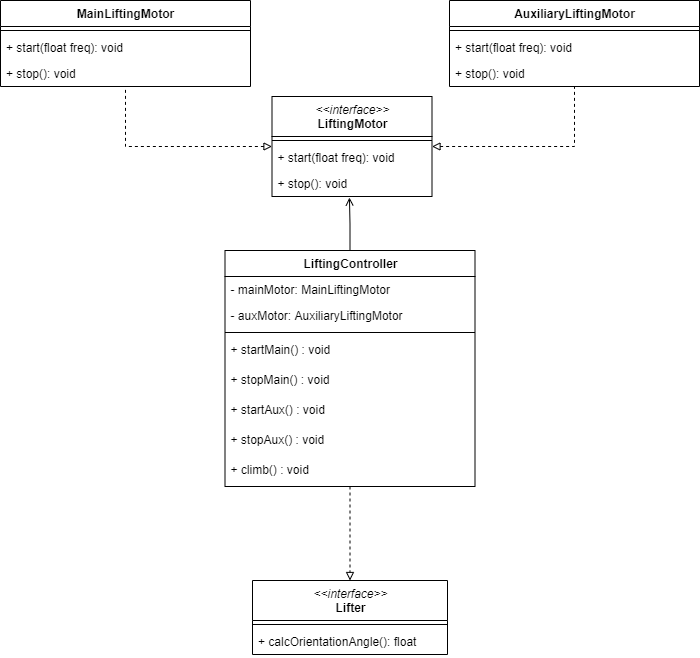
\includegraphics[width=0.95\textwidth]{img/softwarearchitektur/UML-LiftingController.png}
  \centering
  \caption{UML: LiftingController}
  \label{fig:uml-lifting-controller}
\end{figure}


\subsubsection{Cruising Controller}
Die Komponente Cruising Controller ist grundsätzlich gleich aufgebaut wie derLifting Controller. Über das Interface \texttt{CruiseMotor} werden die spezifischen Motorenimplementationen abstrahiert. Der \texttt{CruiseController} hat je eine Instanz vom \texttt{LeftCruiseMotor} und \texttt{RightCruiseMotor}. Über die verschiedenen Methoden, welcher durch das \texttt{Cruiser} Interface vorgegeben werden, kann die Fortbewegung des Roboters gesteuert werden.
\begin{figure}[H]
  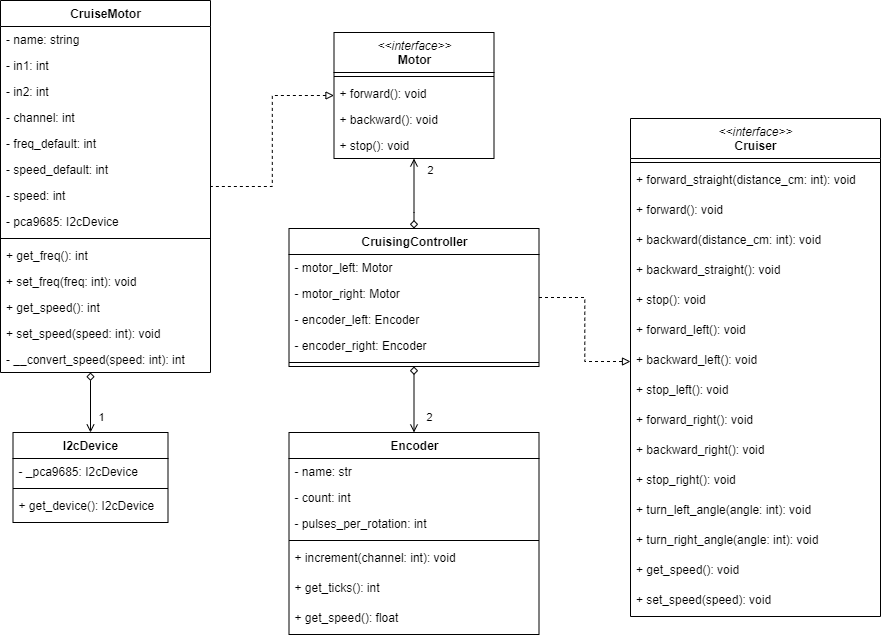
\includegraphics[width=0.95\textwidth]{img/softwarearchitektur/UML-CruisingController.png}
  \centering
  \caption{UML: CruisingController}
  \label{fig:uml-cruising-controller}
\end{figure}

\subsubsection{Tof Alignment Checker}
Der \texttt{TofAlignmentChecker} hält die Instanzen der beiden Tof-Treiber-Wrapper \texttt{LeftTofSensor} und \texttt{RightTofSensor} und liefert die Differenz zurück. Mithilfe dieser Differenz kann sich der \texttt{StairClimbingFrog} senkrecht zur Treppe ausrichten.
\begin{figure}[H]
  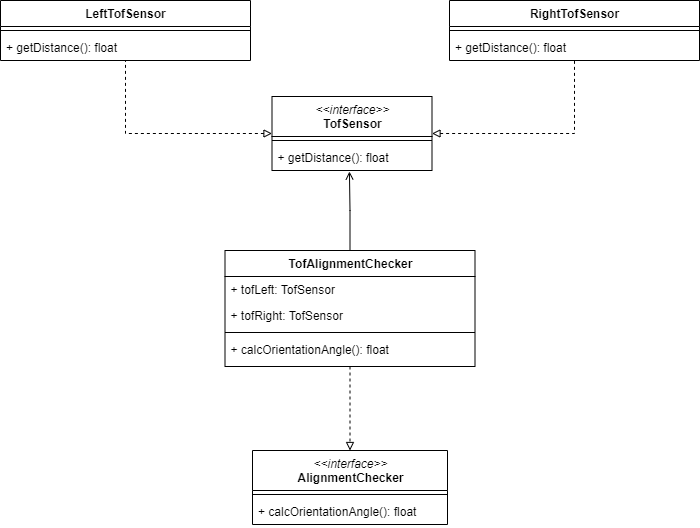
\includegraphics[width=0.95\textwidth]{img/softwarearchitektur/UML-TofAlignmentChecker.png}
  \centering
  \caption{UML: TofAlignmentChecker}
  \label{fig:uml-tof-alignment-checker}
\end{figure}

\subsubsection{Ultrasonic Obstacle Detector}
Ähnlich aufgebaut ist der Ultrasonic Obstacle Detector. Über das Interface \texttt{ObstacleDetector} kann der \texttt{UltrasonicObstacleDetector} angesprochen werden. Dieser erkennt mithilfe seiner Instanzen \texttt{FrontUltrasonicSensor} Hindernisse vor dem Roboter und liefert die Distanz zu diesem zurück.
\begin{figure}[H]
  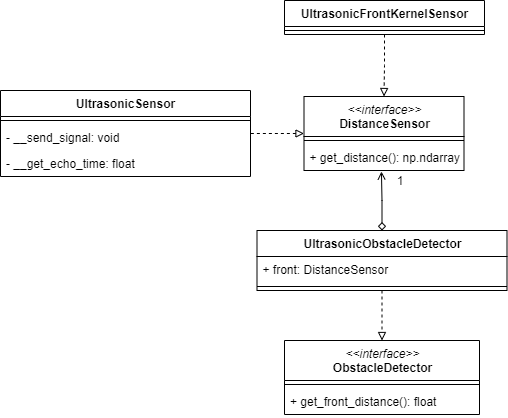
\includegraphics[width=0.95\textwidth]{img/softwarearchitektur/UML-UltrasonicObstacleDetector.png}
  \centering
  \caption{UML: UltrasonicObstacleDetector}
  \label{fig:uml-ultrasonic-obstacle-detector}
\end{figure}

\subsubsection{Feature Matching Image Detector}
\label{sec:architecture-feature-matching}
Die Feature Matching Image Detector Komponente wird verwendet, um das Piktogramm im Startbereich zu finden und zu erkennen. Weiter ist er zuständig, um das richtige Piktogramm im Zielbereich auszuwählen. 
Die Klasse \texttt{Piktogramm} repräsentiert die zu detektierende Piktogramme und deren vorbestimmte Keypoints und Deskriptoren (Features). Der \texttt{SiftImageDetector} implementiert über das Interface \texttt{Camera} eine spezifische Kamera Implementation. Für die Bilder, welche die Kamera macht, werden ebenfalls die Features berechnet und mit diesen der Piktogramme abgeglichen. Der Main Controller kann über das \texttt{ImageDetecotr} Interface die entsprechenden Methoden des \texttt{SiftImageDetector} aufrufen.

\begin{figure}[H]
  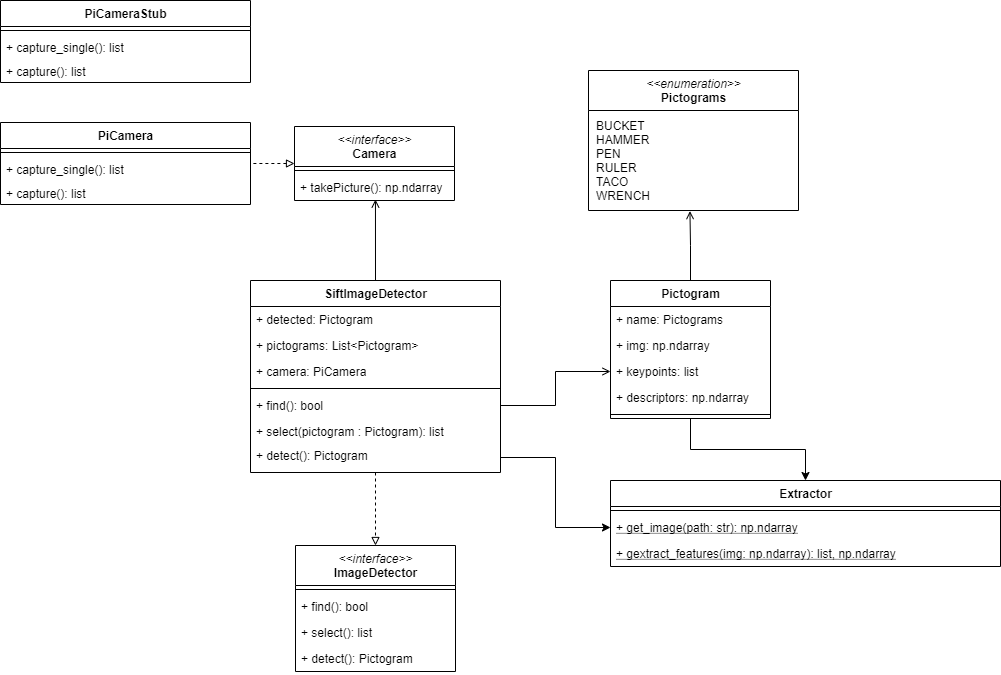
\includegraphics[width=1\textwidth]{img/softwarearchitektur/UML-FeatureMatchingImageDetector.png}
  \centering
  \caption{UML: FeatureMatchingImageDetector}
  \label{fig:uml-feature-matching-image-detector}
\end{figure}

Der \texttt{PiCameraStub} dient lediglich dem Testing. Dem \texttt{SiftImageDetector} kann mittels dependency injection die spezifsiche Kameraimplementation übergeben werden. Die Methoden des Testdoubles liefern vordefinierbare Bilder, welche beim Erzeugen des \texttt{PiCameraStubs} oder danach gesetzt werden können. Im nachfolgenden Codesnippet wird anhand eines Test-Cases die Anwendung des \texttt{PiCameraStubs} veranschaulicht.

\begin{minted}{python}
  class TestSiftImageDetector(unittest.TestCase):
    def test_detect_bucket(self):
        print("\n--- Start test detect bucket ---")
        detectImage = "C:\\git\\hslu-pren\\pren2\\frog\\image_detector\\img\\test\\bucket.jpg"
        selectImage = ""
        stub = PiCameraStub(detectImage, selectImage)
        detector = SiftImageDetector(camera = stub)
        self.assertEqual(detector.detect().name, Pictograms.BUCKET)
    
    ...
 \end{minted}

\subsection{Finite State Machine}
\label{sec:fsm}
Die Main-Komponenten regelt mithilfe einer Finite-State-Machine (FSM) den gessamten Lebenszyklus des Roboters während des Wettbewerbs. In Abbildung \ref{fig:fsm} sind die Hauptzustände modelliert. Innerhalb von jedem Hauptzustand befindet sich eine eigenständige Sub-Statemachine. Die Do-Aktivitäten innerhlab von einem Hauptzusatand werden innerhalb der Unterzustände realisiert. 

\begin{figure}[H]
  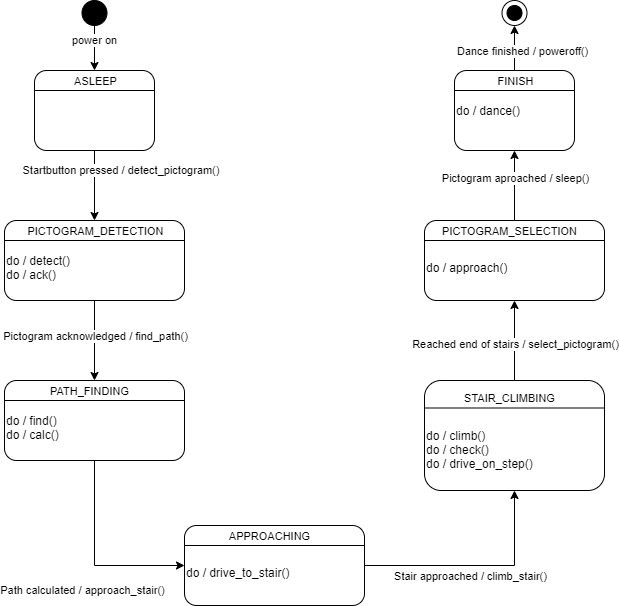
\includegraphics[width=1\textwidth]{img/softwarearchitektur/FSM-FSM.png}
  \centering
  \caption{Finite-State-Machine}
  \label{fig:fsm}
\end{figure}

\begin{figure}[H]
  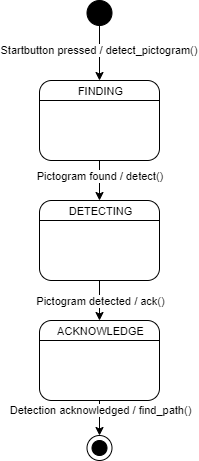
\includegraphics[width=0.40\textwidth]{img/softwarearchitektur/FSM-PICTOGRAM_DETECTION.png}
  \centering
  \caption{FSM: Piktogrammerkennung}
  \label{fig:fsm-pictogrammdetection}
\end{figure}

\begin{figure}[H]
  \includegraphics[width=0.40\textwidth]{img/softwarearchitektur/FSM-PATH_FINDING.png}
  \centering
  \caption{FSM: Pfadfindung}
  \label{fig:fsm-pathfinding}
\end{figure}

\begin{figure}[H]
  \includegraphics[width=1\textwidth]{img/softwarearchitektur/FSM-STAIR_CLIMBING.png}
  \centering
  \caption{FSM: Treppensteigen}
  \label{fig:fsm-stair-climbing}
\end{figure}

\begin{figure}[H]
  \includegraphics[width=0.40\textwidth]{img/softwarearchitektur/FSM-PICTOGRAM_SELECTION.png}
  \centering
  \caption{FSM: Piktogrammauswahl}
  \label{fig:fsm-pictogram-selection}
\end{figure}



\section{Piktogrammerkennung}
Im Abschnitt \ref{sec:architecture-feature-matching} wurde die Feature-Matching-Image-Detector-Komponenten bereits vorgestellt. In diesem Kapitel wird speziell auf das im \texttt{SiftImageDetector} Modul implementierte Feature Matchingverfahren mit OpenCV eingegangen. Es wird der Lösungsweg aufgezeigt, wie die Klassifizierungsgenauigkeit und die Laufzeit-Performance optimiert werden kann.

\subsection{Übersicht Feature Matching}
Als Feature Matching wird ein Verfahren bezeichnet, bei welchem aus einem Bild gewisse Merkmale extrahiert werden. Diese können beispielsweise in einer Datenbank abgespeichert werden. Zu einem späteren Zeitpunkt können diese Merkmale mit jenen eines anderen Bildes abgleichen werden. Stimmen eine gewisse Anzahl dieser überein, so stimmen auch die dazugehörigen Teile der beiden Bilder überein. Dieser Vorgang kann in die nachfolgenden drei Teile unterteilt werden.

\begin{enumerate}
    \item Detektion (Extraktion der Merkmale auch Keypoints genannt)
    \item Deskription (Eindeutige Beschreibung der Merkmale)
    \item Matching (Vergleichen der Merkmale)
\end{enumerate}

Für jeden dieser drei Schritte gibt es verschiedene Algorithmen, welche zum Ziel führen. Gängige Detektoren und Deskriptoren sind z.B. SIFT, ORB, SURF oder MSER. Für das Matching bietet sich das Bruteforce Matching oder ein FLANN basiertes Matching an. Nachfolgend werden die alle Algorithmen mit welchen Tests durchgeführt wurden kurz aufgelistet und grob erklärt.

\subsubsection{Scale Invariant Feature Matching (SIFT)}

\subsubsection{Oriented Fast and Rotated BRIEF (ORB)}

\subsubsection{Fast Library for Approximate Nearest Neighbours (FLANN)}

\subsection{Genauigkeit}
Es wurde festgestellt, dass ab einer gewissen Entfernung des Piktogramms die Anzahl guter Matches stark abnimmt. Es wurde ebenfalls festgestellt, dass wenn man das Piktogramm heranzoomt und so weniger Hintergrund vorhanden war, die Genauigkeit erhöht wurde. Dies führte zum Schluss, dass grosse Hintergrundflächen die Ergebnisse negativ beeinflussen. Da man jedoch nicht gewillt war, die Einbussen in der Sichtweite, welche durch den Zoom verursacht werden, in kauf zu nehmen, hat man versucht den Region of Interes (ROI) vor der Detektion einzugrenzen. Als aller erstes wurden jedoch verschiedene Algorithmen für die Detektion und Deskription ausprobiert. Um den ROI einzugrenzen wurde versucht das Bild für die Detektion in mehrere Teile zu zerlegen. Weiter wurde versucht mithilfe von Histogram Backprojection abzuschätzen, wo sich das Piktogramm in etwa befinden könnte.

\subsubsection{Vergleich SIFT vs. ORB}
\textbf{ORB}\\

\begin{figure}[H]
  \centering
  \begin{minipage}[t]{0.45\linewidth}
  \includegraphics[width=1.0\textwidth]{img/piktogrammerkennung/orb_kp1.jpg}
  \caption{Extrahierte Merkmale mit ORB vom Template}
  \label{fig:orb-kp1}
  \end{minipage} 
  \hfill
  \begin{minipage}[t]{0.45\linewidth}
  \includegraphics[width=1.0\textwidth]{img/piktogrammerkennung/orb_kp2.jpg}
  \caption{Extrahierte Merkmale mit ORB vom Inputbild}
  \label{fig:orb-kp2}
  \end{minipage}
\end{figure}

\begin{figure}[H]
  \includegraphics[width=0.95\textwidth]{img/piktogrammerkennung/orb_matches.jpg}
  \centering
  \caption{Matches der ORB Merkmale mit einem Matchverhältniss von 0.75}
  \label{fig:orb-matches-0.75}
\end{figure}

\begin{figure}[H]
  \includegraphics[width=0.95\textwidth]{img/piktogrammerkennung/orb_matches_0.85.jpg}
  \centering
  \caption{Matches der ORB Merkmale mit einem Matchverhältniss von 0.85}
  \label{fig:orb-matches-0.85}
\end{figure}

Matching Results\\
*******************************\\
\# Keypoints 1:                           388\\
\# Keypoints 2:                           1903\\
\# Matches:                               388\\
\# Good Matches:                          0\\

\textbf{SIFT}\\

\begin{figure}[H]
  \centering
  \begin{minipage}[t]{0.45\linewidth}
  \includegraphics[width=1.0\textwidth]{img/piktogrammerkennung/sift_kp1.jpg}
  \caption{Extrahierte Merkmale mit SIFT vom Template}
  \label{fig:sift-kp1}
  \end{minipage} 
  \hfill
  \begin{minipage}[t]{0.45\linewidth}
  \includegraphics[width=1.0\textwidth]{img/piktogrammerkennung/sift_kp2.jpg}
  \caption{Extrahierte Merkmale mit SIFT vom Inputbild}
  \label{fig:sift-kp2}
  \end{minipage}
\end{figure}

\begin{figure}[H]
  \includegraphics[width=0.95\textwidth]{img/piktogrammerkennung/sift_matches.jpg}
  \centering
  \caption{Matches der SIFT Merkmale mit einem Matchverhältniss von 0.7}
  \label{fig:orb-matches-0.75}
\end{figure}

Matching Results \\
*******************************\\
\# Keypoints 1:                           31\\
\# Keypoints 2:                           233\\
\# Matches:                               31\\
\# Good Matches:                          3\\

\subsubsection{ROI Eingrenzung mittels Histogramm Backprojection}
Bei der Histogramm Backprojection wird ganz grob gesagt, ein Bild erzeugt, bei welchem jedes Pixel die Wahrscheinlichkeit angibt, dass es zum vorgegebenen Template gehört. Ist es zu 100\% wahrscheinlich, dass das Pixel im Inputbild zu einem vorgegebenen Template gehört, wird erhält dies z.B. den Wert 255. Desto weniger gross die Chance ist, desto kleiner wird der Graustufenwert des Pixels.

Diese resultierende Wahrscheinlichkeitsmatrix kann man mithilfe von Thresholding zu einer Maske machen und mit dem Inputbild Multiplizieren oder auch bitweise Und-Verknüpfen. Dann erhält man nur die Stellen des Inputbildes, welche zu einer gewisse Wahrscheinlichkeit (welche beim Thresholding festgelegt wird) zum Template gehören. 

Das Ziel war es also, ahnahnd dieser Maske herauszufinden, auf welche Stelle im Inputbild gezoomt werden soll. So wird verhindert, dass man aus versehen die Stelle welche das Piktogramm beinhaltet wegschneidet.

Auf dem Bild \ref{fig:backprojection-hammer} sind die drei oben beschriebenen Schritte visualisiert. Ganz links ist das Inputbild zu sehen, in der Mitte die Maske welche sich aus der Wahrscheinlichkeitsmatrix ergeben haben. Ganz rechts ist das Resultat aus der Multiplikation von der Maske mit dem Inputbild zu sehen. Als Template wurde das Piktogramm auf folgender Abbildung \ref{fig:sift-kp1} verwendet. Bereits in der Maske aber vorallem auch im Bild ganz rechts ist zu sehen, dass das Piktogramm nicht erkannt wurde. 

\begin{figure}[H]
  \includegraphics[width=1\textwidth]{img/piktogrammerkennung/hammer_backprojection.jpg}
  \centering
  \caption{Histogramm Backprojection vom Hammer Piktogramm}
  \label{fig:backprojection-hammer}
\end{figure}

Da der selbe Programmcode auf einem anderen Bild viel bessere Resultate erzielte, wurde dieser Ansatz verworfen. Das Bild \ref{fig:backprojection-hand} zeigt, dass der grüne Hintergrund ziemlich gut von den Händen differenziert werden konnten. Ein Grund für die schlechten Ergebnisse mit dem Piktogramm als Template kann sein, dass diese lediglich schwarze und weisse Pixel beinhalten und der Hintergrund des Inputbildes ebenfalls wenig unterschiedliche Farben enthält. Der Algorithmus für die Histogramm Backprojection arbeitet jedoch mit dem HSV-Wert. Somit ist es möglich, dass die HSV-Werte zu wenig grosse Unterschiede aufweisen, als dass diese ohne aufwändiges Finetuneing der Hyperparameter deutlich unterschieden werden können. Wenn man jedoch ein grünes Pixel (HSV: 120) von einem Roten Pixel (HSV: 0) unterscheiden muss, ist dies einfacher, da die Differenz zwischen den HSV-Werten viel deutlicher ist. 

\begin{figure}[H]
  \includegraphics[width=1\textwidth]{img/piktogrammerkennung/hand_backprojection.jpg}
  \centering
  \caption{Histogramm Backprojection vom gut geeignetem Bild}
  \label{fig:backprojection-hand}
\end{figure}


\subsection{ROI Eingrenzung mittels Konturenerkennung}
Um die Genauigkeit des Feature Matching zu erhöhen, wurde eine Idee welche in PREN1 entstanden ist umgesetzt. Das Bild soll auf rechteckige Konturen abgesucht werden. Dabei werden die gefundenen Konturen nach ihrer Fläche sortiert. Man geht dann davon aus, dass es sich beim Rechteck mit der grössten Fläche um das Piktogramm handelt. 

In Abbildung \ref{fig:contour-hammer} ist zu sehen, dass der Algorithmus keine rechteckigen Konturen auf dem Bild mit dem Hammerpiktogramm erkennen konnte. Das Problem ist in Bild \ref{fig:edge-hammer} zu sehen. Die Kanten des Piktogramms werden nicht richtig erkannt. Dies könnte daran liegen, dass die Halterung ebenfalls Weiss ist. Was einen sehr geringen Kontrast zur folge hat und dieser Geringe Kontrast liefert nur sehr flache Gradienten, welche schlussendlich in keiner oder nur einer löchrigen Kante resultieren. Auch durch Tuneing der Parameter der Kantenerkennung, wurden keine konstant besseren Resultate erzielt.

\begin{figure}[H]
  \centering
  \begin{minipage}[t]{0.45\linewidth}
  \includegraphics[width=1.0\textwidth]{img/piktogrammerkennung/edge_hammer.jpg}
  \caption{Kantenerkennung des Hammers}
  \label{fig:edge-hammer}
  \end{minipage} 
  \hfill
  \begin{minipage}[t]{0.45\linewidth}
  \includegraphics[width=1.0\textwidth]{img/piktogrammerkennung/contours_hammer.jpg}
  \caption{Erkannte Rechteckige Konturen des Hammers}
  \label{fig:contour-hammer}
  \end{minipage}
\end{figure}

Derselbe Algorithmus wurde an einem Beispielbild getestet, welches klare Kanten beinhaltet, welche steile Gradienten zur folge haben. Auf dem nachfolgenden Bild \ref{fig:scanned-doc} sind die Resultate abgebildet. So konnte sichergestellt werden, dass der Algorithmus theoretisch zum gewünschten Ergebnis führt.

\begin{figure}[H]
  \centering
  \begin{minipage}[t]{0.32\linewidth}
  \includegraphics[width=1.0\textwidth]{img/piktogrammerkennung/edge_doc.jpg}
  \caption{Kantenerkennung des optimalen Testbildes}
  \label{fig:edge-doc}
  \end{minipage} 
  \hfill
  \begin{minipage}[t]{0.32\linewidth}
  \includegraphics[width=1.0\textwidth]{img/piktogrammerkennung/contours_doc.jpg}
  \caption{Erkannte Rechteckige Konturen des optimalen Testbildes}
  \label{fig:contour-doc}
  \end{minipage}
  \hfill
  \begin{minipage}[t]{0.32\linewidth}
  \includegraphics[width=1.0\textwidth]{img/piktogrammerkennung/scanned_doc.jpg}
  \caption{ROI Eingrenzung des optimalen Testbildes}
  \label{fig:scanned-doc}
  \end{minipage}
\end{figure}

\subsubsection{Bild für Detektion in Teilbilder aufteilen}
\label{sec:detektion-auf-teilbildern}
Da man davon ausgegangen ist, das viel Hintergrundfläche einen negativen Einfluss auf die Matchergebnisse hat, war die Idee, das Bild in mehere Teilbilder aufzuteilen. Auf den einzelnen Teilbildern werden dann die Keypunkte extrahiert. Diese Keypunkte werden dann für die Deskription und das Matching auf das gesamte Bild abgetragen.

\begin{figure}[H]
  \centering
  \begin{minipage}[t]{0.22\linewidth}
  \includegraphics[width=1.0\textwidth]{img/piktogrammerkennung/slice0_kp2.jpg}
  \caption{Extrahierte Merkmale mit SIFT von Slice 0}
  \label{fig:slice0-kp2}
  \end{minipage} 
  \hfill
  \begin{minipage}[t]{0.22\linewidth}
  \includegraphics[width=1.0\textwidth]{img/piktogrammerkennung/slice1_kp2.jpg}
  \caption{Extrahierte Merkmale mit SIFT von Slice 1}
  \label{fig:slice1-kp2}
  \end{minipage}
  \hfill
  \begin{minipage}[t]{0.22\linewidth}
  \includegraphics[width=1.0\textwidth]{img/piktogrammerkennung/slice2_kp2.jpg}
  \caption{Extrahierte Merkmale mit SIFT von Slice 2}
  \label{fig:slice2-kp2}
  \end{minipage}
  \hfill
  \begin{minipage}[t]{0.22\linewidth}
  \includegraphics[width=1.0\textwidth]{img/piktogrammerkennung/slice3_kp2.jpg}
  \caption{Extrahierte Merkmale mit SIFT von Slice 3}
  \label{fig:slice3-kp2}
  \end{minipage}
\end{figure}

\begin{figure}[H]
  \includegraphics[width=0.95\textwidth]{img/piktogrammerkennung/sift_kp2_from_slice.jpg}
  \centering
  \caption{Matches der ORB Merkmale mit einem Matchverhältniss von 0.85}
  \label{fig:sift-kp2-slice}
\end{figure}

Um die Merkmale auf das uhrsprüngliche Bild zu übertragen, müssen zu deren x-Koordinaten in diesem Fall 100px bzw. 200px bzw. 300px hinzuaddiert werden. Diese 100px ergeben sich daraus, dass das Bild auf 400px Breite skaliert wurde und in vier Streifen von je 100px Breite geschnitten wurde. Hierbei hat sich gezeigt, dass sich die Werte beim anpassen teilweise scheinbar sporadisch leicht ändern. 

Zum Beispiel hat man zu dem Merkmal (6.106937408447266, 81.14856719970703) welches sich im zweiten Slice befindet 100 hinzuaddiert. Nach der Addition scheint der Wert noch zu stimmen: [106.10693740844727, 81.14856719970703]. Nach der Konvertierung in ein Tupel noch immer: (106.10693740844727, 81.14856719970703). Doch sobald die neue Koordinate effektiv dem \texttt{KeyPoint} zugewiesen wurde, stimmt der Wert ab der 6. Nachkommastelle nicht mehr überein: (106.10693359375, 81.14856719970703).

Bei anderen Merkmalen, scheint dies jedoch nicht der Fall zu sein:

(38.83573913574219, 117.7967529296875)\\
(138.8357391357422, 117.7967529296875)\\
(138.8357391357422, 117.7967529296875)\\
(138.8357391357422, 117.7967529296875)\\

Nachfolgend ein Auschnitt des Programmcodes, welcher zu den Keypunkten den entsprechenden Wert hinzuaddiert und von dem auch die obigen Koordinaten ausgegeben wurden:

\begin{minted}{python}
    for kp in kp2[1]:
        nkp = list(kp.pt)
        print(kp.pt)
        nkp[0] = nkp[0] + 100
        print(nkp)
        print(tuple(nkp))
        kp.pt = tuple(nkp)
        print(kp.pt)
    for kp in kp2[2]:
        nkp = list(kp.pt)
        nkp[0] = nkp[0] + 200
        kp.pt = tuple(nkp)
    for kp in kp2[3]:
        nkp = list(kp.pt)
        nkp[0] = nkp[0] + 300
        kp.pt = tuple(nkp)
    kp2 = list(chain.from_iterable(kp2))
\end{minted}

Aufjedenfall, scheint sich diese sporadische Datenkorruption negativ auf die Matchergebnisse auszuwirken. In der Abbildung \ref{fig:sift-matches-slice} ist zu sehen, dass die gematchten Keypunkte nicht mehr zum Piktogramm gehören. 

\begin{figure}[H]
  \includegraphics[width=0.95\textwidth]{img/piktogrammerkennung/sift_matches_slice.jpg}
  \centering
  \caption{Matches der SIFT Merkmale aus den verschiedenen Slices mit einem Matchverhältniss von 0.7}
  \label{fig:sift-matches-slice}
\end{figure}

Das oben geschilderte Problem wurde unter anderem nicht mehr weiter untersucht, da beim Auswerten der Anzahl guter Matches aufgefallen ist, dass sich diese in der Anzahl nicht unterscheiden. Ohne Slicing wurde die gleiche Anzahl Matches gefunden wie mit Slicing. Dies löste jedoch den verdacht aus, dass die gefundene Anzahl positiver Matches nicht von der Fläche des unrelevanten Hintergrundes abhängt, sondern von der Skalierung des Bildes. Den bei einem Zoom, bzw. beim wegschneiden des Hintergrundes, wird nicht nur die Hintergrundfläche minimiert, sondern auch automatisch die Skalierung des Piktogramms verändert. Dies aus dem Grund, weil das Inputbild als auch das Template zu beginn des Matchings auf fixe 400 px breite skaliert wird.

Matching Results\\
*******************************\\
\# Keypoints 1:                           31\\
\# Keypoints 2:                           218\\
\# Matches:                               31\\
\# Good Matches:                          3\\

\subsubsection{Skalierung}
Wie bereits am Ende des Kapitels \ref{sec:detektion-auf-teilbildern} beschrieben. Kann es sein, dass nicht die Grösse der unrelevanten Hintergrundfläche die positiven Matches negativ beeinflussen, sondern die Skalierung des Piktogramm selber. Da beide Bilder fix auf 400px Breite skaliert werden, ist das Piktogramm im Inputbild oftmals deutlich kleiner als das Piktogramm im Template. 

Im Bild \ref{fig:sift-matches-800} sind die Ergebnisse zu sehen, wenn das Inputbild lediglich auf 800px Breite skaliert wird und nicht mehr auf 400px wie das Template. Wie vermutet liefert SIFT deutlich bessere Ergebnisse, wenn der Skalierungsunterschied vom Template zum Objekt im Inputbild nicht all zu gross ist. Obwohl es sich bei SIFT und ein Scale Invariantes verfahren handelt, was so viel heisst wie, dass sich die Keypunkte und deren Deskriptoren aufgrund von Skalierung nicht verändern, erzielt man bessere Resultate mit einer grösseren Skalierung des zu detektierenden Objektes. Der Grund dafür ist in den Matching Resultaten zu sehen. Bei einer Skalierung von 800 px werden deutlich mehr Keypunte extrahiert, die Chance auf eine grössere Anzahl positiver Matches steigt also logischerweise an.

\begin{figure}[H]
  \includegraphics[width=0.95\textwidth]{img/piktogrammerkennung/sift_matches_800.jpg}
  \centering
  \caption{Matches der SIFT Merkmale bei einer Skalierung des Inputbildes auf 800px}
  \label{fig:sift-matches-800}
\end{figure}

Matching Results\\
*******************************\\
\# Keypoints 1:                           31\\
\# Keypoints 2:                           400\\
\# Matches:                               31\\
\# Good Matches:                          13\\

\subsection{Performance}




\section{Hinderniserkennung}

Wie bereits im \acrshort{pren1} klar wurde, ist das Problem der Hinderniserkennung zu komplex,
um mit simpler Bildverarbeitung gelöst werden kann. 
Das Erkennen von Objekten auf einem Bild, wurde bereits durch \acrfull{cnn} gelöst.

\subsection{Objektdetektierung mit \acrshort{cnn}}

Die Objektdetektierung ist eines von vier Grundproblemen des {\it Computer Vision} Forschungsbereiches.
Dazu zählen die Bildklassifizierung, Objektdetektierung, Semantische Segmentation und Instance Segmentation.

\image{img/CNN/computer-vision-research-fields}
{
Der Forschungsbereich der {\it Computer Vision} \cite{wu2019recent} besteht aus Bildklassifizierung, 
Objektdetektierung, Semantische Segmentation und Instance Segmentation.
}

Bei der Objektdetektierung werden einzelne Objekte einer bestimmten Klasse mit {\it Bounding Boxes}
eingezeichnet. Die Genauigkeit solcher \acrshort{cnn} kann für ein spezialisiertes Gebiet die
eines Menschen übertreffen \cite{BUETTIDINH2019e00321}.

\subsection{Algorythmen zur Objektdetektierung}

Es gibt verschiedene Algorithmen zur detektierung von Objekten in einem Bild. 
Dabei ist vor allem die Abwägung zwischen Genauigkeit und Geschwindigkeit entscheidend.
Aus diesem Grund wird die Objektdetektierung auch in zwei Gruppen unterteilt, nähmlich 
(i) single-stage detection wie \acrshort{yolo} \cite{redmon2016look} oder \acrshort{ssd} \cite{Liu_2016} und (ii) two-stage detection wie \acrfull{r-cnn} \cite{girshick2015fast}.

Ein two-stage detector besteht aus einem ersten Feature Proposal Schritt, gefolgt von einer Klassifizierung der 
vorgeschlagenen Features des ersten Schrittes. Ein sigle-stage detector klassifiziert die Regionen eines Bildes
direkt in einem Durchlauf. 

Während single-stage Detektoren generell eine schnellere Inference bieten, sind two-stage Detektoren genauer \cite{soviany2018optimizing}.
Aus diesem Grund werden häufig für Real-Time Objektdetektierung, wie das Erkennen von Objekten in einem Videostream, single-stage
Detektoren verwendet.

\subsection{\acrfull{r-cnn}}

Aufgrund der erhöhten Genauigkeit von two-stage Detektoren, wurde in dieser Arbeit vor allem \acrshort{r-cnn} angeschaut.

Bei einem \acrshort{r-cnn} \cite{girshick2014rich} werden zuerst interessante Regionen von einem \acrshort{cnn} für die 
spätere Segmantische Kategorisierung vorgeschlagen. Laut dem Paper von \acrshort{r-cnn}, wird eine um 30\% erhöhte Genauigkeit 
gegenüber vorherigen Objekterkennungsalgorythmen auf dem VOC 2012 Datenset erreicht. Damit wird eine \acrfull{map} von 53.3\%
auf dem VOC 2012 Datenset erreicht.

Bei einem \acrshort{r-cnn} 

\image{img/CNN/r-cnn}
{
  Der \acrfull{r-cnn} \cite{girshick2014rich} Objektdetektierungs Algorythmus bei welchem zuerst Regionen 
  vorgeschlagen werden, auf denen danach mit einem Backbone Segmantische Kategorisierung durchgeführt wird und
  das Objekt einer Klasse zugeteilt wird.
}

\subsection{Erkennung von Ziegelsteinen und Treppenstufen}

\subsubsection{Vereinfachtes \acrshort{r-cnn}}

Ein erster simpler versuch die Hindernisse (Ziegelsteine) zu erkennen war, mittels Feature Engineering\footnote{
In diesem Fall wurde Canny Edge detection \cite{canny-edge-detection} angewendet}, die Treppenstufen zu
erkennen. Ein Sliding Window auf der Treppenstufe dient dabei als Feature Proposal.
Die Kategorisierung wurde mit einem einfachen \acrshort{cnn} basierend auf den Sliding Window features 
gemacht.

\image{img/CNN/sliding-window-stair}
{
Ansatz eines vereinfachten \acrshort{r-cnn} mit Stufenerkennungs Feature engineering.
}

Die Resultate konnten weder die erwartete Performanz noch Genauigkeit zufriedenstellen.
Das Paper dazu kann auf GitHub \footnote{
https://github.com/randombenj/hslu-pren/blob/a987e1c53f3b44a86b42ca3030afb1f12880d94c/pren1/research/yes-no-classification-sliding-window.ipynb} gefunden werden \ref{sec:r-cnn-paper}.


\subsubsection{Detectron2}

Detectron2 \cite{wu2019detectron2} ist ein State of the Art Framework für Objektdetektierung, Semantische- und Instance Segmentierung.
Es werden verschiedene \acrshort{r-cnn} Models zur verfügung gestellt. \footnote{
https://github.com/facebookresearch/detectron2/blob/master/MODEL\_ZOO.md\#coco-object-detection-baselines
}
Zudem bietet Detectron2 eine sehr einfache Möglichkeit mittels Transfer Learning \footnote{\url{https://colab.research.google.com/drive/16jcaJoc6bCFAQ96jDe2HwtXj7BMD_-m5#scrollTo=b2bjrfb2LDeo}}
einen eigenen Datensatz, bestehend auf dem vortrainierten Gewichten der Features zu trainieren.
Somit ist es möglich mit wenigen hundert Bildern neue Objekte zu erkennen.

\subsubsection{Performance Testing}

Um zu sehen ob ein Raspberry Pi solch komplexes \acrshort{cnn} überhaupt berechnen kann, oder ob ein
Leistungsfähigeres Compute Board gekauft werden muss, wurden Performance Tests durchgeführt.
Das setup für die Performance tests kann auf GitHub \footnote{\url{https://github.com/randombenj/detectron2onnx-inference/blob/master/detectron2-onnx.ipynb}} gefunden werden.

Für die Performance Tests wurden drei Controller angeschaut, die Controller konnten ausgeliehen werden.

\begin{itemize}
    \item Raspberry Pi
    \item Jetson Nano (4GB)
    \item Jetson TX1
\end{itemize}

\image{img/CNN/boards}{
Das Jetson TX1 (unten), Jetson Nano (oben mitte) und das Raspberry Pi (oben rechts und links)
}

Die Performance tests wurden mit dem oben genannten Notebook gemacht, zusätzlich wurde die Zeit für die
Inference gemessen. Die Resultate haben eine Inference Zeit ergeben von:

\begin{itemize}
    \item {\bf Raspberry Pi}  ~500s
    \item {\bf Jetson Nano (4GB)} ~10s
    \item {\bf Jetson TX1} ~2s
\end{itemize}

Zwar konnte mit optimierung (durch das einsetzen von ONNX)\footnote{https://onnx.ai/} beim Raspberry Pi eine Inference Zeit von ~20s erreicht werden, 
dann sind aber alle vier CPU Kerne zu 100\% für die gesammte Zeit ausgelastet.

Da die Nvidia Boards jeweils über eine Maxwell GPU verfügen und diese auch mit CUDA \footnote{https://developer.nvidia.com/cuda-zone}
für Machine Learning verwendet werden kann, wurde entschieden, das Jetson Nano anstatt das ursprünglich geplante
Raspberry Pi zu kaufen. Das Jetson Nano verfügt über die gleichen Kamera und GPIO anschlüsse, und 
ist so Kompatibel mit der geplanten Elektronik.

\subsection{Trainieren des \acrshort{cnn}}

Bei den detectron2 \acrshort{cnn} Modellen kann bereits vor trainiertes Neuronales Netz
verwendet werden. Dieses kann danach mit wenigen hundert Bildern via Transfer Learning \footnote{https://en.wikipedia.org/wiki/Transfer\_learning}
auf ein eigenes Datenset angepasst werden.

Den Vorgang kann man sich so vorstellen, dass das Modell verschiedene, häufig vorkommende Formen wie Kreise, Vierecke, ...
bereits kennt und man durch das Datenset dem Modell beibringt was eine Treppenstufe oder ein Ziegelstein ist.

\subsubsection{Sammeln von Trainingsdaten}

Die Trainingsdaten wurden mithilfe eines Kartonprototypen und einer kleinen App gesammelt.
Im Kartonprototypen wurde die Kamera auf der gleichen Höhe und im gleichen Winkel eingebaut
wie im endgerät.
Mithilfe der App auf dem gerät, konnten über das Smartphone einfach Bilder aufgenommen werden.

Die Bilder wurden in einer Auflösung von 720x960px aufgenommen. Ziel war es etwa 300 Bilder zu sammeln um für das \acrshort{cnn} zu annotieren.

\image{img/CNN/pren-image-capture}{
Aufnahme der Trainingsdaten für die Hinderniserkennung
}

\subsubsection{Annotieren der Trainingsdaten}

Die Trainingsdaten wurden nach dem Aufnehmen mithilfe von COCO Annotator \footnote{https://github.com/jsbroks/coco-annotator} annotiert.
Dabei wurden zwei Klassen verwendet: {\it Brick} und {\it Stair}.

\image{img/CNN/coco-stair}{
Annotieren der Trainingsdaten im COCO Datenformat \footnote{\url{https://cocodataset.org/#format-data}}.
}

\subsubsection{Trainieren des \acrshort{cnn}}

Als vorlage für das Trainieren wurde das offizielle Notebook von detectron2 verwendet. \cite{detectron2-colab}

Um das \acrshort{cnn} zu trainieren und auch die Performance zu evaluieren, werden die annotierten Trainingsdaten
in Train- (70\%), Test- (20\%) und Validationsset (10\%) unterteilt.

Die Trainingsdaten dienen dazu das Model zu trainieren, mit den Testdaten werden die Hyperparameter\footnote{\url{https://en.wikipedia.org/wiki/Hyperparameter_(machine_learning)}} verfeinert und
mit dem Validationsset wird am schluss die Performance des \acrshort{cnn} gemessen.

Die verschiedenen Datensätze werden dem detectron2 trainer bekanntgegeben:

\begin{minted}{python}
from detectron2.data.datasets import register_coco_instances

DatasetCatalog.clear()

register_coco_instances("stair_train", {}, "stair-train.coco.json", "stair/")
register_coco_instances("stair_test", {}, "stair-test.coco.json", "stair/test/")
register_coco_instances("stair_validation", {}, "stair-validation.coco.json", "stair/validation/")
\end{minted}

Das Model wurde wie folgt vorkonfiguriert:

\begin{minted}{python}
model_config = "COCO-Detection/faster_rcnn_R_50_FPN_3x.yaml"

cfg = get_cfg()

cfg.merge_from_file(model_zoo.get_config_file(model_config))
cfg.MODEL.ROI_HEADS.SCORE_THRESH_TEST = 0.5  # set threshold for this model

# Use the pretrained model for transfer learning
cfg.MODEL.WEIGHTS = model_zoo.get_checkpoint_url(model_config)

cfg.INPUT.MAX_SIZE_TRAIN = 480
cfg.INPUT.MAX_SIZE_TEST = 480

cfg.OUTPUT_DIR = '480_output'
cfg.DATASETS.TRAIN = ("stair_train",)
cfg.DATASETS.TEST = ("stair_test",)

cfg.DATALOADER.NUM_WORKERS = 2
cfg.SOLVER.IMS_PER_BATCH = 2
cfg.SOLVER.BASE_LR = 0.02
cfg.SOLVER.MAX_ITER = 900

cfg.MODEL.ROI_HEADS.NUM_CLASSES = 2  #  classes (stair, brick)
\end{minted}

Nun kann das Model trainiert werden:

\begin{minted}{python}
trainer = DefaultTrainer(cfg)
trainer.resume_or_load(resume=False)
trainer.train()
\end{minted}

\image{img/CNN/loss-accuracy}{
Die accuracy und loss Graphen Zeigen die Performance des Models während der Trainingsphase an.
}

\subsubsection{Model Performance}

Un die Perofmance des Models zu messen, werden die 'Truely unseen Validationdata' verwendet:

\begin{minted}{python}
from detectron2.data import DatasetCatalog, MetadataCatalog, build_detection_test_loader
from detectron2.evaluation import COCOEvaluator, inference_on_dataset

evaluator = COCOEvaluator("stair_validation", cfg, False, output_dir="./output/")
val_loader = build_detection_test_loader(cfg, "stair_validation")

inference_on_dataset(trainer.model, val_loader, evaluator)
\end{minted}

Dabei werden die Validationsdaten durch das Model Annotiert und danach mit den 'Ground Truth' Daten 
(also den Manuellen Annotations) verglichen. Dies ergibt danach einen Performance Report.

\begin{minted}{text}
|   AP   |  AP50  |  AP75  |  APs   |  APm   |  APl   |
|:------:|:------:|:------:|:------:|:------:|:------:|
| 66.725 | 99.922 | 81.624 | 50.000 | 65.073 | 72.456 |
\end{minted}

\begin{minted}{text}
| category   | AP     | category   | AP     |
|:-----------|:-------|:-----------|:-------|
| stair      | 68.920 | brick      | 64.530 |
\end{minted}

\section{Embedded Linux Workflow}
In den nachfolgenden Abschnitten wird kurz vorgestellt, wie der Entwicklungsprozess mit dem Jetson Nano optimiert werden konnte. Der Entwicklungsprozess mit dem Raspberry Pi in den ersten zwei Sprints war im Grunde sehr ähnlich, die nachfolgende Beschreibung bezieht sich lediglich nur aud das Jetson Nano.

\subsection{Verwendete Versionen}
Es wird das bereits vorinstallierte Python 3.6 verwendet. In Kombination zu Python3.6 wurde die aktuelle Version von pip 21.0 installiert. Um sicher zu stellen, dass die richtige Version von pip verwendet wird. Empfiehlt es sich pip über den python3 Befehl aufzurufen.

Möchte man z.B. numpy über pip installieren, kann folgender Befehl verwendet werden:
\begin{minted}{bash}
python3 -m pip install numpy
\end{minted}

Die Versionen der verwendeten Python Packages werden im File requirements.txt festgehalten. Mithilfe von pip kann man sämtliche Packages mit den entsprechenden Versionen aus der Datei installiertn

\begin{minted}{bash}
python3 -m pip -r install requirements.txt
\end{minted}

\subsection{SSH Verbindung}
Da das Jetson standardmässig kein WLAN beinhaltet, wurde eine statische IP (192.168.137.153) für das Interface eth0 eingerichtet. Das Default Gateway dieser statischen IP ist 192.168.137.1/255.255.255.0. Damit man sich also über ein Ethernet Kabel direkt mit dem Jetson verbinden kann, muss man dem entsprechenden Netzwerkinterface auf der Hostmaschine die IP des Default Gateways des Jetsons also 192.168.137.1/255.255.255.0 zuweisen. Somit kann man über die IP 192.168.137.153 eine SSH Verbindung über Ethernet zum Jetson herstellen. Damit das Jetson jedoch auch mit dem Internet verbunden ist, muss man allenfalls noch die aktuelle Internetverbindung mit dem entsprechenden Ethernet Interface Sharen. Dies geht unter Windows ganz einfach über die Adapteroptionen in den Netzwerkeinstellungen.

\subsubsection{Terminal}
Um den Workflow noch zu beschleunigen, wurde ein entsprechender SSH Public Key auf dem Jetson platziert (\textasciitilde/.ssh/authorized\_keys). Dies ermöglicht eine Verbindung zum Jetson ohne Passwort Eingabe. Auf der Hostmaschine wurde in der Datei config im .ssh Order ein Host für das Jetson konfiguriert.

\begin{minted}{bash}
Host jetson
	HostName 192.168.137.153
	User jetson
	IdentityFile ~/.ssh/id_ed25519
\end{minted}

Dies ermöglicht es aus einem Terminal mit dem nachfolgenden Befehl eine Verbindung ohne Passwort zum Jetson herzustellen.
\begin{minted}{bash}
ssh jetson
\end{minted}

\subsubsection{Putty}
Dasselbe wurde für Putty vorgenommen. Da Putty jedoch sein eigenes SSH Keyformat verwendet, musste der entsprechende Public Key welcher sich bereits auf dem Jetson befindet in ein Putty Public Key (.ppk) konvertiert werden. Dieser wurde ebenfalls in das File \textasciitilde/.ssh/authorized\_keys kopiert. 

\subsection{Git Workflow}
\subsubsection{Git remote repository}
In einer ersten Phase wurde auf dem Jetson ein remote repository eingerichtet, um vom Notebook direkt über ssh aufs Jetson pushen zu können. Hierzu waren drei schritte notwendig.

Erstellen des entprechenden Directory auf dem Jetson:
\begin{minted}{bash}
mkdir git/pren
\end{minted}


Hinzufügen des Remote Repositorys auf der Hostmaschine:
\begin{minted}{bash}
git remote add live ssh://jetson@192.168.137.153/~/git/pren
\end{minted}


Erster push zum Remote Repository:
\begin{minted}{bash}
git push live +master:refs/heads/master
\end{minted}


Somit war es möglich auf dem Notebook zu entwickeln und die änderungen immer direkt mit dem Befehl: git push live auf das Jetson zu pushen. Der grosse Nachteil hierbei ist, dass jegliche Änderungen am Code immer zuerst committed werden bevor diese auf dem Jetson getestet werden können. Die sorgt für eine sehr unübersichtliche Commithistory. Aus diesem Grund wurde ab Sprint 3 die nachfolgende Variante umgestiegen.

\subsubsection{VSCode Remote SSH}
VSCode beitet mit dem Extension Remote - SSH \cite{VSCode-Remote-SSH} an, die Filestruktur eines über SSH verbundenen Geräts im VSCode auf der Hostmaschine zu öffnen. Somit kann man ebenfalls auf dem Notebook entwickeln, greift jedoch direkt auf die Files auf dem Jetson zu und muss diese nicht zuerst pushen. Vorteil ist, dass man so die Commithistory sauber halten kann. Dies ist somit definitiv die bessere Variante für die Entwicklung. Die erste Variante eignet mehr, um bereits getesteten Code auf die Produktivumgebung zu deployen aber nicht für die aktive Entwicklung.





  